\documentclass[12pt]{article}

\usepackage[cm-default]{fontspec}
\usepackage{xunicode}
\usepackage{xltxtra}
\usepackage{xgreek}
\pagestyle{headings}
\pagestyle{empty}
\setmainfont[Mapping=tex-text]{DejaVu Sans}
\usepackage{graphicx}
\graphicspath{{../databricks/docs/}{./figures/}}
\usepackage{amsmath}
\usepackage{amssymb}
\usepackage{hyperref}

% Minimal \citeyear shim: hard-codes the publication year per bibitem key.
\makeatletter
\newcommand{\citeyear}[1]{\@for\@tempa:=#1\do{\@ifundefined{cy@\@tempa}{(\@tempa)}{(\csname cy@\@tempa\endcsname)}}}
\newcommand{\DeclareCiteYear}[2]{\expandafter\gdef\csname cy@#1\endcsname{#2}}
\makeatother
\DeclareCiteYear{BaroneAdesi2008}{2008}
\DeclareCiteYear{Bates2000}{2000}
\DeclareCiteYear{BlackScholes1973}{1973}
\DeclareCiteYear{Coleman}{χ.χ.}
\DeclareCiteYear{Damji2020}{2020}
\DeclareCiteYear{DuanSimonato1998}{1998}
\DeclareCiteYear{Engle1982}{1982}
\DeclareCiteYear{Gavrilov}{χ.χ.}
\DeclareCiteYear{Heston1993}{1993}
\DeclareCiteYear{Jiang2004}{2004}
\DeclareCiteYear{MandelbrotFC1997}{1997}
\DeclareCiteYear{Merton1973}{1973}
\DeclareCiteYear{Merton1976}{1976}
\DeclareCiteYear{Moldovan}{χ.χ.}
\DeclareCiteYear{Mulvey1992}{1992}
\DeclareCiteYear{Nandi1998}{1998}
\DeclareCiteYear{PaparoditisPolitis2002}{2002}
\DeclareCiteYear{PolitisRomano1994}{1994}
\DeclareCiteYear{RockafellarWets1991}{1991}
\DeclareCiteYear{Shanker1996}{1996}
\DeclareCiteYear{ZhangBSDE2011}{2011}
\DeclareCiteYear{Zhou2011}{2011}

\begin{document}

% =====================================================================
% ΕΞΩΦΥΛΛΟ
% =====================================================================
\title{}
\vspace{-6ex}
\begin{center}
% 
\includegraphics[scale=1]{pyrforos.eps}
\end{center}
\Large{Ε}\large{ΘΝΙΚΟ}
\Large{Μ}\large{ΕΤΣΟΒΙΟ}
\Large{Π}\large{ΟΛΥΤΕΧΝΕΙΟ} \\
\normalsize{Τ}\small{ΜΗΜΑ}
\normalsize{Η}\small{ΛΕΚΤΡΟΛΟΓΩΝ}
\normalsize{Μ}\small{ΗΧΑΝΙΚΩΝ}
\normalsize{Κ}\small{ΑΙ}
\normalsize{Μ}\small{ΗΧΑΝΙΚΩΝ}
\normalsize{Υ}\small{ΠΟΛΟΓΙΣΤΩΝ} \\
\vspace{2ex}
\ \\
ΤΟΜΕΑΣ ΤΕΧΝΟΛΟΓΙΑΣ ΠΛΗΡΟΦΟΡΙΚΗΣ ΚΑΙ ΥΠΟΛΟΓΙΣΤΩΝ\\
ΕΡΓΑΣΤΗΡΙΟ ΥΠΟΛΟΓΙΣΤΙΚΩΝ ΣΥΣΤΗΜΑΤΩΝ\\
\vspace{6ex}
\ \\
\large \textbf{Τιμολόγηση Ευρωπαϊκών δικαιωμάτων προαίρεσης με αλγορίθμους Monte Carlo βασισμένους σε ιστορικά δεδομένα και κατανεμημένη εκτέλεση μέσω Apache Spark}\\
\vspace{9ex}
\ \\
\large
ΔΙΠΛΩΜΑΤΙΚΗ ΕΡΓΑΣΙΑ\\
\vspace{1ex}
\ \\
\normalsize του \\
\ \\
\vspace{1ex}
\ \\
\parbox[c]{0.4\textwidth}{\center\textbf{Σπυρίδωνα Π. Λούβη}}
\vspace{8ex}
\flushleft
\begin{tabbing}
\textbf{Επιβλέπων}: \= Παναγιώτης Δ. Τσανάκας \\
                    \> Καθηγητής
\end{tabbing}
\date{\normalsize Αθήνα, Ιούνιος 2026}
\newpage

% =====================================================================
% ΕΣΩΦΥΛΛΟ
% =====================================================================
\hspace{10pt}
\newpage
% 
\includegraphics{pyrforos.eps}
\noindent
\parbox[b]{0.6\textwidth}{\textbf{
\noindent
\normalsize{Ε}\small{ΘΝΙΚΟ}
\normalsize{Μ}\small{ΕΤΣΟΒΙΟ}
\normalsize{Π}\small{ΟΛΥΤΕΧΝΕΙΟ}} \\
\small
ΤΜΗΜΑ ΗΛΕΚΤΡΟΛΟΓΩΝ ΜΗΧΑΝΙΚΩΝ ΚΑΙ ΜΗΧΑΝΙΚΩΝ ΥΠΟΛΟΓΙΣΤΩΝ \\
ΤΟΜΕΑΣ ΤΕΧΝ. ΠΛΗΡΟΦΟΡΙΚΗΣ ΚΑΙ Η/Υ \\
ΕΡΓΑΣΤΗΡΙΟ ΥΠΟΛ. ΣΥΣΤΗΜΑΤΩΝ
}
\begin{center}
\vspace{8ex}
\large \textbf{Τιμολόγηση Ευρωπαϊκών δικαιωμάτων προαίρεσης με αλγορίθμους Monte Carlo βασισμένους σε ιστορικά δεδομένα και κατανεμημένη εκτέλεση μέσω Apache Spark} \\
\vspace{10ex}
\large
ΔΙΠΛΩΜΑΤΙΚΗ ΕΡΓΑΣΙΑ \\
\vspace{2ex}
\normalsize
του \\
\vspace{2ex}
\parbox[c]{0.4\textwidth}{\center\textbf{Σπυρίδωνα Π. Λούβη}}
\vspace{10ex}
\flushleft
\begin{tabbing}
\textbf{Επιβλέπων}: \= Παναγιώτης Δ. Τσανάκας \\
                    \> Καθηγητής
\end{tabbing}
\end{center}
\noindent
Εγκρίθηκε από την τριμελή εξεταστική επιτροπή την --εισάγετε ημερομηνία--.

\begin{center}
\scriptsize
\parbox[b]{0.3\textwidth}{\center
    ........................................\\
    --Εισάγετε ονοματεπώνυμο--\\
    --Εισάγετε τίτλο--
}
\parbox[b]{0.3\textwidth}{\center
    ........................................\\
    --Εισάγετε ονοματεπώνυμο--\\
    --Εισάγετε τίτλο--
}
\parbox[b]{0.3\textwidth}{\center
    ........................................\\
    --Εισάγετε ονοματεπώνυμο--\\
    --Εισάγετε τίτλο--
}
\end{center}
\vspace{10ex}
\normalsize
\date{\noindent Αθήνα, Ιούνιος 2026.}
\newpage

% =====================================================================
% ΣΕΛΙΔΑ ΠΝΕΥΜΑΤΙΚΩΝ ΔΙΚΑΙΩΜΑΤΩΝ
% =====================================================================
\hspace{10pt}
\vspace{10ex}
\noindent
................................... \\
\textbf{(Εισάγετε όνομα, αρχικό πατρώνυμου και επίθετο συγγραφέα)} \\
(Εισάγετε τον απονεμηθέντα τίτλο στο συγγραφέα) \\
\vspace{8ex}

\small
\noindent
\copyright \hspace{1em}(2026) Εθνικό Μετσόβιο Πολυτεχνείο. All rights reserved.\\
\noindent
Απαγορεύεται η αντιγραφή, αποθήκευση και διανομή της παρούσας εργασίας, εξ ολοκλήρου ή τμήματος αυτής, για εμπορικό σκοπό. Επιτρέπεται η ανατύπωση, αποθήκευση και διανομή για σκοπό μη κερδοσκοπικό, εκπαιδευτικής ή ερευνητικής φύσης, υπό την προϋπόθεση να αναφέρεται η πηγή προέλευσης και να διατηρείται το παρόν μήνυμα.

\newpage

% =====================================================================
% ΠΕΡΙΛΗΨΗ
% =====================================================================
\begin{center}
\begin{large}\textbf{Περίληψη}\end{large}
\end{center}

Η παρούσα διπλωματική εργασία πραγματεύεται την τιμολόγηση Ευρωπαϊκών δικαιωμάτων προαίρεσης μέσω προσομοιώσεων Monte Carlo, με έμφαση στις εμπειρικές εναλλακτικές του κλασικού μοντέλου Black-Scholes-Merton (BSM). Αφορμή αποτελούν οι τεκμηριωμένες αποκλίσεις του BSM από τα πραγματικά δεδομένα — λεπτοκύρτωση, συγκέντρωση μεταβλητότητας, συστηματική υποτίμηση των put options — οι οποίες αναδεικνύονται μέσα από συστηματική σύγκριση με $\approx 700$ πραγματικά αποτιμημένα δικαιώματα σε δείγμα έξι μετοχών υψηλής ρευστότητας (SPY, AAPL, MSFT, GOOGL, AMZN, META).

Η μεθοδολογία αναπτύσσεται σε δύο επίπεδα. Στο αλγοριθμικό επίπεδο σχεδιάστηκε και υλοποιήθηκε ένας ενιαίος, πλήρως διανυσματοποιημένος κατάλογος έντεκα προσομοιωτών (\texttt{historical}, \texttt{window}, \texttt{window\_10d}, \texttt{window\_20d}, \texttt{student\_t}, \texttt{black\_scholes}, \texttt{multifractal}, \texttt{multifractal\_empirical}, \texttt{block\_bootstrap}, \texttt{fhs}, \texttt{fhs\_rn}, \texttt{analogue}) που καλύπτουν παραμετρικές και μη παραμετρικές προσεγγίσεις, ιστορικά παράθυρα, stationary bootstrap, GARCH-φιλτραρισμένα κατάλοιπα, πολυκλασματικά μοντέλα Mandelbrot-Fisher-Calvet και κατά $k$-εγγύτερους γείτονες δειγματοληψία. Όλες οι μη ουδέτερες ως προς κίνδυνο μέθοδοι υπόκεινται προαιρετικά σε διόρθωση Empirical Martingale~\cite{DuanSimonato1998}. Στο υπολογιστικό επίπεδο, οι προσομοιώσεις εκτελούνται σε διαχειριζόμενο περιβάλλον Databricks πάνω σε Apache Spark $3$.x και Databricks Runtime $15$ LTS, με τα ιστορικά δεδομένα αποθηκευμένα ως Delta tables και τα παράγωγα αποτελέσματα ως Parquet στο Azure Data Lake Storage Gen2.

Η εμπειρική σύγκριση δείχνει ότι καμία μέθοδος δεν κυριαρχεί σε όλες τις περιπτώσεις: το BSM παραμένει η ακριβέστερη επιλογή στα all-strikes calls ($\mathrm{MAPE} = 46.4\%$), ενώ η μέθοδος \texttt{window} αναδεικνύεται κορυφαία στα puts ($50.0\%$ συνολικά, $28.5\%$ στα At-The-Money) χάρη στη φυσική αποτύπωση της συγκέντρωσης μεταβλητότητας. Οι σαρώσεις παραμέτρων τεκμηριώνουν ότι μέσα μήκη block της τάξης των $5$--$8$ ημερών και intermittency $\lambda \approx 0.4$ για τα πολυκλασματικά μοντέλα προσφέρουν το βέλτιστο σημείο λειτουργίας, ενώ η διόρθωση Empirical Martingale μειώνει συστηματικά τη μεροληψία τιμολόγησης χωρίς να αλλοιώνει τα ανώτερα ροπά της κατανομής. Η κλιμακωσιμότητα είναι σχεδόν γραμμική μέχρι τα $10^{7}$ μονοπάτια ($\approx 25\,$s σε κόμβο \texttt{Standard\_D8ds\_v4}).

Η εργασία ολοκληρώνεται με την υλοποίηση μιας πλατφόρμας τριών διεργασιών (FastAPI REST API, worker ενορχήστρωσης Databricks Jobs, Streamlit UI), πακεταρισμένης σε ενιαία εικόνα Docker, με JWT αυθεντικοποίηση, ρόλους RBAC, middleware ασφαλείας και παρατηρησιμότητας, και ανάπτυξη σε Azure Container Apps.

\vspace{2ex}
\begin{center}
\begin{large}\textbf{Λέξεις Κλειδιά}\end{large}
\end{center}

Προσομοίωση Monte Carlo, Τιμολόγηση δικαιωμάτων προαίρεσης, Black-Scholes-Merton, Apache Spark, Databricks, Παράλληλος προγραμματισμός, Ιστορική προσομοίωση, Bootstrap, Filtered Historical Simulation, Πολυκλασματικά μοντέλα, Empirical Martingale Correction.

\newpage

% =====================================================================
% ABSTRACT
% =====================================================================
\begin{center}
\begin{large}\textbf{Abstract}\end{large}
\end{center}

This thesis investigates the pricing of European options through Monte Carlo simulation, with emphasis on empirical alternatives to the classical Black-Scholes-Merton (BSM) model. The motivation arises from the well-documented deviations of BSM from real market data --- leptokurtic returns, volatility clustering, and systematic underpricing of put options --- highlighted here through a systematic benchmark against $\approx 700$ actually quoted options on a sample of six highly liquid equities (SPY, AAPL, MSFT, GOOGL, AMZN, META).

The methodology unfolds on two levels. At the algorithmic level, a unified, fully vectorised catalogue of eleven simulators (\texttt{historical}, \texttt{window}, \texttt{window\_10d}, \texttt{window\_20d}, \texttt{student\_t}, \texttt{black\_scholes}, \texttt{multifractal}, \texttt{multifractal\_empirical}, \texttt{block\_bootstrap}, \texttt{fhs}, \texttt{fhs\_rn}, \texttt{analogue}) was designed and implemented. It spans parametric and non-parametric approaches, historical windows, the Politis-Romano stationary bootstrap, GARCH-filtered residuals, the Mandelbrot-Fisher-Calvet multifractal model, and $k$-nearest-neighbour state-conditional resampling. Every non-risk-neutral method admits an optional Empirical Martingale Correction post-processing step~\cite{DuanSimonato1998}. At the compute level, all simulations run on a managed Databricks environment over Apache Spark $3$.x and Databricks Runtime $15$ LTS, with historical data persisted as Delta tables and derived results exported as Parquet to Azure Data Lake Storage Gen2.

The empirical comparison shows that no single method dominates across the pricing surface: BSM remains the most accurate choice on all-strikes calls ($\mathrm{MAPE} = 46.4\%$), while the \texttt{window} method takes the lead on puts ($50.0\%$ overall, $28.5\%$ At-The-Money) by naturally capturing volatility clustering. Parameter sweeps establish that mean block lengths of $5$--$8$ days and a multifractal intermittency of $\lambda \approx 0.4$ yield the best operating points, while the Empirical Martingale Correction systematically removes pricing bias without distorting higher moments. Scalability is near-linear up to $10^{7}$ paths ($\approx 25\,$s on a \texttt{Standard\_D8ds\_v4} node).

The thesis concludes with the implementation of a three-process platform (FastAPI REST API, Databricks Jobs orchestration worker, Streamlit UI), packaged into a single Docker image with JWT authentication, RBAC roles, security and observability middleware, and deployed on Azure Container Apps.

\vspace{2ex}
\begin{center}
\begin{large}\textbf{Key words}\end{large}
\end{center}

Monte Carlo Simulation, Option Pricing, Black-Scholes-Merton, Apache Spark, Databricks, Parallel Programming, Historical Simulation, Bootstrap, Filtered Historical Simulation, Multifractal Models, Empirical Martingale Correction.

\newpage

% =====================================================================
% ΕΥΧΑΡΙΣΤΙΕΣ
% =====================================================================
\begin{center}
\begin{large}\textbf{Ευχαριστίες}\end{large}
\end{center}

[Εισάγετε εδώ τις ευχαριστίες προς τον επιβλέποντα, τη σχολή και όσους συνέβαλαν.]

\newpage

% =====================================================================
% ΠΙΝΑΚΑΣ ΠΕΡΙΕΧΟΜΕΝΩΝ
% =====================================================================
\tableofcontents
\newpage
\listoffigures
\newpage
\listoftables
\newpage

% =====================================================================
% 1. ΕΙΣΑΓΩΓΗ
% =====================================================================
\section{Εισαγωγή}

\subsection{Αντικείμενο και κίνητρο της εργασίας}
Τα δικαιώματα προαίρεσης (options) αποτελούν θεμελιώδη παράγωγα χρηματοοικονομικά εργαλεία, με ευρεία χρήση τόσο σε στρατηγικές αντιστάθμισης κινδύνου όσο και σε κερδοσκοπικές τοποθετήσεις. Η εκτίμηση της δίκαιης τιμής τους είναι ένα από τα πιο μελετημένα προβλήματα της μαθηματικής χρηματοοικονομικής, με αφετηρία την αναλυτική λύση των Black, Scholes και Merton το 1973 — ένα έργο που τιμήθηκε με το βραβείο Νobel οικονομικών το 1997 και αποτελεί ακόμη και σήμερα την πρώτη αναφορά κάθε εκπαιδευτικού και επαγγελματικού πλαισίου.

Παρά την κομψότητα και τη μαθηματική αρτιότητά του, το μοντέλο Black-Scholes-Merton (BSM) στηρίζεται σε ένα σύνολο ισχυρών παραδοχών — λογαριθμοκανονικότητα των αποδόσεων, σταθερή μεταβλητότητα, απουσία αλμάτων, αποτελεσματικότητα της αγοράς — οι οποίες παραβιάζονται συστηματικά από τα πραγματικά δεδομένα. Οι ημερήσιες αποδόσεις των δεικτών παρουσιάζουν δειγματική κύρτωση που ξεπερνά το $20$, έναντι του $3$ που προβλέπει η Gaussian υπόθεση· η μεταβλητότητα συγκεντρώνεται σε επεισόδια (volatility clustering)· η εμπειρική επιφάνεια μεταβλητότητας παρουσιάζει χαμόγελο και κλίση που αντιφάσκουν με τη σταθερή $\sigma$ του μοντέλου. Στο επίπεδο τιμολόγησης, η συστηματική απόκλιση είναι σαφέστερη στα put options, τα οποία το BSM υποτιμά διότι αγνοεί τη μάζα της αριστερής ουράς που οι επενδυτές αποζημιώνουν ως ασφάλιστρο κατάρρευσης (variance risk premium).

Από τη δεκαετία του 1990 και έπειτα, η ακαδημαϊκή και επαγγελματική κοινότητα ανέπτυξε πλήθος εναλλακτικών προσεγγίσεων: στοχαστικές μεταβλητότητες (Heston, Hull-White), τοπικές μεταβλητότητες (Dupire, Derman-Kani), μοντέλα αλμάτων~\cite{Merton1976}, παραμετρικές οικογένειες με βαρύτερες ουρές (Student-$t$), πολυκλασματικά μοντέλα~\cite{MandelbrotFC1997}, bootstrap φιλτραρισμένο μέσω GARCH~\cite{BaroneAdesi2008} και διαφόρων ειδών μη παραμετρικά Markov συστήματα~\cite{PolitisRomano1994, PaparoditisPolitis2002}. Παρά τη μαθηματική ποικιλομορφία τους, οι μέθοδοι αυτές μοιράζονται μία κοινή γραμμή: εγκαταλείπουν την αναλυτική φόρμουλα υπέρ μιας \emph{εμπειρικής προσομοίωσης Monte Carlo} τεράστιου πλήθους τροχιών, με τις ιδιαίτερες υποθέσεις τους να εκφράζονται μέσω της κατασκευής αυτών των τροχιών.

Η ίδια όμως μετατόπιση εισάγει ένα νέο πρακτικό πρόβλημα: η σύγκριση μεταξύ δεκάδων μεθόδων, δεκάδων μετοχών, χιλιάδων strike-expiry συνδυασμών και πολλαπλών κλιμάκων μονοπατιών απαιτεί υπολογιστικούς πόρους που υπερβαίνουν τις δυνατότητες μιας τοπικής μηχανής. Η σύγχρονη απάντηση είναι η αξιοποίηση πλατφορμών κατανεμημένου υπολογισμού γενικής χρήσης (Apache Spark) μέσω διαχειριζόμενων υπηρεσιών (Databricks), που επιτρέπουν στον ερευνητή να εστιάσει στον αλγόριθμο και όχι στην υποδομή.

Στο πλαίσιο αυτό, η παρούσα διπλωματική μελετά \emph{μια συγκριτική, εμπειρική αξιολόγηση εναλλακτικών μεθόδων Monte Carlo για την τιμολόγηση Ευρωπαϊκών δικαιωμάτων προαίρεσης}, υλοποιημένων σε ενιαίο, αναπαραγώγιμο περιβάλλον Databricks πάνω σε δεκαετίες ιστορικών δεδομένων αγοράς, με τα αποτελέσματα εκτιθέμενα μέσω εξειδικευμένης εφαρμογής υποβολής εργασιών και παρουσίασης δεδομένων.

\subsection{Στόχοι της εργασίας}
Οι στόχοι της εργασίας οργανώνονται σε τέσσερις άξονες:

\begin{enumerate}
  \item \textbf{Θεωρητική εξέταση των αδυναμιών του BSM.} Συστηματική παρουσίαση των μαθηματικών παραδοχών του μοντέλου, της εμπειρικής τους κατάλυσης πάνω σε πραγματικά δεδομένα (Κεφάλαια 3 και 4) και αναγωγή των αδυναμιών αυτών σε συγκεκριμένα κίνητρα για κάθε εναλλακτική μέθοδο που εξετάζεται.
  \item \textbf{Υλοποίηση και τεκμηρίωση εναλλακτικών μεθόδων προσομοίωσης.} Ανάπτυξη ενός ενιαίου, πλήρως διανυσματοποιημένου καταλόγου $11$ προσομοιωτών Monte Carlo σε \texttt{NumPy} — \texttt{historical}, \texttt{window}, \texttt{window\_10d}, \texttt{window\_20d}, \texttt{student\_t}, \texttt{black\_scholes}, \texttt{multifractal}, \texttt{multifractal\_empirical}, \texttt{block\_bootstrap}, \texttt{fhs}, \texttt{fhs\_rn}, \texttt{analogue} — ενοποιημένων κάτω από κοινή διεπαφή (Κεφάλαιο 6).
  \item \textbf{Αξιοποίηση κατανεμημένου περιβάλλοντος Spark / Databricks.} Σχεδίαση μιας αναπαραγώγιμης ροής που χρησιμοποιεί Delta Lake για τα ιστορικά δεδομένα, Spark mapPartitions για το pipeline λήψης μέσω \texttt{yfinance}, διανυσματοποίηση εντός driver για τον πυρήνα Monte Carlo και απευθείας εξαγωγή των αποτελεσμάτων ως Parquet στο Azure Data Lake Storage Gen2 (Κεφάλαιο 7).
  \item \textbf{Σχεδίαση εφαρμογής υποβολής και παρουσίασης αποτελεσμάτων.} Ανάπτυξη μιας πλατφόρμας τριών διεργασιών (REST API σε FastAPI, worker ενορχήστρωσης Databricks, UI σε Streamlit) με JWT αυθεντικοποίηση, ρόλους RBAC, middleware ασφαλείας και παρατηρησιμότητας, και πλήρες πακετάρισμα σε Docker / Azure Container Apps (Κεφάλαιο 8).
\end{enumerate}

Η ευρύτερη φιλοδοξία είναι η εργασία να αποτελέσει ταυτόχρονα μια \emph{μελέτη} μεθόδων τιμολόγησης και ένα \emph{πλήρες λειτουργικό αντικείμενο} — ένα reproducible artefact που να μπορεί να επανεκτελεστεί, να επεκταθεί ή να χρησιμοποιηθεί ως βάση μελλοντικής έρευνας.

\subsection{Συνεισφορά}
Συγκεκριμένα, η εργασία προσφέρει:

\begin{itemize}
  \item Ενοποιημένο, ελεγμένο μέσω unit tests κατάλογο 11 μεθόδων Monte Carlo με κοινή διεπαφή, που επιτρέπει \emph{apples-to-apples} σύγκριση σε αυθαίρετο ticker και horizon.
  \item Εμπειρική σύγκριση των μεθόδων αυτών έναντι $\approx 700$ πραγματικά αποτιμημένων δικαιωμάτων προαίρεσης σε δείγμα έξι μετοχών (SPY, AAPL, MSFT, GOOGL, AMZN, META), με ποσοτικοποίηση των απολύτων ποσοστιαίων σφαλμάτων (MAPE) ανά μέθοδο, τύπο δικαιώματος (call/put) και moneyness (all strikes vs ATM).
  \item Αναλυτική σάρωση των συντονιστέων παραμέτρων: μέσο μήκος block στο \texttt{block\_bootstrap} (\texttt{BLOCK\_LENGTHS} $= \{1,2,3,5,8,13,21\}$), intermittency $\lambda$ στα πολυκλασματικά μοντέλα (\texttt{LAM\_GRID} $= \{0.1, 0.2, \dots, 0.8\}$), και κλίμακα μονοπατιών (\texttt{RUN\_SCALES} $= \{10^{3}, 10^{4}, \dots, 10^{7}\}$).
  \item Ποσοτική μελέτη του οφέλους της \emph{Empirical Martingale Correction}~\cite{DuanSimonato1998} ως post-processing βήμα για όλες τις μη ουδέτερες ως προς κίνδυνο μεθόδους.
  \item Ολοκληρωμένη πλατφόρμα ενορχήστρωσης (FastAPI + worker + Streamlit + Databricks Jobs + Delta + ADLS) πακεταρισμένη σε ενιαία εικόνα Docker και αναπτυσσόμενη σε Azure Container Apps, η οποία μπορεί να επαναχρησιμοποιηθεί ως πρότυπο αρχιτεκτονικής για παρόμοιες ερευνητικές εφαρμογές.
\end{itemize}

\subsection{Δομή του κειμένου}
Η εργασία οργανώνεται σε δέκα κεφάλαια, ακολουθώντας μία κατασκευαστική γραμμή από το θεωρητικό υπόβαθρο προς την υλοποίηση και τα αποτελέσματα:

\begin{itemize}
  \item Το \textbf{Κεφάλαιο 2} εισάγει το αντικείμενο των δικαιωμάτων προαίρεσης, τους βασικούς παράγοντες τιμολόγησης και τις πιο διαδεδομένες επενδυτικές στρατηγικές που τα χρησιμοποιούν.
  \item Το \textbf{Κεφάλαιο 3} αναπτύσσει το μοντέλο Black-Scholes-Merton και την κλασική προσομοίωση Monte Carlo, μέσω της γεωμετρικής κίνησης Brown, του λήμματος Itô και των κλειστών τύπων τιμολόγησης.
  \item Το \textbf{Κεφάλαιο 4} τεκμηριώνει τη συστηματική απόκλιση του BSM από τα δεδομένα — αναποτελεσματικότητα της αγοράς, συγκέντρωση μεταβλητότητας, τάσεις, συμπεριφορά επενδυτών, άλματα, παχιές ουρές — και την αναγωγή κάθε αδυναμίας σε κίνητρο για συγκεκριμένες εναλλακτικές μεθόδους.
  \item Το \textbf{Κεφάλαιο 5} συνθέτει τη σχετική διεθνή βιβλιογραφία γύρω από τις επεκτάσεις του BSM, την προσομοίωση Monte Carlo σε κατανεμημένες αρχιτεκτονικές και τα στατιστικά εργαλεία υποστήριξης, και τοποθετεί την παρούσα εργασία έναντι αυτής.
  \item Το \textbf{Κεφάλαιο 6} παρουσιάζει τις εναλλακτικές μεθόδους που υλοποιήθηκαν: ιστορική προσομοίωση και παράθυρα, Student-$t$, πολυκλασματικά μοντέλα, block bootstrap, filtered historical simulation (P και Q), analogue k-NN, καθώς και τη διόρθωση EMC.
  \item Το \textbf{Κεφάλαιο 7} καλύπτει την υπολογιστική αρχιτεκτονική — Apache Spark, Databricks, Delta Lake, ADLS Gen2 — και τις επιλογές παραλληλισμού για την υλοποίηση των προσομοιώσεων.
  \item Το \textbf{Κεφάλαιο 8} περιγράφει τη σχεδίαση της εφαρμογής υποβολής και παρουσίασης (FastAPI, worker, Streamlit), με έμφαση στα μοτίβα ασφαλείας και στη μηχανή καταστάσεων μιας εργασίας.
  \item Το \textbf{Κεφάλαιο 9} παρουσιάζει την υλοποίηση και τα εμπειρικά αποτελέσματα: σύγκριση με πραγματικά δεδομένα αγοράς, σαρώσεις παραμέτρων, μετρήσεις κλιμακωσιμότητας, καθώς και την ποσοτική επίδραση της EMC.
  \item Το \textbf{Κεφάλαιο 10} συνοψίζει τα ευρήματα, σχολιάζει τους περιορισμούς και προτείνει κατευθύνσεις μελλοντικής έρευνας.
\end{itemize}

Στα παραρτήματα συμπεριλαμβάνονται οι πίνακες παραμέτρων, τα συμπληρωματικά γραφήματα, η πλήρης λίστα REST endpoints, οι μεταβλητές περιβάλλοντος, το σχήμα της βάσης δεδομένων και οι εντολές πακεταρίσματος και ανάπτυξης.

\newpage

% =====================================================================
% 2. ΘΕΩΡΗΤΙΚΟ ΥΠΟΒΑΘΡΟ - ΟPTIONS
% =====================================================================
\section{Δικαιώματα Προαίρεσης (Options) και επενδυτικές στρατηγικές}
\subsection{Ορολογία Δικαιωμάτων Προαίρεσης}

Στο παρόν κεφάλαιο εισάγονται οι θεμελιώδεις έννοιες της αγοράς δικαιωμάτων προαίρεσης (options), οι οποίες θα χρησιμοποιηθούν αμετάβλητες σε όλη την υπόλοιπη εργασία. Ένα \emph{δικαίωμα προαίρεσης} είναι μια σύμβαση μεταξύ δύο μερών η οποία παρέχει στον \emph{κάτοχο} (long) το δικαίωμα — όχι όμως και την υποχρέωση — να αγοράσει ή να πουλήσει μια υποκείμενη αξία ($S$) σε προσυμφωνημένη τιμή και προσυμφωνημένο χρονικό σημείο. Ο αντισυμβαλλόμενος που αναλαμβάνει την αντίστοιχη υποχρέωση καλείται \emph{πωλητής} ή \emph{εκδότης} (short) του δικαιώματος και εισπράττει για την ανάληψή του ένα τίμημα που πληρώνεται κατά τη σύναψη της σύμβασης.

Τα δύο βασικά είδη δικαιωμάτων είναι το \emph{δικαίωμα αγοράς} (call), που χορηγεί στον κάτοχο το δικαίωμα να αγοράσει την υποκείμενη αξία, και το \emph{δικαίωμα πώλησης} (put), που του χορηγεί το δικαίωμα να την πουλήσει. Η προσυμφωνημένη τιμή ονομάζεται \emph{τιμή εξάσκησης} (strike, $K$), ενώ το χρονικό σημείο εξάσκησης ονομάζεται \emph{ημερομηνία λήξης} (expiry, $T$). Το τίμημα που καταβάλλεται από τον αγοραστή στον πωλητή τη στιγμή σύναψης ($t = 0$) είναι το \emph{ασφάλιστρο} (premium, $C$ ή $P$) και ισούται με τη \emph{δίκαιη} τιμή του δικαιώματος όπως αυτή προκύπτει από ένα μοντέλο τιμολόγησης — η εύρεση αυτής της δίκαιης τιμής αποτελεί και τον κεντρικό σκοπό της εργασίας.

Ανάλογα με τη σχέση μεταξύ της τιμής εξάσκησης $K$ και της τρέχουσας τιμής $S_t$ του υποκείμενου, ένα δικαίωμα χαρακτηρίζεται \emph{In-The-Money} (ITM) όταν η άμεση εξάσκηση θα παρήγαγε θετική απόδοση (call με $S_t > K$ ή put με $S_t < K$), \emph{Out-of-The-Money} (OTM) στην αντίστροφη περίπτωση, και \emph{At-The-Money} (ATM) όταν $S_t \approx K$. Η τιμή κάθε δικαιώματος αναλύεται σε δύο επιμέρους όρους: την \emph{εσωτερική αξία} (intrinsic value), που ορίζεται ως $\max(S_t - K, 0)$ για call και $\max(K - S_t, 0)$ για put και αντιπροσωπεύει την άμεση οικονομική αξία, και τη \emph{χρονική αξία} (time value), που είναι η διαφορά του ασφαλίστρου από την εσωτερική αξία και αποτυπώνει την πιθανότητα η τιμή του υποκείμενου να εξελιχθεί ευνοϊκότερα μέχρι τη λήξη.

Με βάση τον χρόνο εξάσκησης, τα δικαιώματα διακρίνονται σε \emph{Ευρωπαϊκά}, που εξασκούνται μόνο κατά τη λήξη $T$, και σε \emph{Αμερικανικά}, που εξασκούνται οποιαδήποτε στιγμή πριν τη λήξη. Στην παρούσα εργασία η ανάλυση περιορίζεται αυστηρά στα Ευρωπαϊκά δικαιώματα, καθώς η συντηρητικότερη ροή πληρωμών τους επιτρέπει την κλειστή ή ημι-κλειστή τιμολόγηση μέσω προσομοίωσης Monte Carlo χωρίς ανάγκη επίλυσης προβλήματος βέλτιστης διακοπής (optimal stopping). Τέλος, καθοριστική για όλο το πλαίσιο που ακολουθεί είναι η \emph{αρχή της μη ύπαρξης ευκαιριών αρμπιτράζ} (no-arbitrage): υποτίθεται ότι σε μια αποδοτική αγορά δεν είναι δυνατή η κατασκευή χαρτοφυλακίου που με μηδενική επένδυση και μηδενικό κίνδυνο να αποδίδει σίγουρο θετικό κέρδος. Η αρχή αυτή είναι η πηγή τόσο των ορίων τιμών του υποκεφαλαίου~2.4.2 όσο και της ισοτιμίας put-call του υποκεφαλαίου~2.4.3.

\subsection{Τα δικαιώματα προαίρεσης}

Τα δικαιώματα προαίρεσης ανήκουν στην κατηγορία των \emph{παράγωγων χρηματοοικονομικών προϊόντων} (derivatives), των οποίων η αξία \emph{παράγεται} από την αξία ενός υποκείμενου περιουσιακού στοιχείου — μετοχής, δείκτη, εμπορεύματος, νομίσματος ή ακόμη και επιτοκίου. Αναπτύχθηκαν αρχικά ως εργαλεία αντιστάθμισης κινδύνου (hedging) για συμμετέχοντες με πραγματικές θέσεις στο υποκείμενο, αλλά η τυποποίηση των συμβολαίων και η εισαγωγή των οργανωμένων χρηματιστηρίων δικαιωμάτων (πρώτο εξ αυτών το CBOE το 1973) τους έδωσαν επιπρόσθετα έναν ρόλο εργαλείων \emph{κερδοσκοπίας} (speculation) και \emph{αρμπιτράζ}.

Σε σχέση με τις απευθείας θέσεις στο υποκείμενο, τα δικαιώματα παρουσιάζουν μια χαρακτηριστική \emph{ασύμμετρη ροή πληρωμών} (asymmetric payoff): η μέγιστη ζημία του κατόχου ενός long position περιορίζεται στο καταβληθέν ασφάλιστρο, ενώ η μέγιστη απόδοση δυνητικά απεριόριστη (για call) ή σαφώς οριοθετημένη αλλά μεγάλη (για put). Αντίστροφα, ο εκδότης ενός short position εισπράττει το ασφάλιστρο αλλά αναλαμβάνει την αντίστοιχη \emph{δυνητικά απεριόριστη} ζημία. Αυτή η ασυμμετρία είναι ακριβώς εκείνη που καθιστά το πρόβλημα της δίκαιης τιμολόγησης ουσιαστικά μη τετριμμένο: η μέση τιμή του υποκείμενου από μόνη της δεν αρκεί για να καθορίσει τη δίκαιη αμοιβή του εκδότη, χρειάζεται και ποσοτικοποίηση των ακραίων εκβάσεων μέσω της κατανομής πιθανότητας του $S_T$ — ένα έργο που οι μέθοδοι του Κεφαλαίου~6 επιτελούν με διαφορετική επιτυχία ως προς τη διαχείριση των παχιών ουρών και της συστάδωσης μεταβλητότητας.

\subsection{Είδη Δικαιωμάτων}

\subsubsection{Το δικαίωμα αγοράς (Call)}

Για ένα Ευρωπαϊκό δικαίωμα αγοράς με τιμή εξάσκησης $K$ και ημερομηνία λήξης $T$, η \emph{συνάρτηση πληρωμής} (payoff) τη χρονική στιγμή $T$ είναι

$$
\Pi^{\text{call}}_T \;=\; \max(S_T - K,\, 0) \;=\; (S_T - K)^+ .
$$

Συγκεκριμένα, εάν τη λήξη η τιμή του υποκείμενου υπερβαίνει την τιμή εξάσκησης ($S_T > K$), ο κάτοχος εξασκεί το δικαίωμα, αγοράζει σε τιμή $K$ και πωλεί άμεσα στην αγορά σε τιμή $S_T$, εξασφαλίζοντας θετική απόδοση $S_T - K$. Στην αντίθετη περίπτωση ($S_T \leq K$) η εξάσκηση είναι ασύμφορη και το δικαίωμα αφήνεται να λήξει ανεκπλήρωτο, με μηδενική πληρωμή.

Η \emph{συνάρτηση κέρδους} (profit) λαμβάνει επιπλέον υπόψη το ασφάλιστρο $C_0$ που καταβλήθηκε τη στιγμή $t = 0$:

$$
\text{Profit}^{\text{long call}} = (S_T - K)^+ - C_0\,e^{rT}, \qquad
\text{Profit}^{\text{short call}} = C_0\,e^{rT} - (S_T - K)^+ .
$$

Ο όρος $e^{rT}$ ανάγει το ασφάλιστρο στην ημερομηνία λήξης, ώστε η σύγκριση να γίνεται σε κοινή χρονική βάση. Η θέση \emph{long call} έχει μηδενικό κίνδυνο πτώσης (η ζημία δεν ξεπερνά ποτέ το $C_0\,e^{rT}$) και απεριόριστο δυνητικό κέρδος, ενώ η συμμετρική \emph{short call} έχει σταθερό μέγιστο κέρδος ίσο με το ασφάλιστρο και απεριόριστη δυνητική ζημία· για το λόγο αυτό οι εκδότες ακάλυπτων calls υποχρεούνται από τα χρηματιστήρια στην κατάθεση εκτεταμένων εξασφαλίσεων (margin).

\subsubsection{Το δικαίωμα πώλησης (Put)}

Αντίστοιχα, για ένα Ευρωπαϊκό δικαίωμα πώλησης η συνάρτηση πληρωμής τη λήξη είναι

$$
\Pi^{\text{put}}_T \;=\; \max(K - S_T,\, 0) \;=\; (K - S_T)^+ ,
$$

και η εξάσκηση γίνεται όταν $S_T < K$, οπότε ο κάτοχος αγοράζει το υποκείμενο στην αγορά και το πωλεί στον εκδότη στην υψηλότερη τιμή εξάσκησης. Η συνάρτηση κέρδους είναι

$$
\text{Profit}^{\text{long put}} = (K - S_T)^+ - P_0\,e^{rT}, \qquad
\text{Profit}^{\text{short put}} = P_0\,e^{rT} - (K - S_T)^+ .
$$

Σε αντίθεση με το call, εδώ το μέγιστο κέρδος της θέσης long put είναι πεπερασμένο και ισούται με $K - P_0\,e^{rT}$ (αντιστοιχεί στη μηδενική τιμή του υποκείμενου), ενώ η ζημία περιορίζεται στο ασφάλιστρο. Συμμετρικά, η θέση short put έχει μέγιστη ζημία την περίπτωση πτώχευσης του υποκείμενου και χρησιμοποιείται συχνά ως εργαλείο εισόδου σε θέση επί του υποκείμενου σε ελκυστική τιμή.

\subsection{Ιδιότητες των δικαιωμάτων προαίρεσης}

\subsubsection{Παράγοντες που επηρεάζουν την τιμή των δ.π.}

Η τιμή ενός δικαιώματος προαίρεσης εξαρτάται ποιοτικά από έξι βασικές μεταβλητές, η ποιοτική επίδραση των οποίων συνοψίζεται στον Πίνακα~\ref{tab:option_price_factors}. Η τιμή $S_0$ του υποκείμενου επιδρά θετικά σε ένα call και αρνητικά σε ένα put διότι μετατοπίζει το αναμενόμενο payoff στην ευνοϊκή ή τη δυσμενή κατεύθυνση αντίστοιχα. Η τιμή εξάσκησης $K$ έχει την αντίστροφη επίδραση. Ο χρόνος μέχρι τη λήξη $T$ αυξάνει την τιμή και των δύο τύπων διότι αυξάνει τη χρονική αξία (περισσότερη πιθανότητα ευνοϊκής εξέλιξης). Η μεταβλητότητα $\sigma$ επιδρά θετικά και στα δύο, καθώς η ασυμμετρία του payoff αμείβει την αυξημένη διασπορά. Το ακίνδυνο επιτόκιο $r$ επιδρά θετικά σε call (μειώνει την παρούσα αξία του πληρωτέου $K$) και αρνητικά σε put (μειώνει την παρούσα αξία του εισπρακτέου $K$). Τέλος, οι αναμενόμενες πληρωμές μερισμάτων $q$ μειώνουν την τιμή του υποκείμενου στο ex-dividend date και έχουν αντίθετες επιδράσεις στα call και τα put.

\begin{table}[h]
\centering
\begin{tabular}{lcc}
\hline
Μεταβλητή & Επίδραση σε call & Επίδραση σε put \\ \hline
Τιμή υποκείμενου $S_0$    & $+$ & $-$ \\
Τιμή εξάσκησης $K$        & $-$ & $+$ \\
Χρόνος έως λήξη $T$       & $+$ & $+$ \\
Μεταβλητότητα $\sigma$    & $+$ & $+$ \\
Ακίνδυνο επιτόκιο $r$     & $+$ & $-$ \\
Μερίσματα $q$             & $-$ & $+$ \\ \hline
\end{tabular}
\caption{Ποιοτική επίδραση των βασικών παραμέτρων στην τιμή ενός Ευρωπαϊκού call και put.}
\label{tab:option_price_factors}
\end{table}

\subsubsection{Υποθέσεις και όρια τιμών}

Με μόνη υπόθεση την απουσία ευκαιριών αρμπιτράζ, και χωρίς να έχει υιοθετηθεί κανένα συγκεκριμένο μοντέλο για την κατανομή του $S_T$, μπορούν να αποδειχθούν αυστηρά άνω και κάτω όρια στις τιμές των δικαιωμάτων. Για ένα μη μερισματοφόρο υποκείμενο, η τιμή ενός Ευρωπαϊκού call ικανοποιεί

$$
\max\bigl(S_0 - K\,e^{-rT},\, 0\bigr) \;\leq\; C \;\leq\; S_0 .
$$

Το κάτω όριο προκύπτει από τη σύγκριση με ένα χαρτοφυλάκιο που περιέχει το call και ένα ομόλογο μηδενικού κουπονιού ονομαστικής αξίας $K$, ενώ το άνω όριο εκφράζει ότι κανείς δεν θα πλήρωνε για το δικαίωμα να αγοράσει το υποκείμενο περισσότερα από όσα κοστίζει το ίδιο το υποκείμενο. Αντίστοιχα, για ένα Ευρωπαϊκό put ισχύει

$$
\max\bigl(K\,e^{-rT} - S_0,\, 0\bigr) \;\leq\; P \;\leq\; K\,e^{-rT} ,
$$

με το άνω όριο να αντιστοιχεί στο ακραίο σενάριο όπου η τιμή του υποκείμενου τη λήξη πέφτει στο μηδέν. Οποιαδήποτε παραβίαση των ορίων αυτών στην πραγματική αγορά θα συνεπαγόταν την ύπαρξη μιας τετριμμένης στρατηγικής αρμπιτράζ, εξ ου και ο χαρακτηρισμός τους ως \emph{model-free} ορίων.

\subsubsection{Ισοτιμία put-call}

Η σημαντικότερη μεταξύ των model-free σχέσεων είναι η \emph{ισοτιμία put-call} (put-call parity), η οποία συνδέει τιμές Ευρωπαϊκών call και put με κοινή τιμή εξάσκησης $K$ και κοινή ημερομηνία λήξης $T$. Για μη μερισματοφόρο υποκείμενο,

$$
C - P \;=\; S_0 - K\,e^{-rT} .
$$

Η απόδειξη στηρίζεται στη σύγκριση δύο χαρτοφυλακίων: του χαρτοφυλακίου $A$, που αποτελείται από ένα long call και μετρητά $K\,e^{-rT}$ τοποθετημένα στο ακίνδυνο επιτόκιο, και του χαρτοφυλακίου $B$, που αποτελείται από ένα long put και μία μονάδα του υποκείμενου. Τη λήξη, και τα δύο χαρτοφυλάκια έχουν αξία $\max(S_T, K)$ ανεξάρτητα από τη ρεαλιζόμενη τιμή του υποκείμενου. Λόγω της απουσίας αρμπιτράζ, οι αρχικές αξίες τους πρέπει επίσης να συμπίπτουν, οπότε $C + K\,e^{-rT} = P + S_0$ που είναι η ζητούμενη σχέση. Η ισοτιμία αυτή χρησιμοποιείται στην πράξη τόσο ως κανόνας ελέγχου συνέπειας των τιμών της αγοράς όσο και ως μηχανισμός παραγωγής της τιμής ενός put από εκείνη του αντίστοιχου call (ή το αντίστροφο), αποφεύγοντας έτσι την εκ νέου εκτέλεση μιας προσομοίωσης Monte Carlo.

\subsection{Επενδυτικές στρατηγικές με δικαιώματα προαίρεσης}

Η ασύμμετρη φύση των πληρωμών των δικαιωμάτων προαίρεσης επιτρέπει την κατασκευή σύνθετων χαρτοφυλακίων με ακριβώς προσαρμοσμένο προφίλ κινδύνου--απόδοσης, μέσω συνδυασμού πολλαπλών δικαιωμάτων ή/και θέσεων στο υποκείμενο. Στην ενότητα αυτή παρουσιάζονται έξι κλασσικές στρατηγικές, οι οποίες καλύπτουν το φάσμα από την κάλυψη υπάρχουσας θέσης (\emph{hedging}) μέχρι την καθαρή στοιχηματική θέση επί της μελλοντικής μεταβλητότητας (\emph{volatility trading}). Η ορολογία και τα γραφήματα payoff αναπτύσσονται με αναφορά στη χρονική στιγμή της λήξης $T$, οπότε όλες οι πληρωμές υπολογίζονται ως συναρτήσεις της τερματικής τιμής $S_T$ του υποκείμενου.

\subsubsection{Κάλυψη με δικαίωμα προαίρεσης αγοράς}

Η στρατηγική \emph{covered call} συνίσταται στην ταυτόχρονη κατοχή μιας μονάδας του υποκείμενου και την έκδοση (πώληση) ενός call με τιμή εξάσκησης $K \geq S_0$ συνήθως ελαφρώς OTM. Η συνολική πληρωμή τη λήξη είναι

$$
\Pi^{\text{cov.call}}_T \;=\; S_T - (S_T - K)^+ \;=\; \min(S_T,\, K),
$$

ενώ ο κάτοχος εισπράττει επιπλέον το ασφάλιστρο $C_0$ τη στιγμή σύναψης. Ο επενδυτής δέχεται οικειοθελώς να περιορίσει το ανώτερο όριο απόδοσης (capped upside) στο επίπεδο της τιμής εξάσκησης σε αντάλλαγμα μιας άμεσης ταμιακής ροής που μειώνει το κόστος κτήσης της θέσης. Η στρατηγική είναι κατάλληλη για επενδυτές που εκτιμούν ότι το υποκείμενο θα κινηθεί πλευρικά ή μετρίως ανοδικά, και χρησιμοποιείται ευρέως από συνταξιοδοτικά ταμεία και funds εισοδήματος (income funds) ως εργαλείο ενίσχυσης απόδοσης σε ώριμα χαρτοφυλάκια.

\subsubsection{Προστασία με δικαίωμα προαίρεσης πώλησης}

Η συμμετρική στρατηγική \emph{protective put} συνδυάζει την κατοχή μιας μονάδας του υποκείμενου με την αγορά ενός put με τιμή εξάσκησης $K \leq S_0$. Η πληρωμή τη λήξη είναι

$$
\Pi^{\text{prot.put}}_T \;=\; S_T + (K - S_T)^+ \;=\; \max(S_T,\, K),
$$

μειωμένη κατά το καταβληθέν ασφάλιστρο $P_0$. Ουσιαστικά πρόκειται για ασφάλιση: ο επενδυτής διατηρεί όλο το ανοδικό περιθώριο της θέσης στο υποκείμενο και ταυτόχρονα δημιουργεί ένα κατώφλι κατώτατης αξίας ($K$) που δεν μπορεί να ξεπεραστεί προς τα κάτω. Σε αντίθεση με ένα stop-loss order, η προστασία είναι \emph{εγγυημένη} ακόμη και σε περιπτώσεις απότομων ανοιγμάτων (gap-down) και χρησιμοποιείται ευρέως σε περιόδους αυξημένης αβεβαιότητας ή πριν από κομβικά γεγονότα (κερδοφορίες, εκλογές, αποφάσεις κεντρικών τραπεζών).

\subsubsection{Άνοιγμα Ταύρου (Bull Spread)}

Το \emph{bull spread} κατασκευάζεται με ένα long call σε χαμηλή τιμή εξάσκησης $K_1$ και ένα short call σε υψηλότερη τιμή εξάσκησης $K_2 > K_1$, με κοινή ημερομηνία λήξης. Η συνολική πληρωμή τη λήξη είναι

$$
\Pi^{\text{bull}}_T \;=\; (S_T - K_1)^+ - (S_T - K_2)^+ \;=\;
\begin{cases}
0, & S_T \leq K_1, \\
S_T - K_1, & K_1 < S_T < K_2, \\
K_2 - K_1, & S_T \geq K_2,
\end{cases}
$$

και έχει σταθερό μέγιστο κέρδος ($K_2 - K_1$ μείον το καθαρό κόστος εισόδου) και σταθερή μέγιστη ζημία (το καθαρό κόστος εισόδου, που είναι θετικό αφού $C_1 > C_2$). Η στρατηγική είναι ηπιότερη μορφή μιας ανοδικής στοιχηματικής θέσης: ο επενδυτής περιορίζει το αρχικό κόστος μέσω της έκδοσης του ακριβότερου OTM call, με αντάλλαγμα ότι αποποιείται οποιοδήποτε κέρδος πέρα από το $K_2$. Είναι ιδιαίτερα δημοφιλής όταν αναμένεται μέτρια άνοδος αλλά όχι ραγδαία.

\subsubsection{Άνοιγμα Πεταλούδας (Butterfly Spread)}

Το \emph{butterfly spread} συνδυάζει τέσσερα calls σε τρεις διαφορετικές τιμές εξάσκησης $K_1 < K_2 < K_3$ με $K_2 = (K_1 + K_3)/2$: long σε $K_1$ και $K_3$, και δύο short σε $K_2$. Η συνολική πληρωμή τη λήξη είναι

$$
\Pi^{\text{butterfly}}_T \;=\; (S_T - K_1)^+ - 2(S_T - K_2)^+ + (S_T - K_3)^+ ,
$$

μια συμμετρική \emph{«πεταλούδα»} με μέγιστη τιμή $K_2 - K_1$ στο σημείο $S_T = K_2$ και μηδενική τιμή εκτός του διαστήματος $[K_1, K_3]$. Η στρατηγική αποτελεί καθαρή στοιχηματική θέση επί της \emph{χαμηλής} μεταβλητότητας: ο επενδυτής αμείβεται μόνο εάν η τερματική τιμή προσγειωθεί κοντά στην κεντρική τιμή εξάσκησης, με πεπερασμένο και μάλιστα μικρό κόστος εισόδου, που χαρακτηριστικά το καθιστά ένα από τα πιο cost-efficient εργαλεία της αγοράς. Συνηθίζεται από επαγγελματίες market makers ως αντιστάθμιση εκτεθειμένων gamma θέσεων.

\subsubsection{Διασκελισμός (Straddle)}

Ο \emph{long straddle} αποτελείται από ένα long call και ένα long put με κοινή τιμή εξάσκησης $K \approx S_0$ (ATM) και κοινή ημερομηνία λήξης. Η πληρωμή τη λήξη είναι

$$
\Pi^{\text{straddle}}_T \;=\; (S_T - K)^+ + (K - S_T)^+ \;=\; |S_T - K|,
$$

με συνολικό κόστος εισόδου $C_0 + P_0$. Η στρατηγική είναι καθαρή θέση επί της μεταβλητότητας: ο επενδυτής δεν στοιχηματίζει στην κατεύθυνση της κίνησης αλλά μόνο στο μέγεθός της. Κερδίζει εάν τη λήξη η τιμή έχει απομακρυνθεί από το $K$ κατά περισσότερο από το συνολικό ασφάλιστρο, ανεξάρτητα από το πρόσημο της κίνησης. Η αντίστροφη \emph{short straddle} κερδίζει όταν η αγορά παραμένει στάσιμη αλλά εκθέτει τον εκδότη σε απεριόριστη ζημία και απαιτεί ενεργό διαχείριση κινδύνου. Το long straddle τοποθετείται συνήθως πριν από προγραμματισμένα γεγονότα μεγάλης μεταβλητότητας (ανακοινώσεις κερδοφορίας, αποφάσεις FDA, δικαστικές αποφάσεις).

\subsubsection{Στραγγαλισμός (Strangle)}

Ο \emph{long strangle} είναι μια οικονομικότερη παραλλαγή του straddle: ο επενδυτής αγοράζει ένα OTM call με τιμή εξάσκησης $K_2 > S_0$ και ένα OTM put με τιμή εξάσκησης $K_1 < S_0$, με κοινή ημερομηνία λήξης. Η πληρωμή τη λήξη είναι

$$
\Pi^{\text{strangle}}_T \;=\; (S_T - K_2)^+ + (K_1 - S_T)^+ ,
$$

με συνολικό κόστος $C_0 + P_0$ μικρότερο από εκείνο του αντίστοιχου straddle (διότι και τα δύο επιμέρους δικαιώματα είναι OTM και άρα φθηνότερα). Η εκπτωση στο κόστος συνεπάγεται και αύξηση της \emph{«νεκρής ζώνης»} $[K_1, K_2]$ στην οποία η στρατηγική παράγει ζημία ίση με το ασφάλιστρο· για να ενεργοποιηθεί ο μηχανισμός κέρδους πρέπει η τιμή να κινηθεί εκτός αυτής της ζώνης κατά τουλάχιστον το συνολικό ασφάλιστρο. Η στρατηγική προτιμάται από επενδυτές με στοιχειωδώς πιο επιθετική προσδοκία μεταβλητότητας από εκείνη που δικαιολογεί ένα straddle, ή όταν επιθυμείται η ίδια αμφίπλευρη έκθεση με μικρότερο αρχικό capital outlay.

\newpage

% =====================================================================
% 3. BSM ΚΑΙ MONTE CARLO
% =====================================================================
\section{Ο αλγόριθμος Black-Scholes-Merton και η προσομοίωση Monte Carlo}
\subsection{Εισαγωγή}

Το 1973 δημοσιεύονται δύο εργασίες-ορόσημα της μαθηματικής χρηματοοικονομικής. Η πρώτη, των Fischer Black και Myron Scholes με τίτλο \emph{«The Pricing of Options and Corporate Liabilities»}, εμφανίζεται στο \emph{Journal of Political Economy} και προτείνει την πρώτη γενικά αποδεκτή κλειστή λύση για την τιμολόγηση Ευρωπαϊκών δικαιωμάτων προαίρεσης. Η δεύτερη, του Robert C.\ Merton με τίτλο \emph{«Theory of Rational Option Pricing»}, εμφανίζεται στο \emph{Bell Journal of Economics and Management Science} και θεμελιώνει αυστηρά τη θεωρία της δυναμικής αναπαραγωγής (dynamic replication) πάνω στην οποία στηρίζεται η μεθοδολογία τιμολόγησης. Η ίδια χρονιά, με συμπωματική σύμπτωση, εγκαινιάζεται το \emph{Chicago Board Options Exchange} (CBOE), το πρώτο οργανωμένο χρηματιστήριο δικαιωμάτων στις Ηνωμένες Πολιτείες, με αποτέλεσμα η ακαδημαϊκή θεωρία και η αγοραστική πρακτική να εκκινήσουν ταυτόχρονα.

Η συνεισφορά των τριών αυτών ερευνητών αναγνωρίστηκε με την απονομή του Βραβείου Nobel Οικονομικών Επιστημών στους Scholes και Merton το 1997 (ο Black είχε αποβιώσει το 1995 και ο κανόνας μη απονομής μετά θάνατον τον εξαίρεσε). Η σπουδαιότητα του μοντέλου δεν περιορίζεται στην αναλυτική του κομψότητα: αναπτύσσει μια νέα μέθοδο σκέψης για όλα τα παράγωγα προϊόντα, εκείνη της \emph{τιμολόγησης χωρίς εξισορροπιστικές πιθανότητες αρμπιτράζ} με βάση τη δυνατότητα αναπαραγωγής της πληρωμής μέσω μιας δυναμικά αναπροσαρμοζόμενης θέσης στο υποκείμενο και στο ακίνδυνο επιτόκιο. Στο παρόν κεφάλαιο παρουσιάζεται αναλυτικά αυτή η θεμελίωση: εκκινούμε από ένα στοχαστικό μοντέλο για την εξέλιξη της τιμής της μετοχής (\S~3.2), εισάγουμε τη μέθοδο Monte Carlo ως αριθμητικό εργαλείο (\S~3.3), διατυπώνουμε το λήμμα του Itô (\S~3.4) και καταλήγουμε στη διαφορική εξίσωση και τους κλειστούς τύπους Black–Scholes–Merton (\S~3.5).

\subsection{Ένα απλό μοντέλο για τις μετοχές}

\subsubsection{Στοχαστικές διαδικασίες συνεχούς χρόνου}

Μια \emph{στοχαστική διαδικασία συνεχούς χρόνου} είναι μια οικογένεια τυχαίων μεταβλητών $\{X_t\}_{t \geq 0}$ ορισμένων σε κοινό χώρο πιθανότητας, που εξελίσσεται με συνεχή τρόπο ως προς τον χρόνο. Στη χρηματοοικονομική θεωρία υιοθετείται κατά κανόνα η \emph{Μαρκοβιανή} υπόθεση, σύμφωνα με την οποία η μελλοντική κατανομή της διαδικασίας εξαρτάται μόνο από την τρέχουσα τιμή της και όχι από όλη την προγενέστερη διαδρομή της:

$$
\Pr\bigl(X_{t+s} \in A \,\big|\, \{X_u\}_{u \leq t}\bigr) \;=\; \Pr\bigl(X_{t+s} \in A \,\big|\, X_t\bigr).
$$

Η υπόθεση αυτή είναι σε στενή αντιστοιχία με την υπόθεση της \emph{αποδοτικής αγοράς} (efficient market hypothesis), σύμφωνα με την οποία όλη η διαθέσιμη πληροφορία είναι ήδη ενσωματωμένη στην τρέχουσα τιμή — αν δεν ήταν, η διαφορά θα συνιστούσε εκμεταλλεύσιμη ευκαιρία αρμπιτράζ μέσω της οποίας θα προκαλούνταν άμεση εξισορρόπηση.

Θεμέλιος λίθος όλων των στοχαστικών μοντέλων που χρησιμοποιούνται στη συνέχεια είναι η \emph{κίνηση Brown} ή \emph{διαδικασία Wiener} $\{W_t\}_{t \geq 0}$, που ορίζεται από τις ιδιότητες: $W_0 = 0$, οι αυξήσεις $W_{t+s} - W_t$ είναι ανεξάρτητες των $\{W_u\}_{u \leq t}$, ακολουθούν κανονική κατανομή $\mathcal{N}(0, s)$, και οι ρεαλιζόμενες διαδρομές είναι σχεδόν παντού συνεχείς. Σε διαφορική μορφή γράφεται $dW_t = \varepsilon\,\sqrt{dt}$, όπου $\varepsilon \sim \mathcal{N}(0, 1)$. Η \emph{γενικευμένη διαδικασία Wiener} επιτρέπει την επαλληλία ενός σταθερού όρου παρασύρσεως (drift) και ενός όρου διακύμανσης:

$$
dX_t \;=\; a\,dt \,+\, b\,dW_t,
$$

με $a, b \in \mathbb{R}$ σταθερές. Η περαιτέρω γενίκευση, όπου $a$ και $b$ είναι συναρτήσεις της τρέχουσας τιμής και του χρόνου, ονομάζεται \emph{διαδικασία Itô} και αποτελεί το γενικό πλαίσιο των στοχαστικών διαφορικών εξισώσεων με τις οποίες μοντελοποιούνται οι τιμές χρηματοοικονομικών τίτλων.

\subsubsection{Το μοντέλο της μετοχής}

Με βάση τις παραπάνω έννοιες, οι Black και Scholes υιοθετούν ως μοντέλο για την τιμή $S_t$ μιας μετοχής τη \emph{Γεωμετρική Κίνηση Brown} (Geometric Brownian Motion, GBM), που ορίζεται από τη στοχαστική διαφορική εξίσωση

$$
dS_t \;=\; \mu\,S_t\,dt \,+\, \sigma\,S_t\,dW_t,
$$

όπου $\mu$ είναι ο σταθερός ετήσιος ρυθμός αναμενόμενης απόδοσης και $\sigma$ η σταθερή ετήσια μεταβλητότητα. Η επιλογή του GBM δικαιολογείται από τρεις παρατηρήσεις: η ποσοστιαία ημερήσια μεταβολή είναι περίπου ανεξάρτητη του τρέχοντος επιπέδου της τιμής (στατιστική ομοιογένεια), η τιμή παραμένει αυστηρά θετική ($S_t > 0$), και ο λογάριθμος της τιμής ακολουθεί κανονική κατανομή — ιδιότητα που, όπως θα δούμε στο \S~3.4, προκύπτει από εφαρμογή του λήμματος Itô. Η αναλυτική λύση είναι

$$
S_t \;=\; S_0\,\exp\!\Bigl[\bigl(\mu - \tfrac{1}{2}\sigma^2\bigr)\,t \,+\, \sigma\,W_t\Bigr],
$$

από όπου προκύπτει ότι $\ln(S_t/S_0) \sim \mathcal{N}\!\bigl((\mu - \tfrac12\sigma^2)t,\, \sigma^2 t\bigr)$ και ότι η τερματική τιμή ακολουθεί λογαριθμοκανονική κατανομή.

\subsubsection{Η έννοια της μεταβλητότητας}

Η παράμετρος $\sigma$ είναι η μοναδική παράμετρος του μοντέλου που δεν παρατηρείται άμεσα στην αγορά και η εκτίμησή της είναι κεντρικό πρόβλημα τόσο της θεωρίας όσο και της πρακτικής. Διακρίνονται δύο μετρήσεις:

\begin{itemize}
  \item Η \emph{ιστορική μεταβλητότητα} (historical volatility) υπολογίζεται από τη δειγματική απόκλιση των ημερησίων λογαριθμικών αποδόσεων ενός παρελθοντικού παραθύρου, ετησιοποιημένη με το συντελεστή $\sqrt{252}$ (252 ημέρες διαπραγμάτευσης ανά έτος). Είναι αμερόληπτη εκτίμηση της παραμέτρου $\sigma$ υπό την υπόθεση ότι η μελλοντική μεταβλητότητα θα παραμείνει ίδια με αυτή του παραθύρου εκτίμησης.

  \item Η \emph{εμπεριεχόμενη μεταβλητότητα} (implied volatility) εξάγεται αντίστροφα, λύνοντας τους τύπους κλειστής μορφής του \S~3.5.3 ως προς $\sigma$ όταν η τιμή του δικαιώματος είναι αυτή που διαπραγματεύεται η αγορά. Πρόκειται για την εκτίμηση που \emph{η ίδια η αγορά} σχηματίζει για τη μελλοντική μεταβλητότητα στο διάστημα μέχρι τη λήξη.
\end{itemize}

Σε ένα ιδανικό κόσμο BSM, οι δύο εκτιμήσεις θα έπρεπε να συμπίπτουν συστηματικά. Στην πραγματική αγορά παρατηρούνται δύο μόνιμες αποκλίσεις: πρώτον, η εμπεριεχόμενη είναι σχεδόν πάντα \emph{μικρότερη} από την ιστορική, μια διαφορά γνωστή ως \emph{volatility risk premium} και αρχική αιτία της συστηματικής υπερτιμολόγησης που παρατηρείται στην ανάλυση του Κεφαλαίου~9 (Εικόνα~\ref{fig:mc_vs_actual})· δεύτερον, η εμπεριεχόμενη μεταβλητότητα \emph{δεν είναι σταθερή} ως προς την τιμή εξάσκησης, παράγοντας το λεγόμενο \emph{volatility smile}/\emph{skew}, ζήτημα που αναλύεται σε βάθος στο Κεφάλαιο~4 και αποτυπώνεται εμπειρικά στην Εικόνα~\ref{fig:mc_vs_actual_atm}.

\subsection{Η προσομοίωση Monte Carlo}

Η μέθοδος \emph{Monte Carlo} ονομάστηκε από τους Stanislaw Ulam και John von Neumann στις αρχές της δεκαετίας του 1940, στο πλαίσιο των υπολογισμών νετρονικής διάχυσης του προγράμματος Manhattan. Πρόκειται για μια οικογένεια αριθμητικών μεθόδων που εκτιμούν ολοκληρώματα ή προσδοκίες $\mathbb{E}[g(X)]$ μέσω της κατά μέσο όρο τιμής μιας μεγάλης οικογένειας ανεξάρτητων δειγματοληπτικών εκτιμητών:

$$
\mathbb{E}[g(X)] \;\approx\; \widehat{\mu}_N \;=\; \frac{1}{N}\sum_{i=1}^N g\bigl(X^{(i)}\bigr), \qquad X^{(i)} \overset{\text{iid}}{\sim} \mathcal{L}(X).
$$

Από το νόμο των μεγάλων αριθμών η εκτιμήτρια συγκλίνει στην πραγματική προσδοκία· από το κεντρικό οριακό θεώρημα το σφάλμα της κλιμακώνεται ως $O(N^{-1/2})$, ανεξάρτητα της διάστασης του $X$ — γεγονός που καθιστά τη μέθοδο ιδιαίτερα ελκυστική για προβλήματα πολλών διαστάσεων, όπου τα ντετερμινιστικά πλέγματα υποφέρουν από εκθετική επιβάρυνση (\emph{curse of dimensionality}).

Στην τιμολόγηση δικαιωμάτων προαίρεσης, η μέθοδος εφαρμόζεται ως εξής: υπό την υπόθεση του ουδέτερου ως προς κίνδυνο μέτρου $\mathbb{Q}$, η δίκαιη τιμή ενός Ευρωπαϊκού δικαιώματος είναι η προεξοφλημένη προσδοκία του τερματικού payoff,

$$
V_0 \;=\; e^{-rT}\,\mathbb{E}^{\mathbb{Q}}\bigl[\Pi(S_T)\bigr],
$$

και η προσδοκία προσεγγίζεται από τον δειγματικό μέσο πάνω σε $N$ προσομοιωμένα μονοπάτια. Για το μοντέλο GBM, η διακριτοποίηση Euler κάθε μονοπατιού γίνεται με μέγεθος βήματος $\Delta t$ (π.χ.\ $\Delta t = 1/252$ για ημερήσιο βήμα) μέσω της επαναληπτικής σχέσης

$$
S_{t+\Delta t} \;=\; S_t \cdot \exp\!\Bigl[\bigl(r - \tfrac{1}{2}\sigma^2\bigr)\Delta t \,+\, \sigma\sqrt{\Delta t}\,\varepsilon_t\Bigr], \qquad \varepsilon_t \overset{\text{iid}}{\sim} \mathcal{N}(0, 1),
$$

που είναι ακριβής (όχι απλώς πρώτης τάξης) διακριτοποίηση χάρη στην κλειστή λύση του GBM. Στο τέλος του μονοπατιού υπολογίζεται το payoff $\Pi^{(i)} = \max(S_T^{(i)} - K,\,0)$ ή $\max(K - S_T^{(i)},\, 0)$ κατά περίπτωση, και ο δειγματικός μέσος εξάγει την εκτίμηση της δίκαιης τιμής. Η ανάλυση σύγκλισης του Κεφαλαίου~9 (Εικόνα~\ref{fig:convergence}) επιβεβαιώνει εμπειρικά την $O(N^{-1/2})$ συμπεριφορά: το σφάλμα σταθεροποιείται γύρω από τα $N = 5 \cdot 10^5$ μονοπάτια και η μεταβολή μεταξύ $5 \cdot 10^6$ και $10^7$ μονοπατιών είναι μικρότερη από $0{,}05\%$.

\subsection{Το λήμμα Itô}

Όταν στόχος είναι η μελέτη μιας συνάρτησης $f(S, t)$ της λύσης μιας στοχαστικής διαφορικής εξίσωσης, ο κλασικός κανόνας αλυσιδωτής παραγώγισης δεν αρκεί, διότι ο όρος $dW_t$ έχει εκφυλισμένη συμπεριφορά τάξης $\sqrt{dt}$. Το \emph{λήμμα του Itô} είναι το αντίστοιχο αποτέλεσμα του στοχαστικού λογισμού. Για μια διαδικασία $X_t$ που ικανοποιεί την $dX_t = a(X_t, t)\,dt + b(X_t, t)\,dW_t$ και μια συνάρτηση $f \in C^{2,1}$, ισχύει

$$
df \;=\; \Bigl(\frac{\partial f}{\partial t} + a\,\frac{\partial f}{\partial X} + \tfrac{1}{2}\,b^2\,\frac{\partial^2 f}{\partial X^2}\Bigr)\,dt \,+\, b\,\frac{\partial f}{\partial X}\,dW_t.
$$

Η ουσιαστική διαφορά από την κλασσική αλυσιδωτή παραγώγιση είναι ο επιπλέον όρος $\tfrac12\,b^2\,\partial^2_X f$, ο οποίος προέρχεται από τη δεύτερη τάξη ανάπτυξης Taylor: στο στοχαστικό λογισμό ο όρος $(dW_t)^2$ \emph{δεν} είναι αμελητέος αλλά ισούται με $dt$ — γνωστή ως \emph{Itô identity}. Εφαρμόζοντας το λήμμα στη μετοχή με $X_t = S_t$, $a = \mu S$, $b = \sigma S$ και $f(S) = \ln S$, βρίσκουμε $\partial_S f = 1/S$, $\partial^2_S f = -1/S^2$ και τελικά

$$
d(\ln S_t) \;=\; \Bigl(\mu - \tfrac{1}{2}\sigma^2\Bigr)\,dt \,+\, \sigma\,dW_t.
$$

Η σχέση αυτή είναι θεμελιώδης: δείχνει ότι ο λογάριθμος της τιμής ακολουθεί \emph{γραμμική} στοχαστική διαδικασία με σταθερό drift και σταθερή διακύμανση, και άρα μετά από ολοκλήρωση δίνει αμέσως την κλειστή λύση του GBM που παρουσιάστηκε στο \S~3.2.2. Επίσης, ο όρος $-\tfrac12 \sigma^2$ — η περίφημη \emph{διόρθωση Itô} — εξηγεί τη διαφορά μεταξύ της \emph{αριθμητικής} μέσης απόδοσης $\mu$ και της \emph{γεωμετρικής} (πραγματικά ρεαλισθείσας) απόδοσης $\mu - \tfrac12\sigma^2$, διαφορά που έχει σημαντικές συνέπειες στις μακροχρόνιες εκτιμήσεις απόδοσης χαρτοφυλακίων. Με το λήμμα Itô διαθέσιμο, είμαστε πλέον σε θέση να παραγάγουμε τη διαφορική εξίσωση Black–Scholes–Merton, που αποτελεί το αντικείμενο της επόμενης ενότητας.

\subsection{Ο αλγόριθμος Black-Scholes-Merton}
\subsubsection{Υποθέσεις}

Η παραγωγή της διαφορικής εξίσωσης Black–Scholes–Merton στηρίζεται σε επτά απλουστευτικές υποθέσεις, οι οποίες ορίζουν την \emph{ιδανική αγορά} εντός της οποίας ισχύει το μοντέλο. Η αξιοποίηση και η κριτική ανασκόπησή τους είναι το αντικείμενο του Κεφαλαίου~4· εδώ απαριθμούνται με τη μορφή με την οποία θα χρησιμοποιηθούν στην απόδειξη που ακολουθεί:

\begin{enumerate}
  \item \textbf{Γεωμετρική Κίνηση Brown.} Η τιμή του υποκείμενου ικανοποιεί την SDE $dS_t = \mu S_t\,dt + \sigma S_t\,dW_t$ με σταθερές παραμέτρους $\mu$ και $\sigma$ καθ' όλη τη διάρκεια ζωής του δικαιώματος.

  \item \textbf{Σταθερό ακίνδυνο επιτόκιο.} Υπάρχει σταθερό συνεχώς συντιθέμενο ακίνδυνο επιτόκιο $r$ στο οποίο μπορεί κανείς απεριόριστα να δανείζεται και να δανείζει.

  \item \textbf{Συνεχής διαπραγμάτευση.} Η αναπροσαρμογή του αναπαραγωγικού χαρτοφυλακίου γίνεται συνεχώς στον χρόνο, χωρίς κόστος συναλλαγών και χωρίς ελάχιστο μέγεθος συναλλαγής.

  \item \textbf{Απουσία μερισμάτων.} Το υποκείμενο δεν διανέμει μερίσματα στη διάρκεια ζωής του δικαιώματος. (Η γενίκευση για συνεχή ή διακριτή ροή μερισμάτων είναι κατασκευαστικά απλή.)

  \item \textbf{Απουσία ευκαιριών αρμπιτράζ.} Δεν υπάρχει στρατηγική μηδενικής αρχικής επένδυσης και μηδενικού κινδύνου με σίγουρο θετικό κέρδος, όπως ήδη χρησιμοποιήθηκε στο \S~2.4.

  \item \textbf{Ευρωπαϊκή εξάσκηση.} Το δικαίωμα εξασκείται μόνο τη χρονική στιγμή λήξης $T$, ώστε να μην εισέρχεται πρόβλημα βέλτιστης διακοπής.

  \item \textbf{Δυνατότητα short selling και τέλεια διαιρετότητα.} Επιτρέπεται η ανοικτή πώληση μετοχών και η κατοχή μη ακέραιου αριθμού μονάδων του υποκείμενου, καθώς η δυναμική αναπαραγωγή απαιτεί ακριβή ισοστάθμιση $\Delta$ μονάδων μετοχής σε κάθε χρονική στιγμή.
\end{enumerate}

Οι υποθέσεις αυτές περιγράφουν μια αγορά που στην πράξη δεν συναντάται· στο Κεφάλαιο~4 αναλύεται πώς οι παραβιάσεις καθεμιάς εξ αυτών παράγουν παρατηρούμενες αποκλίσεις από το θεωρητικό μοντέλο και πώς οι εμπειρικές μέθοδοι του Κεφαλαίου~6 προσπαθούν να τις διορθώσουν.

\subsubsection{Ανάλυση της διαφορικής εξίσωσης BSM}

Έστω $V(S, t)$ η τιμή ενός Ευρωπαϊκού δικαιώματος προαίρεσης τη χρονική στιγμή $t$, όταν η τρέχουσα τιμή του υποκείμενου είναι $S$. Εφαρμόζοντας το λήμμα Itô του \S~3.4 στη συνάρτηση $V$, και αντικαθιστώντας $a = \mu S$, $b = \sigma S$, λαμβάνουμε

$$
dV \;=\; \Bigl(\frac{\partial V}{\partial t} + \mu S\,\frac{\partial V}{\partial S} + \tfrac{1}{2}\sigma^2 S^2\,\frac{\partial^2 V}{\partial S^2}\Bigr)\,dt \,+\, \sigma S\,\frac{\partial V}{\partial S}\,dW_t.
$$

Η κεντρική ιδέα του Black, Scholes και Merton είναι η κατασκευή ενός χαρτοφυλακίου $\Pi$ που να εξαλείφει τον στοχαστικό όρο $dW_t$. Ορίζουμε

$$
\Pi \;=\; -V + \frac{\partial V}{\partial S}\,S,
$$

δηλαδή θέση \emph{short} ενός δικαιώματος και \emph{long} $\partial V/\partial S$ μονάδων του υποκείμενου. Η στιγμιαία μεταβολή του χαρτοφυλακίου, διατηρώντας προσωρινά σταθερό τον αριθμό μονάδων $\partial V/\partial S$ (η ισχύς της \emph{self-financing} αυτής υπόθεσης απαιτεί τη συνεχή διαπραγμάτευση της υπόθεσης~3), είναι

$$
d\Pi \;=\; -dV + \frac{\partial V}{\partial S}\,dS \;=\; -\Bigl(\frac{\partial V}{\partial t} + \tfrac{1}{2}\sigma^2 S^2\,\frac{\partial^2 V}{\partial S^2}\Bigr)\,dt.
$$

Παρατηρούμε ότι οι όροι $\mu S\,\partial_S V$ και $\sigma S\,\partial_S V\,dW_t$ έχουν αλληλοαναιρεθεί: το χαρτοφυλάκιο $\Pi$ είναι \emph{στιγμιαία} χωρίς κίνδυνο. Σύμφωνα με την αρχή της απουσίας αρμπιτράζ (υπόθεση~5), η απόδοσή του πρέπει να ταυτίζεται με την απόδοση μιας ισόποσης επένδυσης στο ακίνδυνο επιτόκιο, δηλαδή $d\Pi = r\,\Pi\,dt$. Εξισώνοντας τις δύο εκφράσεις,

$$
-\Bigl(\frac{\partial V}{\partial t} + \tfrac{1}{2}\sigma^2 S^2\,\frac{\partial^2 V}{\partial S^2}\Bigr)\,dt \;=\; r\,\Bigl(-V + \frac{\partial V}{\partial S}\,S\Bigr)\,dt,
$$

και αναδιατάσσοντας, καταλήγουμε στην περίφημη \emph{διαφορική εξίσωση Black–Scholes–Merton}:

$$
\frac{\partial V}{\partial t} \,+\, \tfrac{1}{2}\sigma^2 S^2\,\frac{\partial^2 V}{\partial S^2} \,+\, r\,S\,\frac{\partial V}{\partial S} \,-\, r\,V \;=\; 0.
$$

Η εξίσωση αυτή είναι παραβολική μερική διαφορική εξίσωση δεύτερης τάξης, αντιστρέψιμη με κατάλληλη αλλαγή μεταβλητής στην κλασική εξίσωση θερμότητας. Είναι γραμμική, και για να καθοριστεί μονοσήμαντα η λύση χρειάζεται ένα συνοριακό-τερματικό πρόβλημα: για το Ευρωπαϊκό call χρησιμοποιείται η τερματική συνθήκη $V(S, T) = (S - K)^+$, ενώ για το Ευρωπαϊκό put η $V(S, T) = (K - S)^+$. Αξιοσημείωτο είναι ότι η παράμετρος $\mu$ (η πραγματική αναμενόμενη απόδοση του υποκείμενου) \emph{δεν εμφανίζεται} στην εξίσωση: η δίκαιη τιμή του δικαιώματος εξαρτάται αποκλειστικά από τη μεταβλητότητα $\sigma$, το ακίνδυνο επιτόκιο $r$ και τα χαρακτηριστικά $K$ και $T$ του ίδιου του δικαιώματος. Αυτό συνδέεται άμεσα με την έννοια του \emph{ουδέτερου ως προς κίνδυνο μέτρου} $\mathbb{Q}$ (\S~3.3): η ίδια τιμή προκύπτει είτε ως λύση της παραπάνω Δ.Ε.\ είτε ως προεξοφλημένη προσδοκία $V_0 = e^{-rT}\mathbb{E}^{\mathbb{Q}}[\Pi(S_T)]$, αρκεί η δειγματοληψία να γίνει υπό το μέτρο που αντικαθιστά το $\mu$ από το $r$ — μια ισοδυναμία που αποδεικνύεται αυστηρά μέσω του θεωρήματος Girsanov.

\subsubsection{Τύποι κλειστής μορφής}

Η αναλυτική επίλυση της διαφορικής εξίσωσης Black–Scholes–Merton με την κατάλληλη τερματική συνθήκη οδηγεί στους περίφημους κλειστούς τύπους τιμολόγησης Ευρωπαϊκών δικαιωμάτων προαίρεσης. Ο συντομότερος τρόπος εξαγωγής, χρησιμοποιώντας το ουδέτερο ως προς κίνδυνο μέτρο $\mathbb{Q}$, στηρίζεται στο γεγονός ότι κάτω από το $\mathbb{Q}$ η τερματική τιμή ακολουθεί λογαριθμοκανονική κατανομή με $\ln S_T \sim \mathcal{N}\!\bigl(\ln S_0 + (r - \tfrac12\sigma^2)T,\, \sigma^2 T\bigr)$, και η προσδοκία του payoff μπορεί να υπολογιστεί σε κλειστή μορφή με χρήση της αθροιστικής συνάρτησης κατανομής της τυποποιημένης κανονικής, που σημειώνεται με $N(\cdot)$.

Για ένα Ευρωπαϊκό call ισχύει

$$
\boxed{\,C(S_0, t = 0) \;=\; S_0\,N(d_1) \,-\, K\,e^{-rT}\,N(d_2)\,}
$$

και για ένα Ευρωπαϊκό put

$$
\boxed{\,P(S_0, t = 0) \;=\; K\,e^{-rT}\,N(-d_2) \,-\, S_0\,N(-d_1)\,}
$$

όπου

$$
d_1 \;=\; \frac{\ln(S_0/K) + \bigl(r + \tfrac{1}{2}\sigma^2\bigr)\,T}{\sigma\sqrt{T}}, \qquad
d_2 \;=\; d_1 - \sigma\sqrt{T}.
$$

Οι ποσότητες $N(d_1)$ και $N(d_2)$ επιδέχονται μια κομψή ερμηνεία. Ο $N(d_2)$ είναι η πιθανότητα, υπό το μέτρο $\mathbb{Q}$, το δικαίωμα να εξασκηθεί τη λήξη ($\Pr^{\mathbb{Q}}[S_T > K]$), και επομένως ο όρος $K\,e^{-rT}\,N(d_2)$ είναι η αναμενόμενη αρνητική ταμιακή ροή προς τον κάτοχο, προεξοφλημένη στο σήμερα. Ο $N(d_1)$ αντιπροσωπεύει την ίδια πιθανότητα κάτω από διαφορετικό μέτρο (το \emph{stock numéraire}), και ο όρος $S_0\,N(d_1)$ είναι η αναμενόμενη θετική ταμιακή ροή του υποκείμενου που λαμβάνεται. Επιπλέον, η ποσότητα $\Delta_{\text{call}} = N(d_1)$ είναι ακριβώς η ευαισθησία της τιμής του call ως προς την τιμή του υποκείμενου, $\partial C/\partial S$, και ταυτίζεται με τον λόγο αναπαραγωγής (replication ratio) της παραγωγής του προηγούμενου υποκεφαλαίου — δηλαδή τον ακριβή αριθμό μονάδων μετοχής που πρέπει να κρατά ο εκδότης για να αντισταθμίσει τη θέση του.

Δύο γρήγοροι έλεγχοι συνέπειας. Πρώτον, η ισοτιμία put–call του \S~2.4.3 συναληθεύει: αφαιρώντας τους τύπους, και χρησιμοποιώντας ότι $N(d) + N(-d) = 1$, λαμβάνουμε
$C - P = S_0\,N(d_1) - K\,e^{-rT}\,N(d_2) - K\,e^{-rT}\,N(-d_2) + S_0\,N(-d_1) = S_0 - K\,e^{-rT}$, που είναι η ζητούμενη σχέση. Δεύτερον, οι ορισθείσες στα όρια τιμές είναι συνεπείς με τα model-free όρια του \S~2.4.2: για $\sigma \to 0$, ο $N(d_2)$ συγκλίνει στη βηματική συνάρτηση $\mathbf{1}\{S_0\,e^{rT} > K\}$ και ο τύπος καταλήγει στο ντετερμινιστικό κάτω όριο $\max(S_0 - K\,e^{-rT},\,0)$, ενώ για $\sigma \to \infty$ τείνει στο άνω όριο $S_0$. Τέλος, στην υπολογιστική υλοποίηση του παρόντος έργου, η μέθοδος \texttt{black\_scholes} της \texttt{transforms/simulation.py} προσομοιώνει $N$ μονοπάτια GBM υπό το $\mathbb{Q}$ και επιστρέφει την προεξοφλημένη μέση πληρωμή· καθώς $N \to \infty$, η εκτίμηση συγκλίνει ακριβώς στους παραπάνω κλειστούς τύπους, και αυτή ακριβώς η σύγκλιση επαληθεύεται στην ανάλυση του Κεφαλαίου~9 (Εικόνα~\ref{fig:mc_vs_actual}, όπου η \texttt{black\_scholes} επιτυγχάνει το χαμηλότερο MAPE στα calls, $46{,}4\%$).

\newpage

% =====================================================================
% 4. ΚΡΙΤΙΚΗ ΣΤΟΝ BSM
% =====================================================================
\section{Κριτική στον Black-Scholes-Merton}
\subsection{Επισκόπηση των αδυναμιών}

Παρά τη μαθηματική του κομψότητα και τη βαθιά επιρροή του στη χρηματοοικονομική πρακτική, το μοντέλο Black–Scholes–Merton στηρίζεται σε ένα σύνολο εξιδανικευμένων υποθέσεων (\S~3.5.1) που η εμπειρική παρατήρηση παραβιάζει συστηματικά. Οι παραβιάσεις αυτές δεν είναι ζητήματα δεύτερης τάξης: αποτυπώνονται με ορατό και ποσοτικά μετρήσιμο τρόπο τόσο στις ίδιες τις τιμές των δικαιωμάτων που διαπραγματεύεται η αγορά (Εικόνα~\ref{fig:mc_vs_actual}) όσο και στις στατιστικές των ίδιων των αποδόσεων του υποκείμενου. Στο παρόν κεφάλαιο εντοπίζονται οι σημαντικότερες αδυναμίες και διαμορφώνεται έτσι το κίνητρο για τις εμπειρικές μεθόδους του Κεφαλαίου~6, οι οποίες αποσκοπούν να αντιμετωπίσουν τις παραβιάσεις χωρίς να θυσιάσουν τη χρησιμότητα της προσομοίωσης Monte Carlo.

Οι κυριότερες αδυναμίες ομαδοποιούνται σε τρεις κατηγορίες. Πρώτη κατηγορία είναι οι παραβιάσεις των οικονομικών υποθέσεων: η αγορά δεν είναι πλήρως αποδοτική (\S~4.2), ενώ η συμπεριφορά των επενδυτών παρεκκλίνει από το ορθολογικό πρότυπο των κλασσικών υποδειγμάτων (\S~4.5). Δεύτερη είναι οι παραβιάσεις των στοχαστικών υποθέσεων: η μεταβλητότητα δεν είναι σταθερή (\S~4.3), παρατηρούνται τάσεις και συσχετίσεις στις αποδόσεις (\S~4.4) και η τιμή του υποκείμενου εμφανίζει άλματα (\S~4.6). Τρίτη και ίσως η εμπειρικά πιο ευδιάκριτη είναι η παραβίαση της κανονικής κατανομής των αποδόσεων: η εμπειρική κατανομή είναι λεπτόκυρτη και έχει βαρύτερες ουρές από εκείνες που προβλέπει η κίνηση Brown (\S~4.7). Η συνολική επίδραση αυτών των αδυναμιών είναι ότι το μοντέλο BSM, παρά την κομψότητά του, παράγει συστηματικά λανθασμένες τιμές δικαιωμάτων, ιδιαίτερα για OTM puts και για περιόδους αυξημένης αγοράς αναταραχής.

\subsection{Η υπόθεση της αποδοτικής αγοράς και η πληροφόρηση}

Η υπόθεση της \emph{αποδοτικής αγοράς} (efficient market hypothesis, EMH), στην ισχυρότερη μορφή της, υποστηρίζει ότι όλη η διαθέσιμη πληροφορία — δημόσια και ιδιωτική — έχει ήδη ενσωματωθεί στις τρέχουσες τιμές, και επομένως καμία στρατηγική δεν μπορεί συστηματικά να υπερβαίνει την αγορά. Στην πράξη όμως υπάρχει ολόκληρη βιομηχανία θεμελιώδους και τεχνικής ανάλυσης που στηρίζεται ακριβώς στην υπόθεση ότι ορισμένες πληροφορίες δεν έχουν ακόμη ενσωματωθεί στις τιμές: αναλυτές μετοχών εκδίδουν συστάσεις, hedge funds επενδύουν εκατομμύρια σε αλγόριθμους εντοπισμού ευκαιριών, και πληθώρα εμπειρικών μελετών εντοπίζει \emph{anomalies} με στατιστικά σημαντικές αποδόσεις πέραν εκείνων που εξηγούν τα κλασικά υποδείγματα ισορροπίας.

Παραδείγματα τέτοιων ανωμαλιών είναι η \emph{επίδραση του μεγέθους} (size effect, Banz 1981), η \emph{επίδραση της αξίας} (value effect, Fama–French 1992), η \emph{ορμή} (momentum, Jegadeesh–Titman 1993) και η \emph{αντίστροφη πορεία} (mean reversion, De Bondt–Thaler 1985). Η ίδια η ύπαρξη και η εμπορική αξιοποίηση αυτών των ανωμαλιών αμφισβητεί την ισχυρή μορφή της EMH και συνεπώς και την υπόθεση Markov του στοχαστικού μοντέλου του \S~3.2.1, καθώς συνεπάγεται ότι παρελθούσες τιμές περιέχουν χρήσιμη πληροφορία πέρα από την τρέχουσα. Το παράδοξο επιλύεται μερικώς από τους Grossman–Stiglitz (1980): εάν η αγορά ήταν τέλεια αποδοτική κανείς δεν θα είχε κίνητρο να επωμιστεί το κόστος συλλογής πληροφορίας, οπότε σε ισορροπία πρέπει να υπάρχει ένα πεπερασμένο επίπεδο αναποδοτικότητας ικανό να αποζημιώνει τους αναλυτές. Στο πλαίσιο τιμολόγησης δικαιωμάτων, η συνέπεια είναι ότι η μνήμη της σειράς αποδόσεων αξίζει να εκμεταλλεύεται — μηχανισμός που ενσωματώνεται φυσικά στις εμπειρικές μεθόδους του Κεφαλαίου~6 (block bootstrap, FHS, analogue) και απουσιάζει εξ ορισμού από το Markov μοντέλο GBM.

\subsection{Η σταθερότητα της διακύμανσης}

Η υπόθεση ότι η μεταβλητότητα $\sigma$ είναι σταθερή είναι ίσως η εμπειρικά πιο ευδιάκριτα παραβιαζόμενη υπόθεση του μοντέλου. Δύο διαφορετικά είδη παραβίασης παρατηρούνται. Πρώτον, η \emph{διαχρονική μεταβλητότητα της μεταβλητότητας}: ήρεμες περιόδους με χαμηλή ημερήσια διακύμανση διαδέχονται έντονες περιόδους με δεκαπλάσιες τιμές διακύμανσης (φαινόμενο γνωστό ως \emph{volatility clustering}, Mandelbrot 1963). Η πτώση της Lehman Brothers τον Σεπτέμβριο 2008 ή η πανδημική αναταραχή του Μαρτίου 2020 αποτελούν χαρακτηριστικά παραδείγματα όπου η ετησιοποιημένη μεταβλητότητα του δείκτη S\&P~500 πέρασε από επίπεδα $10$--$15\%$ σε επίπεδα $80$--$100\%$ μέσα σε λίγες ημέρες, διαφορά κατά μία τάξη μεγέθους που καθιστά οποιαδήποτε τιμή δικαιώματος βασισμένη στην ιστορική $\sigma$ άμεσα παρωχημένη.

Δεύτερον, ακόμη και σε δεδομένη χρονική στιγμή, η εμπεριεχόμενη μεταβλητότητα δεν είναι σταθερή ως προς την τιμή εξάσκησης: σχηματίζεται το λεγόμενο \emph{volatility smile} ή το ασύμμετρο \emph{volatility skew}, με την implied vol να αυξάνεται καθώς απομακρυνόμαστε από το ATM επίπεδο, και ιδιαίτερα προς τα OTM puts. Η συστηματική αυτή απόκλιση αποτυπώνεται και στην εμπειρική ανάλυση του παρόντος έργου: ενώ στο πλήρες δείγμα τιμών εξάσκησης το σφάλμα MAPE των μεθόδων με ενιαία ιστορική $\sigma$ φτάνει το $50\%$ για τα puts, υπό τον περιορισμό ATM ($|K/S_0 - 1| \leq 5\%$) όπου το skew πρακτικά μηδενίζεται, το σφάλμα της \texttt{window} υποχωρεί στο $28{,}5\%$ (Εικόνα~\ref{fig:mc_vs_actual_atm}). Οι σύγχρονες απαντήσεις στο πρόβλημα περιλαμβάνουν τα μοντέλα \emph{stochastic volatility} (Hull–White 1987, Heston 1993), τα μοντέλα \emph{local volatility} (Dupire 1994, Derman–Kani 1994) και τα φιλτραρισμένα μοντέλα GARCH που υιοθετούνται στο Κεφάλαιο~6 (\texttt{fhs}/\texttt{fhs\_rn}).

\subsection{Ανάλυση τάσεων}

Στενά συνδεδεμένο με την υπόθεση της αποδοτικής αγοράς είναι το ζήτημα της \emph{χρονοσυσχέτισης} (autocorrelation) των αποδόσεων. Η αυστηρή Markov υπόθεση του GBM επιβάλλει μηδενική συσχέτιση μεταξύ διαδοχικών αποδόσεων. Στις πραγματικές χρηματιστηριακές αποδόσεις παρατηρείται οριακή θετική αυτοσυσχέτιση σε βραχύ χρονικό ορίζοντα (μερικές ημέρες έως εβδομάδες), φαινόμενο γνωστό ως \emph{ορμή}, και αρνητική αυτοσυσχέτιση σε μεγαλύτερους ορίζοντες (μήνες έως έτη), γνωστό ως \emph{αντίστροφη πορεία} (mean reversion).

Η ποσοτικοποίηση των φαινομένων αυτών έχει γίνει εκτενώς από τα τέλη της δεκαετίας του 1980 με στατιστικά εργαλεία όπως οι autoregressive moving average (ARMA), οι variance ratio tests (Lo–MacKinlay 1988) και οι rescaled-range αναλύσεις του Hurst. Το βασικό συμπέρασμα της σχετικής βιβλιογραφίας είναι ότι αν και η οριακή πληροφορία ανά μεμονωμένη ημερήσια απόδοση είναι μικρή, η αθροιστική πληροφορία πάνω σε διαστήματα δεκάδων ημερών είναι σημαντική και στατιστικά σημαντική. Στο πλαίσιο τιμολόγησης δικαιωμάτων, οι μέθοδοι που χρησιμοποιούν \emph{block bootstrap} (\S~6.5) ή \emph{ιστορικά παράθυρα} (\S~6.2) διατηρούν αυτόματα μέρος αυτής της πληροφορίας στις προσομοιώσεις τους — γεγονός που εξηγεί ποιοτικά γιατί στην εμπειρική ανάλυση του Κεφαλαίου~9 η μέθοδος \texttt{window} αναδεικνύεται ως κορυφαία για τα puts.

\subsection{Η συμπεριφορά των επενδυτών}

Το BSM, όπως όλα τα κλασσικά υποδείγματα, υποθέτει ορθολογικούς επενδυτές με συνεπείς προτιμήσεις και ομοιόμορφη χρήση πληροφορίας. Η \emph{συμπεριφορική χρηματοοικονομική} (behavioural finance), που εμφανίζεται από τη δεκαετία του 1980 και κορυφώνεται με την απονομή του Nobel οικονομικών στους Daniel Kahneman (2002) και Richard Thaler (2017), έχει τεκμηριώσει εμπειρικά ότι η ανθρώπινη απόφαση επενδυτή υπό αβεβαιότητα παρεκκλίνει συστηματικά από το ορθολογικό πρότυπο.

Χαρακτηριστικά παραδείγματα είναι η \emph{αποστροφή ζημίας} (loss aversion, Kahneman–Tversky 1979), σύμφωνα με την οποία οι επενδυτές αντιδρούν δυσανάλογα έντονα σε ζημίες σε σχέση με ισόποσα κέρδη· η \emph{αγέλη} (herd behaviour), που οδηγεί σε ταυτόχρονη μετακίνηση της ζήτησης· η \emph{υπερβολική αυτοπεποίθηση} (overconfidence), που γεννά υπερβολικό όγκο συναλλαγών· η \emph{αντιπροσωπευτικότητα} (representativeness), που τροφοδοτεί τη δημιουργία και τη διατήρηση φυσαλίδων. Οι μηχανισμοί αυτοί παράγουν μη γραμμικά συστήματα ανατροφοδότησης (positive feedback loops) που, σε μαθηματικό επίπεδο, αντιστοιχούν σε στοχαστικά συστήματα με μη ομαλά \emph{regime shifts}, αντίθετα από τη συνεχή δυναμική του GBM. Στις τιμές των δικαιωμάτων, οι επιδράσεις αυτές αποτυπώνονται κυρίως ως υπερτιμολόγηση των OTM puts κατά τη διάρκεια αναταραχής (\emph{crash insurance premium}) — φαινόμενο που το BSM, λόγω σταθερής $\sigma$, αδυνατεί να αναπαραγάγει.

\subsection{Η συνέχεια των μεταβολών}

Μια ιδιαίτερα διδακτική παρανόηση του BSM είναι η υπόθεση ότι η τιμή του υποκείμενου είναι \emph{συνεχής συνάρτηση} του χρόνου. Η ίδια η μαθηματική κατασκευή της κίνησης Brown εγγυάται συνεχείς διαδρομές, αλλά η εμπειρική παρατήρηση είναι αντίθετη: σε σημαντικές χρονικές στιγμές οι αγορές παρουσιάζουν \emph{άλματα} (jumps) — ασυνεχή ανοίγματα, διακοπές διαπραγμάτευσης, gap-down events. Παραδείγματα είναι η \emph{Μαύρη Δευτέρα} του Οκτωβρίου 1987 ($-22{,}6\%$ σε μία συνεδρίαση), τα ανοίγματα μετά από ανακοινώσεις κερδοφορίας, αποφάσεις κεντρικών τραπεζών ή flash crashes (Μάιος 2010, Φεβρουάριος 2018).

Σε αυτό το ζήτημα η οικονομολογία διαφοροποιείται έντονα από τις φυσικές επιστήμες, όπου οι περισσότερες διαδικασίες είναι θεμελιωδώς συνεχείς. Στην οικονομία οι μη συνεχείς μεταβολές είναι κανόνας και όχι εξαίρεση, διότι η τιμή είναι αποτέλεσμα διακριτών αποφάσεων ανθρώπων ή αλγορίθμων, οι οποίες παράγονται σε μη συνεχή χρόνο. Ο Robert Merton ο ίδιος αναγνώρισε νωρίς αυτή την αδυναμία του μοντέλου του και πρότεινε τη γενίκευση \emph{jump-diffusion}~\cite{Merton1976}, που προσθέτει μια διαδικασία Poisson για άλματα στο GBM. Στο πλαίσιο της παρούσας εργασίας, οι εμπειρικές μέθοδοι που δειγματοληπτούν απευθείας από την πραγματική σειρά αποδόσεων (\texttt{historical}, \texttt{window}, \texttt{block\_bootstrap}, \texttt{fhs}) διατηρούν αυτόματα όλα τα παρατηρηθέντα άλματα στην ιστορία, χωρίς να απαιτείται ρητή μοντελοποίησή τους — μια από τις βασικές πρακτικές αρετές της εμπειρικής δειγματοληψίας.

\subsection{Η κίνηση Brown και η κανονική κατανομή}

Η αδυναμία που συνοψίζει όλες τις προηγούμενες είναι η εμπειρική απόρριψη της κανονικής κατανομής των ημερήσιων αποδόσεων. Η κίνηση Brown επιβάλλει αυστηρά το $\ln(S_{t+\Delta t}/S_t) \sim \mathcal{N}(\cdot,\, \sigma^2 \Delta t)$, με κύρτωση ίση με $3$. Στις πραγματικές χρηματιστηριακές σειρές αποδόσεων η εμπειρική κύρτωση είναι σταθερά μεγαλύτερη: για τον δείκτη S\&P~500 από το 1927 (που είναι και το ίδιο σύνολο δεδομένων που χρησιμοποιείται στο παρόν έργο, πίνακας \texttt{default.yfinance\_historical\_data}) η εκτιμώμενη ημερήσια κύρτωση ξεπερνά συστηματικά το $20$, μια διαφορά μεγέθους που σημαίνει πως η κανονική κατανομή υπεκτιμά τις πιθανότητες ακραίων εκβάσεων κατά αρκετές τάξεις μεγέθους.

Η συνέπεια στην τιμολόγηση είναι άμεση και πρακτική. Για OTM puts, η δίκαιη τιμή είναι ουσιαστικά ένα ολοκλήρωμα της αριστερής ουράς της κατανομής αποδόσεων· εάν η κατανομή έχει βαρύτερη αριστερή ουρά από εκείνη που υποθέτει το BSM, η αγορά θα τιμολογεί συστηματικά υψηλότερα από όσο προβλέπει το μοντέλο, παράγοντας ακριβώς το παρατηρούμενο volatility skew. Οι μέθοδοι του Κεφαλαίου~6 αντιμετωπίζουν αυτό το πρόβλημα με τρεις διαφορετικές στρατηγικές: (i) απευθείας δειγματοληψία από την εμπειρική κατανομή (\texttt{historical}, \texttt{window}, \texttt{block\_bootstrap}, \texttt{fhs}), που εξ ορισμού αποτυπώνει τις παρατηρηθείσες παχιές ουρές· (ii) χρήση παραμετρικών εναλλακτικών με βαρύτερες ουρές, όπως η κατανομή Student-$t$ (\S~6.3)· και (iii) πολυκλασματικά μοντέλα όπως το MMAR (\S~6.4), που παράγουν παχιές ουρές μέσω πολλαπλασιαστικών καταρρακτών χωρίς να απομακρύνονται πλήρως από το πλαίσιο της κίνησης Brown. Η εμπειρική σύγκριση των τριών αυτών στρατηγικών αποτελεί το αντικείμενο των πειραμάτων του Κεφαλαίου~9.

\newpage

% =====================================================================
% 5. ΣΧΕΤΙΚΗ ΒΙΒΛΙΟΓΡΑΦΙΑ
% =====================================================================
\section{Σχετική βιβλιογραφία}

\subsection{Επισκόπηση}
Το παρόν κεφάλαιο συγκεντρώνει την επιλεγμένη διεθνή βιβλιογραφία που πλαισιώνει τα τρία τεχνικά σκέλη της διπλωματικής: (i) τις επεκτάσεις του μοντέλου Black–Scholes–Merton και την προσομοίωση Monte Carlo για την τιμολόγηση δικαιωμάτων, (ii) τη χρήση κατανεμημένων και παράλληλων υπολογιστικών αρχιτεκτονικών στη χρηματοοικονομική, και (iii) τα στατιστικά και μηχανικής μάθησης εργαλεία υποστήριξης που εμφανίζονται στις γειτονικές περιοχές της ανάλυσης χρονοσειρών μετοχών και της διαχείρισης χαρτοφυλακίων. Στόχος δεν είναι μια εξαντλητική επισκόπηση των τριών αυτών πεδίων, αλλά η τεκμηρίωση των επιλογών μοντελοποίησης και αρχιτεκτονικής που γίνονται στα επόμενα κεφάλαια, σε αντιπαραβολή με ώριμες ή χαρακτηριστικές μελέτες της διεθνούς βιβλιογραφίας.

\subsection{Επεκτάσεις του BSM και τιμολόγηση με Monte Carlo}
Η ευρεία αποδοχή του μοντέλου των Black και Scholes~\citeyear{BlackScholes1973} και του Merton~\citeyear{Merton1973} στη βιομηχανία συνοδεύτηκε από συνεχείς εμπειρικές ενδείξεις ότι η υπόθεση σταθερής διακύμανσης δεν συμβιβάζεται ούτε με το παρατηρούμενο implied volatility smile ούτε με το βαρύ αριστερό άκρο της κατανομής αποδόσεων. Η πλέον επιδραστική απόκριση είναι το μοντέλο στοχαστικής μεταβλητότητας του Heston~\citeyear{Heston1993}, το οποίο επιτρέπει συσχέτιση $\rho$ μεταξύ απόδοσης και διακύμανσης και παρέχει ημι-κλειστή λύση για ευρωπαϊκά δικαιώματα μέσω αντίστροφου μετασχηματισμού Fourier.

Ο Nandi~\citeyear{Nandi1998}, δουλεύοντας πάνω σε ενδοημερήσιες τιμές δικαιωμάτων του S\&P~500, ποσοτικοποιεί την πραγματική σημασία της συσχέτισης $\rho$: η ανεμπόδιστη εκδοχή με $\rho \neq 0$ μειώνει σημαντικά τόσο τα σφάλματα τιμολόγησης out-of-the-money όσο και τα σφάλματα αντιστάθμισης σε σχέση με την περιορισμένη εκδοχή $\rho = 0$. Η συσχέτιση μόχλευσης παύει έτσι να είναι καλλωπιστική παράμετρος και αναγνωρίζεται ως οικονομικά ουσιώδες χαρακτηριστικό.

Ο Bates~\citeyear{Bates2000} προχωρά ένα βήμα παραπέρα: συγκρίνει το καθαρό μοντέλο στοχαστικής μεταβλητότητας με μια επέκτασή του που περιλαμβάνει διαδικασία αλμάτων Poisson στις αποδόσεις, στο πνεύμα του Merton~\citeyear{Merton1976}. Πάνω σε δείγμα δικαιωμάτων S\&P~500 futures της περιόδου 1988--1993, καταδεικνύει ότι το μοντέλο SV από μόνο του απαιτεί μη ρεαλιστικά υψηλές τιμές της μεταβλητότητας της μεταβλητότητας για να αναπαραγάγει την παρατηρούμενη ασυμμετρία, ενώ η προσθήκη αλμάτων αποκαθιστά εύλογες παραμέτρους με κόστος μια συχνότητα μεγάλων πτώσεων που τελικά δεν επιβεβαιώθηκε ex post — ενδείκνυον ενός ``peso problem'' και ενός μόνιμου crash premium μετά το 1987.

Όταν το πρόβλημα τιμολόγησης δεν επιδέχεται κλειστή ή ημι-κλειστή λύση, η προσομοίωση Monte Carlo παραμένει το κύριο εργαλείο, ωστόσο το υπολογιστικό κόστος γίνεται περιοριστικός παράγοντας. Οι Zhang, Gong, Peng και Liu~\citeyear{ZhangBSDE2011} προτείνουν μια πρώιμη υλοποίηση τιμολόγησης δικαιωμάτων μέσω Backward Stochastic Differential Equations (BSDEs) πάνω σε MapReduce, όπου κάθε χωρικό σημείο του πλέγματος αντιστοιχίζεται σε μια Map εργασία και κάθε χρονικό βήμα σε αλυσιδωτή ροή Reduce. Η εργασία είναι ενδεικτική των ορίων του Hadoop — η ανά βήμα μεταφορά δεδομένων στο δίσκο κυριαρχεί όταν το πλέγμα εκλεπτύνεται — και προοιωνίζεται την μετάβαση σε in-memory μηχανές, εξέλιξη που υλοποιείται με την έλευση του Apache Spark~\citeyear{Damji2020}. Στην παρούσα διπλωματική η ίδια διαπίστωση οδηγεί στην επιλογή του Spark/Databricks ως υποδομής εκτέλεσης για τους αλγορίθμους Monte Carlo του Κεφαλαίου~7.

\subsection{Κατανεμημένος και παράλληλος υπολογισμός στη χρηματοοικονομική}
Η σύζευξη χρηματοοικονομικών αλγορίθμων με κατανεμημένες αρχιτεκτονικές έχει διπλή καταγωγή: από τη μία πλευρά, την παράδοση των επιχειρησιακών ερευνών και της στοχαστικής βελτιστοποίησης, και από την άλλη, την πιο πρόσφατη παράδοση των MapReduce / Spark πλατφορμών.

Στην πρώτη γραμμή ανήκει η εργασία των Mulvey και Vladimirou~\citeyear{Mulvey1992}, οι οποίοι διατυπώνουν τον δυναμικό σχεδιασμό χαρτοφυλακίου ως πολυσταδιακό στοχαστικό γενικευμένο δίκτυο πάνω σε δένδρο σεναρίων και επιλύουν το πρόβλημα με τον αλγόριθμο progressive hedging των Rockafellar και Wets~\citeyear{RockafellarWets1991}. Η αποσύνθεση κατά σενάρια είναι ρητά σχεδιασμένη ώστε να αξιοποιεί παράλληλους επεξεργαστές και αποτελεί έγκαιρη ένδειξη ότι η πολυπλοκότητα της χρηματοοικονομικής βελτιστοποίησης απαιτεί πέρα από αλγοριθμική και υπολογιστική κλιμάκωση. Στο πλαίσιο αυτό η ίδια η παραγωγή σεναρίων είναι ένα Monte Carlo βήμα, ανάλογο με την παραγωγή τροχιών στην παρούσα εργασία.

Η δεύτερη γραμμή αναπτύσσεται με την επικράτηση του MapReduce προγραμματιστικού μοντέλου. Οι Zhou, Lei και Ye~\citeyear{Zhou2011} προσφέρουν έναν διαφανή χάρτη του τρόπου με τον οποίο ένας επαναληπτικός αλγόριθμος — εν προκειμένω ο K-Means — μεταφράζεται σε αλυσιδωτές δουλειές MapReduce πάνω σε HDFS, ενώ καταδεικνύουν παράλληλα τους περιορισμούς του Hadoop όταν οι επαναλήψεις πολλαπλασιάζονται. Παρόμοιο μήνυμα στέλνει και η εργασία των Coleman, Ghattamaneni, Logan και Labouseur~\citeyear{Coleman}, η οποία υλοποιεί παράλληλη αποτίμηση χαρτοφυλακίου ομολόγων με ντετερμινιστικές μεθόδους discounted cash flow πάνω στο μοντέλο Actor της γλώσσας Scala. Η εργασία αυτή είναι δηλωτική του ότι ακόμη και απλά, embarrassingly parallel φορτία απαιτούν προσεκτική επιλογή granularity ώστε να επιτευχθεί υπερ-γραμμική επιτάχυνση σε σύγχρονο πολυπύρηνο υλικό.

Σε ένα ακόμη πιο γενικό επίπεδο, οι Moldovan, Moca και Rusu~\citeyear{Moldovan} προτείνουν την αρχιτεκτονική μιας υπηρεσιοκεντρικής πλατφόρμας e-finance, στην οποία διάφορα υπολογιστικά βαριά μοντέλα εκτίθενται ως web services πάνω σε κοινή κατανεμημένη υποδομή. Η οπτική αυτή ταιριάζει με τη διαστρωμάτωση του παρόντος συστήματος (REST API με FastAPI, ανεξάρτητοι workers, διεπαφή χρήστη με Streamlit, persistent αποθήκη αποτελεσμάτων σε Parquet) και αιτιολογεί τη διάκριση μεταξύ του υπολογιστικού πυρήνα (Spark Monte Carlo) και του στρώματος ενορχήστρωσης που τον εκθέτει σε πολλαπλούς χρήστες.

\subsection{Στατιστικές μέθοδοι και υποδομές δεδομένων}
Ένα τρίτο σύνολο εργασιών δεν αφορά άμεσα την τιμολόγηση δικαιωμάτων αλλά τα μεθοδολογικά εργαλεία που υποστηρίζουν την ανάλυση και την προεπεξεργασία των δεδομένων εισόδου.

Από την πλευρά της μηχανικής μάθησης, οι Shanker, Hu και Hung~\citeyear{Shanker1996} μελετούν συστηματικά την επίδραση της τυποποίησης εισόδων στην εκπαίδευση feedforward νευρωνικών δικτύων. Καταλήγουν ότι η στατιστική τυποποίηση γενικά βελτιώνει την ακρίβεια ταξινόμησης, με ενδείξεις ότι το όφελος μικραίνει καθώς αυξάνεται το μέγεθος του δικτύου ή του δείγματος, ενώ αυξάνει αισθητά το πλήθος των απαιτούμενων επαναλήψεων εκπαίδευσης. Η διαπίστωση αυτή σχετίζεται με κάθε προσπάθεια εκπαίδευσης μοντέλων μάθησης πάνω σε αποδόσεις μετοχών, όπως αυτές παράγονται από τις προσομοιώσεις του Κεφαλαίου~6.

Από την πλευρά της θεωρίας πινάκων τυχαίων μεταβλητών, ο Jiang~\citeyear{Jiang2004} επεκτείνει την κλασική σύγκλιση Marčenko--Pastur από τους δειγματικούς πίνακες συνδιακύμανσης στους δειγματικούς πίνακες συσχέτισης και χαρακτηρίζει δύο διακριτά οριακά καθεστώτα. Το αποτέλεσμα παρέχει στατιστικό υπόβαθρο για κάθε μελλοντική επέκταση της παρούσας εργασίας σε τιμολόγηση basket options ή σε πολυμετοχικές προσομοιώσεις Monte Carlo, όπου η εκτίμηση και ο έλεγχος της δομής συσχέτισης σε υψηλή διάσταση είναι κρίσιμα.

Τέλος, οι Gavrilov, Anguelov, Indyk και Motwani~\citeyear{Gavrilov} εξετάζουν συστηματικά διαφορετικά μέτρα ομοιότητας για ομαδοποίηση χρονοσειρών μετοχών του S\&P~500. Καταδεικνύουν ότι η επιλογή του μέτρου ομοιότητας έχει σημασία τουλάχιστον εφάμιλλη με την επιλογή του αλγορίθμου ομαδοποίησης, και προτείνουν μια κατά τμήματα τυποποίηση που υπερτερεί της καθολικής. Η ιδέα αυτή έχει άμεση σχέση με τις προσομοιώσεις τύπου αναλόγου (\texttt{sim\_analogue}) του Κεφαλαίου~6, οι οποίες βασίζονται σε μια έννοια εγγύτητας μεταξύ πρόσφατων καταστάσεων αποδόσεων.

\subsection{Συμβολή της παρούσας εργασίας έναντι της βιβλιογραφίας}
Συνολικά, η βιβλιογραφία υποστηρίζει τρεις διαπιστώσεις που θεμελιώνουν το σχεδιασμό της παρούσας εργασίας. Πρώτον, καμία από τις απλές επεκτάσεις του BSM δεν επαρκεί από μόνη της για να περιγράψει ταυτόχρονα το smile, την ασυμμετρία και τη συμπεριφορά της ρητής μεταβλητότητας: μια συστηματική αντιπαραβολή πολλαπλών γεννητριών τροχιών — με και χωρίς άλματα, με και χωρίς στοχαστική μεταβλητότητα, με μη παραμετρικές εναλλακτικές όπως MFM, GARCH και αναλογικές μεθόδους — έχει πραγματική ερευνητική αξία, όπως αποτυπώνεται στο Κεφάλαιο~6 και στα ποσοτικά αποτελέσματα του Κεφαλαίου~9. Δεύτερον, ο εκτεταμένος αριθμός σεναρίων που απαιτεί μια τέτοια αντιπαραβολή θέτει αυτομάτως το υπολογιστικό φορτίο στη σφαίρα του κατανεμημένου υπολογισμού· εξ ου και η επιλογή του Spark ως μηχανής εκτέλεσης. Τρίτον, η ερευνητική αξία ενός συστήματος Monte Carlo δεν εξαντλείται στον υπολογιστικό πυρήνα — η αναπαραγωγιμότητα και η πρόσβαση πολλαπλών χρηστών απαιτούν ένα αρθρωμένο σύστημα υπηρεσιών, του οποίου τη σχεδιαστική φιλοσοφία συμμερίζονται οι μελέτες των Moldovan~\citeyear{Moldovan} και του Coleman~\citeyear{Coleman}.

Με αυτή τη βάση, η παρούσα διπλωματική διαφοροποιείται από τις ανωτέρω εργασίες σε τρία σημεία: (α) προσφέρει μια ενοποιημένη και ποσοτική σύγκριση 11 διαφορετικών γεννητριών τροχιών πάνω σε κοινή πλατφόρμα και κοινό πλέγμα παραμέτρων· (β) εκτελεί τη σύγκριση αυτή πάνω σε Spark/Databricks σε εμπορική νέφος-υποδομή, σε αντίθεση με τα πειράματα ad hoc Hadoop ή πολυπύρηνων μηχανημάτων της παλαιότερης βιβλιογραφίας· και (γ) ολοκληρώνει τον υπολογιστικό πυρήνα σε ένα πλήρες σύστημα REST API, ασύγχρονων workers, persistent αποθήκης Parquet και διαδραστικής διεπαφής Streamlit, με τα αντίστοιχα προβλήματα ασφάλειας, διαχείρισης ταυτότητας και αναπαραγωγιμότητας να αντιμετωπίζονται ρητά και τεκμηριωμένα.

\newpage

% =====================================================================
% 6. ΣΥΓΧΡΟΝΕΣ ΠΡΟΣΕΓΓΙΣΕΙΣ ΚΑΙ ΕΜΠΕΙΡΙΚΕΣ ΜΕΘΟΔΟΙ
% =====================================================================
\section{Σύγχρονες προσεγγίσεις και εμπειρικές μέθοδοι προσομοίωσης}

\subsection{Επισκόπηση των μεθόδων}
Στο κεφάλαιο αυτό παρουσιάζονται όλες οι εναλλακτικές μέθοδοι προσομοίωσης που υλοποιούνται στο module \texttt{databricks/src/transforms/simulation.py} και αξιολογούνται εμπειρικά στο Κεφάλαιο~\ref{tab:summary}. Κάθε μέθοδος αντιμετωπίζει με διαφορετικό τρόπο τις δύο αδυναμίες της κίνησης Brown που τεκμηριώθηκαν στο Κεφάλαιο~4: τις παχιές ουρές (leptokurtic returns) και τη συγκέντρωση μεταβλητότητας (volatility clustering). Το πλήρες σύνολο, ταξινομημένο σε δύο ορθογώνιους άξονες (πηγή κατανομής $\times$ ύπαρξη εξάρτησης), συνοψίζεται στον Πίνακα~\ref{tab:methods}.

\begin{table}[h]
\centering
\small
\caption{Επισκόπηση των μεθόδων προσομοίωσης. Η στήλη ``Εξάρτηση'' υποδηλώνει αν διατηρείται η σειρά/αυτοσυσχέτιση των ιστορικών αποδόσεων.}
\label{tab:methods}
\begin{tabular}{p{4.0cm} p{2.4cm} p{2.4cm} p{4.0cm}}
\hline
Μέθοδος & Πηγή κατανομής & Εξάρτηση & Παράμετρος συντονισμού \\
\hline
\texttt{historical} & εμπειρική & --- & --- \\
\texttt{window} & εμπειρική & συνεχόμενο block & μήκος ιστορίας \\
\texttt{window\_10d}, \texttt{window\_20d} & εμπειρική & συνεχόμενο block & 10/20 ημέρες \\
\texttt{block\_bootstrap} & εμπειρική & blocks & \texttt{block\_mean\_len} \\
\texttt{student\_t} & παραμετρική & --- & βαθμοί ελευθερίας $\nu$ \\
\texttt{black\_scholes} & παραμετρική & --- & $\sigma$ \\
\texttt{multifractal} & παραμετρική & cascade & $\lambda$ \\
\texttt{multifractal\_empirical} & εμπειρική & cascade & $\lambda$ \\
\texttt{fhs} (P) & εμπειρική & GARCH & $\alpha,\beta$ (MLE) \\
\texttt{fhs\_rn} (Q + EMC) & εμπειρική & GARCH & $\alpha,\beta$ (MLE) \\
\texttt{analogue} & εμπειρική & k-NN state & \texttt{k\_neighbors}, \texttt{window} \\
\hline
\end{tabular}
\end{table}

Όλες οι μέθοδοι μοιράζονται την ίδια διεπαφή (\texttt{sim\_*(log\_returns, num\_runs, T, ...)} $\to$ τερματικά log-returns), είναι πλήρως διανυσματοποιημένες σε \texttt{NumPy} και καταχωρούνται στο λεξικό \texttt{SIMULATION\_METHODS} ώστε ο πίνακας πειραμάτων να διατρέχει αυτόματα όλον τον κατάλογο.

\subsection{Ιστορική προσομοίωση και παράθυρα (window methods)}
\label{sec:window_methods}
Η μέθοδος \texttt{historical} (\texttt{sim\_historical}) αποτελεί την απλούστερη μη-παραμετρική προσέγγιση: για κάθε ένα από τα $N$ μονοπάτια, τραβά $T$ ανεξάρτητες δειγματοληψίες με επανάθεση από τη συλλογή ιστορικών ημερήσιων log-αποδόσεων του ticker και τις αθροίζει για να παραγάγει την τερματική λογάριθμη απόδοση
\[
  R_T^{(i)} = \sum_{t=1}^{T} r_{\sigma(i,t)}, \qquad \sigma(i,t) \stackrel{\text{i.i.d.}}{\sim} \mathrm{Unif}\{1,\dots,n\}.
\]
Έτσι αποτυπώνεται \emph{ακριβώς} η παρατηρούμενη μονοδιάστατη κατανομή των αποδόσεων (συμπεριλαμβανομένης της λεπτοκύρτωσης και της αρνητικής ασυμμετρίας), αλλά καταργείται κάθε χρονική εξάρτηση καθώς οι δείκτες $\sigma(i,t)$ είναι ανεξάρτητοι.

Η μέθοδος \texttt{window} (\texttt{sim\_window}) διορθώνει αυτήν την απώλεια εξάρτησης δειγματοληπτώντας ένα συνεχόμενο τμήμα μήκους $T$:
\[
  R_T^{(i)} = \sum_{t=0}^{T-1} r_{u_i + t}, \qquad u_i \stackrel{\text{i.i.d.}}{\sim} \mathrm{Unif}\{1,\dots,n-T+1\}.
\]
Κάθε μονοπάτι αναπαριστά ένα ολόκληρο πραγματικό επεισόδιο της αγοράς, διατηρώντας έτσι όλη την αυτοσυσχέτιση και τη συγκέντρωση μεταβλητότητας του εν λόγω παραθύρου. Το τίμημα είναι \emph{look-back bias}: μόνο $n-T+1$ διαφορετικά παράθυρα είναι διαθέσιμα, οπότε η κατανομή είναι σημαντικά λιγότερο πλούσια από το \texttt{historical}. Οι παραλλαγές \texttt{window\_10d} και \texttt{window\_20d} (\texttt{sim\_window\_10d}, \texttt{sim\_window\_20d}) χρησιμοποιούν σταθερά παράθυρα 10 και 20 ημερών και χρησιμεύουν ως αναφορές για την ευαισθησία της απόδοσης στη μνήμη του παραθύρου.

Το πειραματικό αποτέλεσμα του Κεφαλαίου~\ref{tab:summary} δείχνει ότι η \texttt{window} επιτυγχάνει το χαμηλότερο MAPE στα puts (50\% συνολικά, 28.5\% στα ATM) ακριβώς επειδή ανακυκλώνει επεισόδια με υπαρκτή συγκέντρωση μεταβλητότητας — μηχανισμός που απουσιάζει εντελώς από το BSM.

\subsection{Παραμετρικές εναλλακτικές: t-Student}
Ένας απλός τρόπος να αντιμετωπιστούν οι παχιές ουρές χωρίς να εγκαταλειφθεί το παραμετρικό πλαίσιο είναι η αντικατάσταση της κανονικής κατανομής με μία βαρέως-ουριαία οικογένεια. Η μέθοδος \texttt{student\_t} (\texttt{sim\_student\_t}) προσαρμόζει στα ιστορικά log-returns μία \emph{Student-$t$} κατανομή με $\nu$ βαθμούς ελευθερίας μέσω εκτίμησης μέγιστης πιθανοφάνειας, στη συνέχεια δειγματοληπτεί $T \times N$ τυχαίες αποδόσεις από αυτή και αθροίζει ανά μονοπάτι. Η Student-$t$ έχει κύρτωση
\[
  \mathrm{Kurt}(X) = 3 + \frac{6}{\nu - 4}, \qquad \nu > 4,
\]
δηλαδή απαριθμητά υψηλότερη από το 3 της Gaussian και ταυτόχρονα ελεγχόμενη από έναν μοναδικό παράμετρο $\nu$. Η μέθοδος εξακολουθεί να είναι i.i.d. — δεν συλλαμβάνει κανενός είδους clustering — και έτσι απομονώνει την επίδραση των βαρέων ουρών χωρίς το πρόσθετο όφελος της εξάρτησης. Στα πειράματα του Κεφαλαίου~9 χρησιμοποιείται κυρίως ως διαγνωστικό σημείο αναφοράς: μια μέθοδος με βαριές ουρές αλλά χωρίς μνήμη.

\subsection{Πολυκλασματικά μοντέλα (Multifractal)}
\label{sec:mmar}

\subsubsection{Το μοντέλο MMAR}
Το \emph{Multifractal Model of Asset Returns}~\cite{MandelbrotFC1997} διατηρεί την κίνηση Brown ως διαχυτική μηχανή αλλά την τροφοδοτεί με μη γραμμικό, τυχαιοποιημένο \emph{χρόνο διαπραγμάτευσης} $\theta(t)$, ο οποίος κατασκευάζεται από έναν \emph{πολλαπλασιαστικό καταρράκτη} (multiplicative cascade). Ο καταρράκτης διαμερίζει αναδρομικά ένα διάστημα στα δύο και πολλαπλασιάζει κάθε μισό με έναν τυχαίο πολλαπλασιαστή μέσης τιμής 1. Μετά από $L$ επίπεδα, το μέτρο που προκύπτει είναι τοπικά \emph{εκρηκτικό} σε κάθε κλίμακα — ακριβώς το είδος αυτο-όμοιας διαλειπτικότητας που εμφανίζουν εμπειρικά οι ημερήσιες αποδόσεις, η ενδοημερήσια συναλλακτική δραστηριότητα και ο VIX (Mandelbrot, 2008· Calvet και Fisher, 2001).

\subsubsection{Λογαριθμοκανονική πολυκλασματική διαδικασία}
Στην παρούσα υλοποίηση οι πολλαπλασιαστές $W$ ακολουθούν λογαριθμοκανονική κατανομή
\[
  W \sim \mathrm{Lognormal}\!\left(-\tfrac{1}{2}\lambda^{2},\; \lambda^{2}\right), \qquad \mathbb{E}[W] = 1,
\]
ώστε ο μέσος του καταρράκτη να διατηρείται μοναδιαίος. Δοθείσας μιας τυχαίας διαμέρισης $(\Delta\theta_1, \dots, \Delta\theta_T)$ του $[0, T]$ με $\sum_i \Delta\theta_i = T$, το λογαριθμικό κέρδος του υπόλοιπου $T$ διασπάται σε
\[
  \ln\!\left(\frac{S_T}{S_0}\right)
   = \sum_{i=1}^{T} \left[\left(r - \tfrac{1}{2}\sigma^{2}\right)\Delta\theta_i + \sigma\sqrt{\Delta\theta_i}\, Z_i\right],
   \qquad Z_i \stackrel{\text{i.i.d.}}{\sim} \mathcal{N}(0,1).
\]

Το $\lambda$ ονομάζεται \emph{intermittency} και αποτελεί τον μοναδικό νέο βαθμό ελευθερίας έναντι του BSM. Στο όριο $\lambda \to 0$ ο καταρράκτης εκφυλίζεται σε ομοιόμορφη διαμέριση και η μέθοδος καταρρέει ακριβώς στο BSM (\texttt{sim\_black\_scholes}), παρέχοντας έτσι μια \emph{ομαλή υπερκάλυψη} του κλασικού μοντέλου: το $\lambda$ ποσοτικοποιεί την ένταση της απόκλισης από την Gaussian υπόθεση. Επειδή ο καταρράκτης διατηρεί τον ολικό χρόνο, η ασυνδιακύμανση $\sigma^{2} T$ παραμένει η ίδια· ο καταρράκτης απλώς αναδιανέμει τη διακύμανση κατά μήκος του μονοπατιού. Αυτή η αναδιανομή παράγει ταυτοχρόνως: (i) λεπτοκυρτικές ουρές μέσω Gaussian-mixture, και (ii) volatility clustering μέσω της ιεραρχικής δομής του δέντρου.

Η ευαισθησία ως προς το $\lambda$ ποσοτικοποιείται στο πείραμα του Σχήματος~\ref{fig:lam_sweep}, όπου ο καταρράκτης σαρώνεται στο πλέγμα \texttt{LAM\_GRID} $= \{0.1, 0.2, 0.3, 0.4, 0.5, 0.6, 0.8\}$. Η εμπειρική κορυφή κινείται γύρω στο $\lambda \approx 0.4$ για το δείγμα μετοχών της εργασίας.

\subsubsection{Μέθοδοι \texttt{multifractal} και \texttt{multifractal\_empirical}}
Η κανονική παραλλαγή \texttt{sim\_multifractal} χρησιμοποιεί Gaussian shocks $Z_i$, σύμφωνα με την κλασική διατύπωση ``Brownian motion in multifractal time''. Είναι εξ ορισμού \emph{risk-neutral}, οπότε προεξοφλείται με $e^{-rT/252}$.

Η αδελφική παραλλαγή \texttt{sim\_multifractal\_empirical} αντικαθιστά τα Gaussian shocks με τυποποιημένα ιστορικά κατάλοιπα του ίδιου ticker:
\[
  z^{*}_i \sim \mathrm{Unif}\!\left\{ \frac{r_t - \bar r}{\hat s_r} : t=1,\dots,n \right\},
\]
συνδυάζοντας έτσι το multifractal clustering με εμπειρικά παχιές και πιθανώς αρνητικά ασύμμετρες ουρές. Αν και τυπικά αποκλίνει από τη γνήσια διατύπωση MMAR, στην πράξη απομονώνει την επίδραση της εμπειρικής κατανομής shocks πάνω στο ίδιο πολυκλασματικό σκελετό.

\subsection{Block Bootstrap}
\label{sec:block_bootstrap}
Η μέθοδος \texttt{block\_bootstrap} (\texttt{sim\_block\_bootstrap}) υλοποιεί τον \emph{stationary bootstrap} των Politis και Romano (1994), ένα μη παραμετρικό αναβάθμιση του \texttt{historical} που διατηρεί την τοπική εξάρτηση. Αντί για ανεξάρτητες ημερήσιες δειγματοληψίες, συνενώνει \emph{blocks} συνεχόμενων ημερών μήκους $L \sim \mathrm{Geom}(1/\bar L)$, με τυχαία σημεία αρχής στο $[1, n]$ και κυκλική περιτύλιξη. Για ένα μονοπάτι μήκους $T$:
\[
  R_T^{(i)} = \sum_{t=1}^{T} r_{(\,u_{b(t)} + (t - s_{b(t)})\,) \bmod n},
\]
όπου $b(t)$ είναι το block στο οποίο ανήκει η ημέρα $t$. Η μέση παράμετρος $\bar L$ (κωδικά \texttt{block\_mean\_len}) ελέγχει τη διατήρηση της εξάρτησης: στο όριο $\bar L = 1$ η μέθοδος συμπίπτει με το \texttt{historical}, ενώ για πολύ μεγάλο $\bar L$ προσεγγίζει τη \texttt{window}. Η σάρωση της παραμέτρου σε \texttt{BLOCK\_LENGTHS} $= \{1, 2, 3, 5, 8, 13, 21\}$ παρουσιάζεται στο Σχήμα~\ref{fig:block_length_sweep} και επιβεβαιώνει ότι μέσα μήκη γύρω στις 5--8 ημέρες (συμβατά με τη διάρκεια ενός τυπικού επεισοδίου διακύμανσης) προσφέρουν το βέλτιστο συμβιβασμό μεταξύ διατήρησης εξάρτησης και επαρκούς ποικιλίας μονοπατιών.

\subsection{Filtered Historical Simulation (FHS)}
\label{sec:fhs}

\subsubsection{GARCH(1,1) και τυποποιημένα κατάλοιπα}
Η \emph{Filtered Historical Simulation} των Barone-Adesi, Engle και Mancini (2008) είναι η εξέλιξη του bootstrap πάνω σε ένα GARCH φίλτρο και αποτελεί το πρότυπο εργαλείο των τραπεζών για VaR βραχυπρόθεσμου ορίζοντα. Σε πρώτο στάδιο προσαρμόζεται με μέγιστη πιθανοφάνεια ένα \emph{GARCH(1,1)}:
\[
  r_t = \mu + \varepsilon_t, \qquad \varepsilon_t = \sigma_t z_t, \qquad
  \sigma_t^{2} = \omega + \alpha\, \varepsilon_{t-1}^{2} + \beta\, \sigma_{t-1}^{2}.
\]
Στη συνέχεια εξάγονται τα \emph{τυποποιημένα κατάλοιπα} $z_t = \varepsilon_t / \hat\sigma_t$. Επειδή το GARCH έχει ήδη απορροφήσει τη συγκέντρωση μεταβλητότητας, τα $z_t$ είναι κατά προσέγγιση i.i.d., αλλά διατηρούν εμπειρικά παχιές ουρές — ακριβώς το συστατικό που απουσιάζει από το BSM.

\subsubsection{Μέθοδος \texttt{fhs}}
Στη φάση παραγωγής μονοπατιών, η αναδρομή της διακύμανσης κυλά εμπρός $T$ ημέρες, αντλώντας ένα νέο τυχαίο κατάλοιπο $z^{*}_i$ από το εμπειρικό pool σε κάθε βήμα:
\[
  r_{T+i} = \mu_i + \sigma_{T+i}\, z^{*}_i, \qquad
  \sigma_{T+i+1}^{2} = \omega + \alpha (\sigma_{T+i} z^{*}_i)^{2} + \beta\, \sigma_{T+i}^{2}.
\]
Στη μη-risk-neutral παραλλαγή \texttt{sim\_fhs} ο drift είναι $\mu_i = \bar r$ (ο δειγματικός μέσος της ιστορίας). Έτσι η μέθοδος είναι \emph{P-measure}, δηλαδή πρόκειται για άμεση εμπειρική προβολή και όχι για ουδέτερη ως προς κίνδυνο τιμολόγηση. Διακρίνεται από κάθε άλλη μέθοδο του καταλόγου σε τέσσερα σημεία: παρέχει εμπειρικά παχιές ουρές, παράγει clustering μέσω της GARCH αναδρομής, εκκινεί από την \emph{σημερινή} τοπική μεταβλητότητα (regime-aware) και έχει \emph{δύο} παραμέτρους εκτιμημένες με MLE ($\alpha,\beta$) αντί για την επιλεγμένη με χέρι παράμετρο $\lambda$ του πολυκλασματικού.

\subsubsection{Μέθοδος \texttt{fhs\_rn} (risk-neutral)}
Για την παραγωγή τιμολογήσεων ουδέτερων ως προς κίνδυνο, η παραλλαγή \texttt{sim\_fhs\_rn} αντικαθιστά τον drift με τον ουδέτερο ως προς κίνδυνο
\[
  \mu_i = \frac{r}{252} - \tfrac{1}{2}\sigma_{T+i}^{2},
\]
και προεξοφλεί τα payoffs με $e^{-rT/252}$. Η αλλαγή μέτρου αυτή δεν αρκεί από μόνη της για να εξασφαλίσει αυστηρά την ιδιότητα martingale στο πεπερασμένο δείγμα, οπότε εφαρμόζεται επιπλέον η διόρθωση \emph{Empirical Martingale Correction} της \S~6.8 (το \texttt{fhs\_rn} είναι μέλος του \texttt{EMC\_METHODS}). Αποτέλεσμα είναι ένας πλήρως no-arbitrage συνεπής εμπειρικός pricer που συνδυάζει εμπειρικά κατάλοιπα, GARCH clustering και martingale διόρθωση — μια ολοκληρωμένη απάντηση στις δύο αδυναμίες του BSM εντός του ίδιου ουδέτερου ως προς κίνδυνο πλαισίου.

\subsection{Μέθοδος Analogue (k-NN)}
\label{sec:analogue}
Η μέθοδος \texttt{analogue} (\texttt{sim\_analogue}) ακολουθεί διαφορετική φιλοσοφία conditioning: αντί να εξαρτά την εξομοιωμένη μεταβλητότητα από ένα GARCH μοντέλο, εξαρτά το επόμενο shock από την \emph{πρόσφατη κατάσταση αποδόσεων} του ίδιου του μονοπατιού. Πρόκειται για μια μη παραμετρική προσομοίωση Markov τύπου $k$-Nearest-Neighbours~\cite{PaparoditisPolitis2002}.

Για κάθε ιστορική ημέρα $t$ κατασκευάζεται διάνυσμα χαρακτηριστικών στο $\mathbb{R}^{2}$:
\[
  \mathbf{x}_t = \left( r^{(w)}_t,\; \sigma^{(w)}_t \right) =
  \left( \sum_{s=t-w+1}^{t} r_s,\; \mathrm{std}(r_{t-w+1:t}) \right),
\]
με προεπιλεγμένο μήκος παραθύρου $w = 5$. Μία δομή \emph{KD-tree} ευρετηριάζει το σύνολο $\{\mathbf{x}_t\}$. Στο βήμα προσομοίωσης $i$, κάθε ένα από τα $N$ μονοπάτια υπολογίζει τα δικά του χαρακτηριστικά πάνω στις τελευταίες $w$ προσομοιωμένες αποδόσεις, ανακτά τους $k$ κοντινότερους ιστορικούς γείτονες (\texttt{k\_neighbors}, default 20) και επιλέγει ομοιόμορφα μία από τις πραγματικές επόμενες ημερήσιες αποδόσεις τους. Έτσι η μέθοδος απαντά στο ερώτημα: ``τι έπεται τυπικά μετά από ημέρες που μοιάζουν με τη σημερινή;'' Είναι εξαιρετικά ευέλικτη σε σχήματα μέσης επαναφοράς μετά από shocks ή vol echoes που το GARCH δεν συλλαμβάνει, αλλά η αξία της κορυφώνεται σε μικρούς ορίζοντες ($T \leq 5$). Είναι επίσης η πιο ακριβή υπολογιστικά μέθοδος, με κόστος $O(N T \log n)$ ανά τιμολόγηση λόγω των KD-tree queries.

\subsection{Empirical Martingale Correction (EMC)}
\label{sec:emc_theory}
Όλες οι εμπειρικές μέθοδοι (\texttt{historical}, \texttt{window}, \texttt{block\_bootstrap}, \texttt{fhs}, \texttt{analogue}) δειγματοληπτούν από το φυσικό μέτρο $\mathbb{P}$ και όχι από το ουδέτερο ως προς κίνδυνο μέτρο $\mathbb{Q}$, οπότε γενικά παραβιάζουν την ιδιότητα martingale του προεξοφλημένου τιμήματος:
\[
  \mathbb{E}^{\mathbb{Q}}[S_T] = S_0\, e^{rT} \quad\Longleftrightarrow\quad
  \frac{1}{N}\sum_{i=1}^{N} S_T^{(i)} \approx S_0\, e^{rT}.
\]
Όταν αυτή η συνθήκη παραβιάζεται, η εκτίμηση του δικαιώματος προαίρεσης είναι μη-arbitrage-free και η μεροληψία της προβάλλεται \emph{γραμμικά} στο τίμημα.

Η \emph{Empirical Martingale Correction} των Duan και Simonato (1998) επιλύει το πρόβλημα αυτό με μία απλή, καθολική αναβαθμονόμηση κλίμακας. Έπειτα από την προσομοίωση, κάθε τερματική τιμή πολλαπλασιάζεται με την ίδια σταθερά $\kappa$ που εξαναγκάζει τον δειγματικό μέσο στον ουδέτερο ως προς κίνδυνο στόχο:
\[
  \tilde{S}_T^{(i)} = S_T^{(i)} \cdot \kappa,
  \qquad
  \kappa = \frac{S_0\, e^{rT/252}}{\bar{S}_T},
  \qquad
  \bar{S}_T = \frac{1}{N}\sum_{i=1}^{N} S_T^{(i)}.
\]
Εξ κατασκευής, $(\tilde{S}_T^{(i)})_{i=1}^{N}$ έχει δειγματικό μέσο ακριβώς $S_0\, e^{rT/252}$, δηλαδή είναι διακριτό martingale. Σημαντικό είναι ότι η διόρθωση \emph{δεν αλλοιώνει} τα ανώτερα ροπά της κατανομής: η κύρτωση, η ασυμμετρία και η εξάρτηση των ουρών διατηρούνται· διορθώνεται μόνο η κλίμακα.

Στην υλοποίηση, η EMC ενσωματώνεται ως post-processing step στο \texttt{run\_simulations} και ελέγχεται από δύο σύνολα:
\begin{itemize}
  \item \texttt{EMC\_METHODS} $= \{\,\texttt{fhs\_rn}\,\}$ — οι μέθοδοι που υπόκεινται σε EMC εξ ορισμού.
  \item \texttt{RISK\_NEUTRAL\_METHODS} $= \{\,\texttt{black\_scholes}, \texttt{multifractal}, \texttt{multifractal\_empirical}, \texttt{fhs\_rn}\,\}$ — οι μέθοδοι των οποίων η αναμενόμενη payoff προεξοφλείται με $e^{-rT/252}$.
\end{itemize}
Επιπροσθέτως, η παράμετρος \texttt{extra\_emc\_methods} επιτρέπει στον χρήστη να προαιρετικά υπαγάγει στην EMC μεθόδους όπως οι \texttt{historical}, \texttt{window} και \texttt{block\_bootstrap}, για \emph{a priori} σύγκριση πριν και μετά τη διόρθωση. Η μεροληψία που αφαιρείται από αυτές τις μεθόδους ποσοτικοποιείται εμπειρικά στο Σχήμα~\ref{fig:emc_comparison} και αναλύεται διεξοδικά στην ενότητα~\ref{fig:emc_comparison} του Κεφαλαίου~9.

\newpage

% =====================================================================
% 7. ΥΠΟΛΟΓΙΣΤΙΚΗ ΑΡΧΙΤΕΚΤΟΝΙΚΗ
% =====================================================================
\section{Υπολογιστική αρχιτεκτονική: Apache Spark και Databricks}

\subsection{Από το Hadoop στο Spark}
Η μετάβαση από τα παραδοσιακά συστήματα διαχείρισης δεδομένων στις σύγχρονες πλατφόρμες κατανεμημένου υπολογισμού προέκυψε από την αδυναμία των πρώτων να ανταποκριθούν στον όγκο, την ταχύτητα και την ποικιλομορφία των μεγάλων δεδομένων. Η αφετηρία της σύγχρονης εποχής εντοπίζεται στις δημοσιεύσεις του \emph{Google File System} (Ghemawat, Gobioff και Leung, 2003) και του προγραμματιστικού μοντέλου \emph{MapReduce} (Dean και Ghemawat, 2004), τα οποία πρόσφεραν για πρώτη φορά μία πρακτική απάντηση στην αποθήκευση και επεξεργασία δεδομένων κλίμακας petabyte σε φθηνό υλικό (commodity hardware). Στο ανοιχτό λογισμικό η ίδια αρχιτεκτονική υλοποιήθηκε από το \emph{Apache Hadoop} στη \emph{Yahoo!} (Cutting και Cafarella, 2006), με δύο πυλώνες: το \texttt{HDFS} ως κατανεμημένο σύστημα αρχείων και το \texttt{MapReduce} ως πλαίσιο εκτέλεσης~\cite{Damji2020}.

Οι περιορισμοί του Hadoop έγιναν εμφανείς όταν οι αναλυτικές ροές απαιτούσαν επαναληπτικούς υπολογισμούς, διαδραστικά ερωτήματα ή μηχανική μάθηση: κάθε στάδιο \texttt{MapReduce} έγραφε ενδιάμεσα αποτελέσματα στον δίσκο, με αποτέλεσμα η συνολική απόδοση να καθορίζεται από το $I/O$ και όχι από τη CPU. Το Apache Spark γεννήθηκε το 2009 στο εργαστήριο \emph{AMPLab} του πανεπιστημίου Berkeley από τον Matei Zaharia ως απάντηση σε αυτές τις αδυναμίες, με κεντρική ιδέα την αναπαράσταση δεδομένων ως \emph{Resilient Distributed Datasets} (RDDs) — αμετάβλητων κατανεμημένων συλλογών που αξιοποιούν πλήρως τη μνήμη του cluster. Αποτέλεσμα ήταν επιταχύνσεις της τάξης του $10\times$ έως $100\times$ έναντι των αντίστοιχων εργασιών MapReduce και η καθιέρωση του Spark ως \emph{de facto} πλαισίου ενοποιημένης ανάλυσης (unified analytics engine) που στεγάζει σε μια κοινή μηχανή τη δέσμη βιβλιοθηκών \texttt{Spark SQL}, \texttt{Structured Streaming}, \texttt{MLlib} και \texttt{GraphX}~\cite{Damji2020}.

\subsection{Το προγραμματιστικό μοντέλο του Apache Spark}
Στον πυρήνα του Spark βρίσκεται το αφαιρετικό επίπεδο των RDDs: μιας κατανεμημένης συλλογής σταθερών αντικειμένων η οποία περιγράφεται από έναν κατευθυνόμενο ακυκλικό γράφο εξαρτήσεων (DAG) πάνω σε προγενέστερα RDDs. Πάνω στις RDDs χτίστηκαν τα σύγχρονα δομημένα APIs (Structured APIs) — \texttt{DataFrame} και \texttt{Dataset} — τα οποία προσφέρουν μια εκφραστική, στηλοποιημένη διεπαφή τύπου SQL/dataframe και αξιοποιούν τον \emph{Catalyst optimizer} για επανεγγραφή του εκάστοτε ερωτήματος και τον \emph{Tungsten} για in-memory αναπαράσταση χωρίς overhead από το Java object model (Damji et al., 2020, κεφ.~3).

Κάθε εφαρμογή Spark οργανώνεται γύρω από μία \texttt{SparkSession}, που ενοποιεί όλες τις προηγούμενες σημεία εισόδου (\texttt{SparkContext}, \texttt{SQLContext}, \texttt{HiveContext}). Η εκτέλεση είναι \emph{οκνηρή} (lazy): οι μετασχηματισμοί (\texttt{map}, \texttt{filter}, \texttt{join}, \texttt{groupBy}) δεν εκτελούνται άμεσα αλλά καταγράφονται στον DAG, ενώ μόνο οι ενέργειες (\texttt{collect}, \texttt{count}, \texttt{write}) πυροδοτούν τη φυσική εκτέλεση. Ο \texttt{DAG scheduler} τμηματοποιεί τη ροή σε \emph{stages} με βάση τις στενές (narrow) και ευρείες (wide) εξαρτήσεις: οι στενές μετασχηματισμοί (π.χ. \texttt{map}, \texttt{filter}) διατηρούν τα partitions ένα-προς-ένα και εκτελούνται τοπικά, ενώ οι ευρείς (\texttt{groupByKey}, \texttt{join}, \texttt{repartition}) εισάγουν \emph{shuffle} και ορίζουν τα όρια των stages. Η θεμελιώδης μονάδα παράλληλης εκτέλεσης παραμένει το \emph{task}, ένα αντίγραφο μιας λειτουργίας πάνω σε ένα partition που εκτελείται σε έναν \emph{executor} του cluster (Damji et al., 2020, κεφ.~2--3).

Το Spark υποστηρίζει επίσης μια οικογένεια \emph{joins} με σαφώς διαφορετικά κόστη επικοινωνίας — \texttt{Broadcast Hash Join} για μικρές μεριές, \texttt{Shuffle Sort Merge Join} για μεγάλες — και διαθέτει εκτεταμένο μηχανισμό \emph{caching/persistence} σε επίπεδα μνήμης και δίσκου, στοιχεία που γίνονται κρίσιμα όταν το ίδιο σύνολο δεδομένων διαβάζεται επανειλημμένα από διαφορετικές αναλύσεις (Damji et al., 2020, κεφ.~7).

\subsection{Databricks ως διαχειριζόμενη πλατφόρμα}
Το Databricks παρέχει μία διαχειριζόμενη πλατφόρμα γύρω από το Spark, η οποία αφαιρεί το λειτουργικό κόστος του cluster lifecycle και επιτρέπει στον αναλυτή να επικεντρωθεί στην ανάλυση και όχι στην υποδομή. Στο πλαίσιο της παρούσας εργασίας χρησιμοποιήθηκαν τα ακόλουθα συστατικά:
\begin{itemize}
  \item \textbf{Workspace και notebooks}: συνεργατικό περιβάλλον με δυνατότητα έκδοσης μέσω \emph{Databricks Repos} και ενσωμάτωσης με Git.
  \item \textbf{Jobs API}: REST API για προγραμματισμένη υποβολή και παρακολούθηση εργασιών (\texttt{run-now}, \texttt{runs/get}). Η εφαρμογή χρησιμοποιεί αυτό το API για \emph{ad hoc} εκτέλεση των notebooks του Monte Carlo από τον \texttt{worker} (βλ. κεφάλαιο~8).
  \item \textbf{Job clusters}: εφήμερα clusters που σηκώνονται για κάθε εκτέλεση εργασίας και τερματίζονται αυτόματα μετά την ολοκλήρωσή της, εξαλείφοντας το σταθερό κόστος ενός μόνιμου διαθέσιμου cluster.
  \item \textbf{Databricks Runtime}: προ-διαμορφωμένη εικόνα με Apache Spark 3.x, JDK, Python 3.11, καθώς και βελτιστοποιημένη μηχανή Photon. Η παρούσα μελέτη εκτελέστηκε σε \emph{Databricks Runtime 15.x LTS}.
  \item \textbf{Unity Catalog} και \textbf{Delta Lake}: ως κανονικό μέσο διαχείρισης πινάκων και διαλέκτου ACID (Damji et al., 2020, κεφ.~9).
\end{itemize}

Το Delta Lake αξίζει ξεχωριστής μνείας. Πρόκειται για μία \emph{Lakehouse} τεχνολογία που τοποθετεί ένα \emph{transaction log} πάνω από αρχεία Parquet, προσφέροντας ταυτόχρονα τις εγγυήσεις ACID μιας βάσης δεδομένων και τη φθηνή, οριζόντια κλιμακούμενη αποθήκευση ενός data lake. Έτσι αποφεύγονται οι αδυναμίες των κλασικών data lakes (έλλειψη schema enforcement, αδυναμία ασφαλούς συγχρονισμού writers/readers, αδύναμο garbage collection) χωρίς να εισάγονται οι περιορισμοί επεκτασιμότητας μιας παραδοσιακής σχεσιακής βάσης (Damji et al., 2020, κεφ.~9). Στην παρούσα εργασία τα ιστορικά δεδομένα τιμών αποθηκεύονται ως \emph{managed} Delta tables στο Unity Catalog (\texttt{default.yfinance\_historical\_data}, \texttt{default.actual\_option\_prices}), ενώ τα παράγωγα datasets των προσομοιώσεων εξάγονται σε Parquet στο ADLS Gen2 για κατανάλωση από το API.

\subsection{Επιλογές παραλληλισμού για Monte Carlo}
Η προσομοίωση Monte Carlo σε αυτήν την εργασία υλοποιείται κατά κύριο λόγο με δύο μηχανισμούς και η επιλογή έγινε με βάση μετρήσιμες παραμέτρους.

\subsubsection{Διανυσματοποίηση με NumPy στο driver}
Ο πυρήνας της προσομοίωσης (γέννηση των $N$ τυχαίων τροχιών για κάθε ημέρα διακράτησης $T$, υπολογισμός των payoffs και αναγωγή σε παρούσα αξία) είναι πλήρως διανυσματοποιημένος σε \texttt{NumPy}. Πίσω από κάθε πράξη βρίσκεται η εγκατεστημένη βιβλιοθήκη BLAS του Databricks Runtime, η οποία χρησιμοποιεί \emph{multithreaded SIMD} kernels και μπορεί να εκμεταλλευτεί ταυτόχρονα και τους $8$ φυσικούς πυρήνες ενός κόμβου $\texttt{Standard\_D8ds\_v4}$. Σε αυτό το σχήμα ο driver λειτουργεί ως μοναδικός εκτελεστής και τα δεδομένα δεν εγκαταλείπουν ποτέ τη διεργασία της JVM\(\to\)Python.

\subsubsection{Παραλληλισμός μέσω Spark UDFs / mapPartitions}
Όπου ο όγκος δεδομένων το επιβάλλει — π.χ. στο pipeline \texttt{yfinance} όπου χιλιάδες tickers κατεβαίνουν παράλληλα — χρησιμοποιείται το διανεμημένο μοντέλο εκτέλεσης του Spark μέσω \texttt{mapPartitions} και \emph{Pandas UDFs}, με βοηθούς \texttt{run\_simulations\_spark} και \texttt{run\_multi\_ticker\_spark} στο module \texttt{spark\_simulation\_helpers.py}. Το Spark αναλαμβάνει την κατάτμηση των εργασιών και την ανοχή σε σφάλματα, ενώ ο πυρήνας Monte Carlo παραμένει ο ίδιος, εκτελούμενος ανά partition.

\subsubsection{Λόγοι επιλογής της προσέγγισης}
Για τις κλίμακες της εμπειρικής μελέτης ($N \leq 10^7$ μονοπάτια ανά τιμολόγηση), η οριζόντια επέκταση μέσω Spark partitions θα εισήγαγε μεγαλύτερο κόστος σειριοποίησης (Python$\leftrightarrow$JVM Arrow buffers, network shuffle, broadcast της παραμετροποίησης) από όσο θα κέρδιζε σε χρόνο εκτέλεσης. Σε αντίθεση, η in-driver διανυσματοποίηση φτάνει διανυσματική ταχύτητα κοντά στο όριο της μνήμης του κόμβου χωρίς καμία επικοινωνία. Η ποσοτική τεκμηρίωση αυτής της επιλογής γίνεται στο κεφάλαιο~\ref{fig:convergence}, όπου ο χρόνος εκτέλεσης ανά εκατομμύριο μονοπατιών μένει ουσιαστικά γραμμικός μέχρι τα $10^7$ μονοπάτια. Το Spark διατηρείται ως \emph{ομπρέλα}: στρώμα ενορχήστρωσης, αποθήκευσης (Delta) και παραλληλισμού όπου χρειάζεται (yfinance, εξαγωγή Parquet).

\subsection{Διαχείριση δεδομένων}

\subsubsection{Λήψη ιστορικών τιμών (yfinance pipeline)}
Το notebook \texttt{databricks/src/yfinance\_pipeline.ipynb} αναλαμβάνει την περιοδική φόρτωση ιστορικών τιμών μετοχών και δεικτών. Λαμβάνει ως είσοδο μία λίστα tickers, καλεί τη βιβλιοθήκη \texttt{yfinance}, ομαλοποιεί τα δεδομένα σε ενιαίο σχήμα (\texttt{ticker, date, open, high, low, close, adj\_close, volume}) και τα συνενώνει σε ένα Spark DataFrame. Στη συνέχεια καλεί τη ρουτίνα \texttt{merge\_to\_delta} του module \texttt{utils/delta\_helpers.py}, η οποία εκτελεί \emph{idempotent upsert} (\texttt{MERGE INTO}) στον Delta πίνακα \texttt{default.yfinance\_historical\_data}. Παρόμοια ροή τροφοδοτεί τον πίνακα \texttt{default.actual\_option\_prices}, ο οποίος συγκεντρώνει $\approx 700$ ιστορικά αποτιμημένα δικαιώματα προαίρεσης σε δείγμα μετοχών (SPY, AAPL, MSFT, GOOGL, AMZN, META) και χρησιμοποιείται ως \emph{ground truth} στις συγκρίσεις του κεφαλαίου~\ref{tab:summary}.

\subsubsection{Αποθήκευση σε Delta Tables}
Η επιλογή του Delta έναντι plain Parquet βασίστηκε στις εγγυήσεις του log-based architecture: ατομικά upserts (αποτρέπουν διπλεγγραφές όταν το pipeline επανεκτελεστεί), \emph{schema enforcement} (αποτρέπει σιωπηλή διαφθορά όταν το ανωφερές API αλλάξει σχήμα), \emph{time travel} (μέσω της εντολής \texttt{VERSION AS OF}) και διαφανής \emph{Z-ordering} σε στήλες όπως το \texttt{ticker} για επιτάχυνση των εξειδικευμένων αναγνώσεων (Damji et al., 2020, κεφ.~9). Σε αντιστάθμισμα δαπανάται ένα μικρό overhead στο transaction log και στις βοηθητικές μετα-στήλες, αμελητέο σε σχέση με τα οφέλη.

\subsubsection{Εξαγωγή παράγωγων datasets σε Parquet}
Τα παράγωγα datasets των προσομοιώσεων (mc-vs-actual συγκρίσεις, $\lambda$-grid sweeps, block-length sweeps, EMC-comparison πίνακες) εξάγονται σε απλά αρχεία Parquet, χωρίς το Delta layer. Η λογική είναι ότι τα αρχεία αυτά είναι \emph{αποτελέσματα ενός run} και όχι κανονικοί πίνακες· γράφονται μία φορά, διαβάζονται από το API και δεν υπόκεινται σε ενημερώσεις in-place. Η συμπαγής στηλοποιημένη μορφή Parquet διατηρεί καλό βαθμό συμπίεσης και μέγιστη ταχύτητα ανάγνωσης μέσω predicate pushdown και column pruning (Damji et al., 2020, κεφ.~4).

\subsection{Διάταξη αρχείων στο ADLS Gen2}
Όλα τα παράγωγα Parquet αποθηκεύονται σε ένα Azure Data Lake Storage Gen2 container, με ομοιόμορφη ιεραρχική διάταξη:
\begin{verbatim}
abfss://<container>@<account>.dfs.core.windows.net/
   <prefix>/<dataset>/[ticker=<TICKER>/]
\end{verbatim}
όπου το πεδίο \texttt{<dataset>} αντιστοιχεί σε λογικό dataset (π.χ. \texttt{mc\_vs\_actual}, \texttt{block\_length\_sweep}, \texttt{lam\_sweep}, \texttt{emc\_comparison}) και το \texttt{[ticker=<TICKER>/]} εμφανίζεται μόνο όπου τα δεδομένα είναι τοπικοποιημένα ανά μετοχή. Η συγκεκριμένη ιεραρχία ευθυγραμμίζεται με τη σύμβαση \emph{Hive-style partitioning} και επιτρέπει στον αναγνώστη Spark/Pandas να φιλτράρει αποδοτικά μέσω \emph{partition pruning}: ένα ερώτημα της μορφής \texttt{ticker=='SPY'} φτάνει μόνο τα αρχεία του αντίστοιχου subdirectory, χωρίς πλήρη σάρωση.

Η πρόσβαση στο storage γίνεται με ABFSS και authentication μέσω OAuth2 service principal (Azure AD), με τα μυστικά αποθηκευμένα στο \emph{Databricks Secret Scope}. Στο runtime του API, η ίδια πρόσβαση γίνεται είτε με storage account key είτε με passthrough credential, με βάση τις μεταβλητές περιβάλλοντος που τεκμηριώνονται στο αρχείο \texttt{DEPLOY.md} του αποθετηρίου.

\subsection{Επιδόσεις και κλιμακωσιμότητα}
Οι μετρήσεις του κεφαλαίου~\ref{fig:convergence} επιβεβαιώνουν ότι ο πυρήνας Monte Carlo κλιμακώνει σχεδόν γραμμικά μέχρι τα $10^7$ μονοπάτια, με χρόνο εκτέλεσης $\approx 25\,$s για την υψηλότερη βαθμίδα στον κόμβο \texttt{Standard\_D8ds\_v4} (8 vCPU, 32~GB μνήμης). Η μέγιστη παρατηρηθείσα μνήμη ανά εκτέλεση είναι $\approx 800$~MB για τα \texttt{fhs}/\texttt{fhs\_rn} datasets και $\approx 1.6$~GB για το \texttt{analogue}, και τα δύο εντός του ορίου του κόμβου. Η σύγκλιση των τιμολογήσεων είναι $< 0.05\%$ μεταξύ των κλιμάκων $5\cdot 10^6$ και $10^7$ μονοπατιών, υποδεικνύοντας ότι η παραγωγική ρύθμιση $N = 2\cdot 10^6$ που χρησιμοποιήθηκε στις εμπειρικές αναλύσεις της εργασίας προσφέρει ικανοποιητικό συμβιβασμό μεταξύ ακρίβειας και κόστους εκτέλεσης. Δεν παρατηρήθηκε ανάγκη για \emph{horizontal scaling} ή \emph{repartitioning} σε καμία από τις πειραματικές διαμορφώσεις.

\newpage

% =====================================================================
% 8. ΣΧΕΔΙΑΣΗ ΕΦΑΡΜΟΓΗΣ
% =====================================================================
\section{Σχεδίαση της εφαρμογής}

Στο κεφάλαιο αυτό περιγράφεται η εφαρμογή που αναπτύχθηκε στο πλαίσιο της εργασίας. Πρόκειται για μια πλατφόρμα ενορχήστρωσης εργασιών (job orchestration platform) με δύο αλληλένδετους ρόλους: αφενός επιτρέπει στον τελικό χρήστη να υποβάλει \emph{ad hoc} προσομοιώσεις Monte Carlo για την τιμολόγηση Ευρωπαϊκών δικαιωμάτων προαίρεσης, αφετέρου χρησιμοποιείται ως διεπαφή για την παρουσίαση των έτοιμων αναλύσεων και των μεθοδολογικών επιλογών που έγιναν στο περιβάλλον Databricks. Η εφαρμογή είναι γραμμένη σε Python και χωρίζεται σε τρεις διεργασίες: το \texttt{api} (FastAPI), τον \texttt{worker} (κύκλος ανίχνευσης εργασιών) και το \texttt{ui} (Streamlit). Όλες μοιράζονται την ίδια εικόνα Docker και επικοινωνούν μέσω μιας κοινής βάσης δεδομένων.

\subsection{Επισκόπηση αρχιτεκτονικής}
Το σύστημα ακολουθεί κλασική αρχιτεκτονική τριών επιπέδων με ξεκάθαρο διαχωρισμό αρμοδιοτήτων:
\begin{itemize}
  \item \textbf{Επίπεδο παρουσίασης}: η εφαρμογή Streamlit, η οποία δίνει την πρόσβαση στον χρήστη.
  \item \textbf{Επίπεδο εφαρμογής}: το REST API (FastAPI) και ο \texttt{worker}.
  \item \textbf{Επίπεδο δεδομένων}: η σχεσιακή βάση (SQLModel πάνω από SQLite) για μεταδεδομένα εργασιών και το Azure Data Lake Storage Gen2 για τα παράγωγα σύνολα δεδομένων (parquet) που παράγονται από τα Databricks notebooks.
\end{itemize}

Η ροή υψηλού επιπέδου είναι: ο χρήστης συνδέεται στο UI, ζητά JWT μέσω του API, υποβάλει εργασία, ο worker ανιχνεύει την ουρά, την υποβάλει στο Databricks Jobs API, ενημερώνει την κατάσταση και — όταν ολοκληρωθεί — η UI ανακτά τα αποτελέσματα από το parquet export που έχει γραφτεί στο ADLS.

\noindent\textbf{[ΕΙΚΟΝΑ ΠΡΟΣ ΠΡΟΣΘΗΚΗ — μη διαθέσιμη στο repository]:} Διάγραμμα αρχιτεκτονικής συστήματος (block diagram) που να αποτυπώνει τα τρία επίπεδα και τις εξωτερικές υπηρεσίες: Streamlit UI, FastAPI API, Worker, σχεσιακή βάση (SQLite/SQLModel), Azure Data Lake Storage Gen2 και Databricks Jobs. Προτείνεται δημιουργία σε draw.io, Mermaid (flowchart LR) ή Lucidchart.

\subsection{REST API (FastAPI)}
Το API είναι υλοποιημένο σε FastAPI και ακολουθεί τις αρχές του OpenAPI: όλα τα endpoints τεκμηριώνονται αυτόματα και είναι διαθέσιμα μέσω της σελίδας \texttt{/docs}. Οι ομάδες endpoints είναι:
\begin{itemize}
  \item \textbf{Health} (\texttt{/health}): liveness probe για ελέγχους ζωτικότητας από το container orchestrator.
  \item \textbf{Auth} (\texttt{/auth/token}): OAuth2 password flow που επιστρέφει JWT bearer token.
  \item \textbf{Jobs} (\texttt{/jobs}): υποβολή νέας εργασίας, ανάκτηση μεμονωμένης εργασίας, paginated λίστα με προαιρετικό φίλτρο κατάστασης.
  \item \textbf{Results} (\texttt{/results}): επιστροφή των γραμμών αποτελεσμάτων για συγκεκριμένη εργασία, εφόσον αυτή έχει κατάσταση \texttt{SUCCEEDED}.
  \item \textbf{Datasets} (\texttt{/datasets}): πρόσβαση στα προ-υπολογισμένα analytical datasets που παρουσιάζονται στο κεφάλαιο των αποτελεσμάτων.
\end{itemize}
Η πλήρης λίστα endpoints, με μέθοδο, μονοπάτι, ρόλο που απαιτείται και τύπο απόκρισης, παρατίθεται στο Παράρτημα Γ.

\noindent\textbf{[ΕΙΚΟΝΑ ΠΡΟΣ ΠΡΟΣΘΗΚΗ — μη διαθέσιμη στο repository]:} Διάγραμμα ακολουθίας (sequence diagram) που να καλύπτει τον πλήρη κύκλο μιας εργασίας — \texttt{UI} $\to$ \texttt{API} (POST /jobs) $\to$ \texttt{DB} (Job=QUEUED) $\to$ \texttt{Worker} (poll) $\to$ \texttt{Databricks Jobs API} $\to$ \texttt{ADLS} (parquet) $\to$ \texttt{API} (GET /results) $\to$ \texttt{UI}. Προτείνεται PlantUML ή Mermaid (\texttt{sequenceDiagram}).

\subsection{Αυθεντικοποίηση και έλεγχος πρόσβασης}
Η αυθεντικοποίηση γίνεται μέσω JSON Web Tokens. Οι κωδικοί αποθηκεύονται με \texttt{bcrypt} (μέσω \texttt{passlib}) ενώ η ψηφιακή υπογραφή του token γίνεται με προκαθορισμένο αλγόριθμο και μυστικό κλειδί που τεκμαίρεται από το περιβάλλον. Η εξουσιοδότηση βασίζεται σε ρόλους (Role-Based Access Control):
\begin{itemize}
  \item \texttt{submitter}: υποβάλλει εργασίες.
  \item \texttt{viewer}: διαβάζει εργασίες και αποτελέσματα.
  \item \texttt{admin}: διαχειριστικές ενέργειες.
\end{itemize}
Ένας demo χρήστης παράγεται αυτόματα στην εκκίνηση του API από τις μεταβλητές \texttt{DEMO\_USER\_*}, ώστε το demo να είναι λειτουργικό από το πρώτο boot.

\subsection{Middleware ασφαλείας και παρατηρησιμότητας}
Στο pipeline του ASGI εφαρμογή έχουν προστεθεί τα εξής middleware, υπό τη λογική \emph{defence in depth}:
\begin{itemize}
  \item \textbf{Request correlation}: εισάγει/προωθεί κεφαλίδα \texttt{X-Request-ID} για ιχνηλάτηση μεταξύ logs.
  \item \textbf{Security headers}: προσθέτει βασικές κεφαλίδες σκλήρυνσης (HSTS, content-type-options, frame-options κ.λπ.).
  \item \textbf{Content-Type enforcement}: απορρίπτει σώματα αιτημάτων που δεν είναι JSON.
  \item \textbf{Rate limiting}: in-memory limiter (120 αιτήματα ανά 60 δευτερόλεπτα) ως προστασία από καταχρηστική χρήση.
  \item \textbf{Unified error handling}: ενιαία JSON φακέλωση σφαλμάτων για HTTP και validation errors.
  \item \textbf{Structured logging}: JSON logger που εκπέμπει το \texttt{X-Request-ID} ώστε τα logs να είναι correlatable σε όλη τη ροή.
\end{itemize}

\subsection{Επιμονή και μοντέλο δεδομένων}
Η βάση δεδομένων υλοποιείται μέσω SQLModel/SQLAlchemy, με προεπιλεγμένη μηχανή SQLite και δυνατότητα παραμετροποίησης μέσω της μεταβλητής \texttt{DATABASE\_URL}. Οι κύριες οντότητες είναι:
\begin{itemize}
  \item \texttt{Job}: κατάσταση, παράμετροι (JSON), runner, εξωτερικό \texttt{run\_id}, χρονικές σφραγίδες, \texttt{output\_ref} και τυχόν μήνυμα σφάλματος.
  \item \texttt{ResultRow}: γραμμές μετρικών ανά εργασία και ανά ημερομηνία.
  \item \texttt{JobEvent}: ίχνος γεγονότων (audit trail) για κάθε εργασία.
  \item \texttt{JobMetrics}: διάρκεια εκτέλεσης, πλήθος γραμμών, runner, τελική κατάσταση.
\end{itemize}
Η διαχείριση του σχήματος γίνεται μέσω Alembic migrations. Παρέχεται ξεχωριστή ρουτίνα \texttt{init\_db\_and\_seed} για την αρχικοποίηση και σπορά demo χρήστη στην ανάπτυξη. Οι λεπτομέρειες των πεδίων κάθε πίνακα παρατίθενται στο Παράρτημα Ε.

\noindent\textbf{[ΕΙΚΟΝΑ ΠΡΟΣ ΠΡΟΣΘΗΚΗ — μη διαθέσιμη στο repository]:} Διάγραμμα οντοτήτων-σχέσεων (ER diagram) των τεσσάρων πινάκων \texttt{Job}, \texttt{ResultRow}, \texttt{JobEvent}, \texttt{JobMetrics}, με όλες τις σχέσεις \texttt{1:N} ως προς το \texttt{Job.id}. Προτείνεται dbdiagram.io, Mermaid (\texttt{erDiagram}) ή SchemaSpy.

\subsection{Worker και κύκλος ζωής εργασίας}
Ο worker είναι ένας διαρκής βρόχος ανίχνευσης (polling loop) με σταθερό βήμα, ο οποίος:
\begin{enumerate}
  \item Ανακτά όλες τις \texttt{RUNNING} εργασίες και ενημερώνει την κατάστασή τους ρωτώντας τον αντίστοιχο runner.
  \item Επιλέγει την παλαιότερη \texttt{QUEUED} εργασία (FIFO), την υποβάλλει μέσω του \texttt{DatabricksRunner} και μεταβαίνει σε κατάσταση \texttt{RUNNING} με συμπληρωμένα \texttt{external\_run\_id} και \texttt{output\_ref}.
  \item Σε περίπτωση αποτυχίας, καταγράφει αναλυτικό μήνυμα σφάλματος και μεταβαίνει σε \texttt{FAILED}.
\end{enumerate}
Η μηχανή καταστάσεων είναι: \texttt{QUEUED} $\to$ \texttt{RUNNING} $\to$ \texttt{SUCCEEDED} $\mid$ \texttt{FAILED}, με ενδιάμεσες καταγραφές στον πίνακα \texttt{JobEvent}.

\noindent\textbf{[ΕΙΚΟΝΑ ΠΡΟΣ ΠΡΟΣΘΗΚΗ — μη διαθέσιμη στο repository]:} Διάγραμμα καταστάσεων (state machine) για τον κύκλο ζωής της εργασίας με τις τέσσερις καταστάσεις και τις επιτρεπτές μεταβάσεις, καθώς και τα γεγονότα που ενεργοποιούν κάθε μετάβαση (submit, runner status poll, success, failure). Προτείνεται Mermaid (\texttt{stateDiagram-v2}) ή PlantUML.

\subsection{Αφαιρέσεις Runners}
Η ενορχήστρωση είναι αποσυνδεδεμένη από τη συγκεκριμένη πλατφόρμα εκτέλεσης μέσω μιας αφαιρετικής κλάσης \texttt{BaseRunner}. Έχουν υλοποιηθεί:
\begin{itemize}
  \item \texttt{DatabricksRunner}: υποβάλλει και παρακολουθεί εργασίες μέσω του Databricks Jobs 2.0 REST API. Κατά την υποβολή κατασκευάζει το \texttt{output\_ref} ως parquet διαδρομή χρησιμοποιώντας τους κοινούς βοηθούς \texttt{databricks/lib/paths.py}.
  \item \texttt{LocalRunner}: εκτελεί τους ίδιους υπολογισμούς τοπικά για ανάπτυξη και testing.
  \item \texttt{AirflowRunner}: σκελετός για ενσωμάτωση με Airflow ως μελλοντική επέκταση.
\end{itemize}
Με αυτή τη διάταξη, η αντικατάσταση του Databricks από άλλη πλατφόρμα εκτέλεσης απαιτεί μόνο νέα υλοποίηση \texttt{BaseRunner} και ενημέρωση του \texttt{factory}.

\noindent\textbf{[ΕΙΚΟΝΑ ΠΡΟΣ ΠΡΟΣΘΗΚΗ — μη διαθέσιμη στο repository]:} Διάγραμμα κλάσεων (class diagram) που να δείχνει την αφαιρετική κλάση \texttt{BaseRunner} με τις αφηρημένες μεθόδους \texttt{submit()}/\texttt{get\_status()} και τις τρεις συγκεκριμένες υλοποιήσεις (\texttt{DatabricksRunner}, \texttt{LocalRunner}, \texttt{AirflowRunner}), καθώς και τη σχέση με το \texttt{RunnerFactory}. Προτείνεται PlantUML ή Mermaid (\texttt{classDiagram}).

\subsection{Αποθήκευση αποτελεσμάτων}
Τα αποτελέσματα ενός trial παράγονται από το Databricks notebook ως parquet snapshot στο ADLS Gen2. Η ανάγνωσή τους γίνεται μέσω μιας αφαιρετικής κλάσης \texttt{ResultsRepository}, με δύο υλοποιήσεις:
\begin{itemize}
  \item \texttt{LocalParquetResultsRepository}: για τοπική ανάπτυξη.
  \item \texttt{AzureParquetResultsRepository}: διαβάζει το ticker-partitioned parquet export μέσω \texttt{adlfs}/\texttt{pyarrow} και επιστρέφει τις γραμμές που ταιριάζουν στον συνδυασμό \texttt{(ticker, K, T, Runs)} της αιτούσας εργασίας.
\end{itemize}
Το μονοπάτι κατασκευάζεται με τη μορφή \texttt{abfss://<container>@<account>.dfs.core.windows.net/<prefix>/<dataset>/[ticker=<TICKER>]/} και είναι κοινό μεταξύ API και Databricks.

\subsection{Σύνολα δεδομένων ανάλυσης (datasets registry)}
Παράλληλα με τις per-job προσομοιώσεις, η εφαρμογή εκθέτει και τα προ-υπολογισμένα analytical datasets που τροφοδοτούν τη σελίδα Ανάλυσης. Τα κύρια είναι:
\begin{itemize}
  \item \texttt{mc\_vs\_actual}: τιμές μεθόδων προσομοίωσης έναντι πραγματικών τιμών αγοράς.
  \item \texttt{emc\_diagnostics}: μετρικές πριν και μετά τη διόρθωση Empirical Martingale.
  \item \texttt{block\_length\_sweep}: ευαισθησία ως προς το μήκος block στο stationary bootstrap.
  \item \texttt{lam\_sweep}: ευαισθησία ως προς την παράμετρο $\lambda$ του πολυκλασματικού μοντέλου.
\end{itemize}
Μία κεντρική μηχανή καταχώρησης (datasets registry) ορίζει για κάθε dataset το όνομα, το σχήμα και τη διαμέριση κατά \texttt{ticker}, ώστε η προσθήκη νέου dataset να περιορίζεται σε εγγραφή μεταδεδομένων.

\subsection{Διεπαφή χρήστη (Streamlit)}
Η διεπαφή υλοποιείται σε Streamlit ως πολυσέλιδη εφαρμογή. Ο πελάτης HTTP (\texttt{ui/api\_client.py}) αναλαμβάνει την επικοινωνία με το API, τη διαχείριση του JWT στο session state και τη φιλική αναφορά σφαλμάτων.

\noindent\textbf{[ΕΙΚΟΝΕΣ ΠΡΟΣ ΠΡΟΣΘΗΚΗ — μη διαθέσιμες στο repository]:} Στιγμιότυπα οθόνης (screenshots) από τις βασικές σελίδες της εφαρμογής Streamlit — Είσοδος, Υποβολή εργασίας, Παρακολούθηση εργασιών, Αποτελέσματα εργασίας, Σύγκριση εκτελέσεων, Ανάλυση, About, Διαχείριση. Λαμβάνονται με εκτέλεση \texttt{streamlit run ui/streamlit\_app.py} και αποθήκευση \texttt{.png} στον φάκελο \texttt{thesis/figures/ui/}.

\subsubsection{Σελίδα εισόδου}
Αυθεντικοποίηση μέσω \texttt{/auth/token} και αποθήκευση του token στο session state.

\subsubsection{Υποβολή εργασίας}
Φόρμα με πεδία \texttt{ticker}, τιμή εξάσκησης $K$, χρόνο $T$ σε ημέρες και πλήθος προσομοιώσεων. Με την υποβολή δημιουργείται εργασία \texttt{QUEUED}.

\subsubsection{Παρακολούθηση εργασιών}
Ζωντανή λίστα εργασιών με φίλτρα κατάστασης και αυτόματη ανανέωση.

\subsubsection{Αποτελέσματα εργασίας}
Όταν μια εργασία γίνει \texttt{SUCCEEDED}, η σελίδα ανακτά τις γραμμές αποτελεσμάτων και τις εμφανίζει σε πίνακα και γραφήματα.

\subsubsection{Σύγκριση εκτελέσεων}
Σύγκριση πολλαπλών εργασιών ως προς μέθοδο, παραμέτρους και αποτελέσματα.

\subsubsection{Σελίδα ανάλυσης}
Παρουσιάζει τα analytical datasets του προηγούμενου εδαφίου, με τα διαγράμματα που χρησιμοποιούνται στο Κεφάλαιο 9.

\subsubsection{Σελίδα ``About''}
Αναλυτική περιγραφή της μεθοδολογίας, των μεθόδων προσομοίωσης και του τεχνικού stack.

\subsubsection{Σελίδα Διαχείρισης}
Ενέργειες admin για διαχείριση χρηστών και επιθεώρηση εργασιών.

\subsection{Διαμόρφωση και μυστικά}
Όλες οι παράμετροι περιβάλλοντος φορτώνονται μέσω \texttt{python-dotenv} και ομαδοποιούνται σε ένα μοντέλο ρυθμίσεων (Pydantic Settings). Διακρίνονται κατηγορίες: ταυτότητα/JWT, demo χρήστης, βάση δεδομένων, Azure storage, Databricks. Η πλήρης λίστα παρατίθεται στο Παράρτημα Δ.

\subsection{Συσκευοποίηση και ανάπτυξη}
Η εφαρμογή πακετάρεται σε μία πολυσταδιακή εικόνα Docker βασισμένη σε Python 3.13-slim, με χρήση \texttt{uv} για ντετερμινιστική εγκατάσταση εξαρτήσεων και εκτέλεση ως μη προνομιούχος χρήστης (uid 1001). Οι τρεις διεργασίες ορίζονται ως services στο \texttt{docker-compose.yml} και διαφέρουν μόνο στην εντολή εκκίνησης. Για το production demo το ίδιο image αναπτύσσεται στο Azure Container Apps, με τρεις Container Apps στο ίδιο Environment (\texttt{api}, \texttt{worker}, \texttt{ui}), μυστικά στο εγγενές secret store της ACA και HTTPS endpoint για την UI. Οι εντολές αναφοράς παρατίθενται στο Παράρτημα ΣΤ.

\noindent\textbf{[ΕΙΚΟΝΑ ΠΡΟΣ ΠΡΟΣΘΗΚΗ — μη διαθέσιμη στο repository]:} Διάγραμμα ανάπτυξης (deployment diagram) σε δύο όψεις: (α) τοπικό \texttt{docker-compose} με τα τρία services (\texttt{api}, \texttt{worker}, \texttt{ui}), τον κοινό named volume \texttt{appdata} και τις εκτεθειμένες θύρες· (β) production τοπολογία Azure Container Apps με το Container App Environment, τα τρία Container Apps, το ACR, το ADLS Gen2 account και το Databricks workspace ως εξωτερικές υπηρεσίες. Προτείνεται draw.io με σύνολο εικονιδίων Azure ή Mermaid (\texttt{flowchart}).


\newpage

% =====================================================================
% 9. ΑΠΟΤΕΛΕΣΜΑΤΑ
% =====================================================================
\section{Υλοποίηση, Προσομοιώσεις και Αποτελέσματα}
\subsection{Πειραματικό περιβάλλον}

Όλα τα πειράματα που παρουσιάζονται στις επόμενες ενότητες εκτελέστηκαν στο περιβάλλον του Databricks Workspace, σε job cluster ενός κόμβου τύπου \texttt{Standard\_D8ds\_v4} της Microsoft Azure (8 vCPU της οικογένειας Intel Xeon Platinum, 32~GB μνήμης και $300$~GB τοπικού SSD). Επιλέχθηκε η εκτέλεση σε έναν μόνο κόμβο διότι ο υπολογιστικός πυρήνας είναι πλήρως διανυσματοποιημένος σε NumPy και αξιοποιεί τις χιλιάδες πυρήνες της βιβλιοθήκης BLAS, οπότε για τις κλίμακες που εξετάζονται ($N \leq 10^7$ μονοπάτια) η οριζόντια επέκταση μέσω Spark partitions θα εισήγαγε μεγαλύτερο κόστος σειριοποίησης από όσο θα κέρδιζε σε χρόνο εκτέλεσης· η τεκμηρίωση της επιλογής γίνεται ποσοτικά στην ενότητα~\ref{fig:convergence}. Ο runtime είναι Databricks Runtime $15$.$x$ LTS με προεγκατεστημένο Spark $3$.$x$ και Python $3$.$11$, ενώ οι εξαρτήσεις της εφαρμογής (\texttt{numpy}, \texttt{pandas}, \texttt{scipy}, \texttt{arch}, \texttt{scikit-learn}, \texttt{matplotlib}) είναι καρφιτσωμένες στο \texttt{pyproject.toml} του έργου.

Δύο σύνολα δεδομένων τροφοδοτούν τις προσομοιώσεις. Πρώτο, ο πίνακας Delta \texttt{default.yfinance\_historical\_data} με περίπου $105\,000$ ημερήσιες παρατηρήσεις OHLCV και προ-υπολογισμένες λογαριθμικές αποδόσεις για έντεκα δείκτες και μετοχές αναφοράς (S\&P~500 \texttt{\^{}GSPC} από το 1927, ETF \texttt{SPY}, υψηλής κεφαλαιοποίησης τίτλοι \texttt{AAPL}, \texttt{MSFT}, \texttt{GOOGL}, \texttt{AMZN}, \texttt{META}, ενεργειακοί και χρηματοοικονομικοί τίτλοι, καθώς και ο τίτλος επιτοκίου \texttt{\^{}IRX} για το ακίνδυνο επιτόκιο). Δεύτερο, ο πίνακας Delta \texttt{default.actual\_option\_prices}, που περιλαμβάνει περί τις επτακόσιες \emph{ζωντανές} τιμές αγοράς δικαιωμάτων προαίρεσης πάνω στα έξι υψηλής εμπορευσιμότητας υποκείμενα (\texttt{SPY}, \texttt{AAPL}, \texttt{MSFT}, \texttt{GOOGL}, \texttt{AMZN}, \texttt{META}) και χρησιμοποιείται ως αναφορά ακρίβειας στα υποκεφάλαια~\ref{fig:mc_vs_actual}--\ref{fig:lam_sweep}. Η ενημέρωση και των δύο πινάκων γίνεται μέσω των notebooks \texttt{yfinance\_data\_pipeline} και \texttt{options\_data\_pipeline} του φακέλου \texttt{databricks/jobs/}. Τα ενδιάμεσα αποτελέσματα των προσομοιώσεων αποθηκεύονται στον πίνακα \texttt{default.simulation\_results} με διαμέριση ανά \texttt{ticker} και επιπλέον εξάγονται σε Parquet στο ADLS Gen2 για κατανάλωση από την εφαρμογή του Κεφαλαίου~8.

Σε ό,τι αφορά τις παραμέτρους μοντελοποίησης, η μεταβλητότητα εξάγεται από τη δειγματική απόκλιση των ημερησίων λογαριθμικών αποδόσεων και ετησιοποιείται με τη συνηθισμένη υπόθεση $\sqrt{252}$ ημερών διαπραγμάτευσης ανά έτος. Το ακίνδυνο επιτόκιο $r$ ανακτάται δυναμικά από την τελευταία διαθέσιμη τιμή του δείκτη \texttt{\^{}IRX} (απόδοση εντόκου γραμματίου διάρκειας $13$ εβδομάδων του Αμερικανικού Δημοσίου), με fallback στο $4{,}5\%$ όταν η τρέχουσα τιμή δεν είναι διαθέσιμη. Ο ορίζοντας τιμολόγησης τυποποιείται στις $T = 10$ ημέρες διαπραγμάτευσης, μέγεθος που αποτυπώνει τη συνηθισμένη διάρκεια βραχυπρόθεσμων στρατηγικών hedging χωρίς να εισάγει τη μεροληψία διπλασιασμού του παραθύρου ιστορικών δεδομένων που θα παρατηρούνταν σε μεγαλύτερους ορίζοντες. Ο αριθμός μονοπατιών για τις συγκριτικές αναλύσεις των επόμενων υποκεφαλαίων είναι $N = 2 \cdot 10^6$, επιλογή που τεκμηριώνεται στην ενότητα~\ref{fig:convergence}, ενώ η μελέτη ευστάθειας του υπολογιστικού πυρήνα στις κλίμακες \texttt{RUN\_SCALES = [1\,000, 10\,000, 100\,000, 500\,000, 1\,000\,000, 2\,000\,000, 5\,000\,000, 10\,000\,000]} επιτρέπει την επικύρωση της επιλογής. Για τις σαρώσεις μηχανισμού (μήκος block στην ενότητα~\ref{fig:block_length_sweep} και ενδοδιαλειπτικότητα $\lambda$ στην ενότητα~\ref{fig:lam_sweep}) χρησιμοποιείται ο δείκτης \texttt{\^{}GSPC}, ως ο σύμβολο με τη μεγαλύτερη διαθέσιμη ιστορία και τις πιο σταθερές στατιστικές ιδιότητες.

\subsection{Σύγκριση μεθόδων προσομοίωσης έναντι πραγματικών τιμών}

Στην κεντρική σύγκριση που παρουσιάζεται στο παρόν υποκεφάλαιο, καθεμία από τις δώδεκα μεθόδους προσομοίωσης που παρουσιάστηκαν στο Κεφάλαιο~6 αξιολογείται έναντι ζωντανών τιμών αγοράς. Το σύνολο αναφοράς προέρχεται από τον πίνακα \texttt{default.actual\_option\_prices}, ο οποίος συγκεντρώνει περίπου επτακόσιες παρατηρήσεις τιμολόγησης δικαιωμάτων προαίρεσης πάνω σε έξι υψηλής εμπορευσιμότητας υποκείμενα: \texttt{SPY}, \texttt{AAPL}, \texttt{MSFT}, \texttt{GOOGL}, \texttt{AMZN} και \texttt{META}. Για κάθε ζεύγος (μέθοδος, τύπος δικαιώματος) υπολογίζεται το \emph{Mean Absolute Percentage Error} (MAPE) μεταξύ της προσομοιωμένης τιμής εκτίμησης και της μέσης τιμής αγοράς (mid-price), ενώ ο αριθμός μονοπατιών έχει ρυθμιστεί στις δύο εκατομμύρια διαδρομές ανά ζεύγος, ποσότητα στην οποία το σφάλμα Monte Carlo είναι ήδη σαφώς μικρότερο από το συστηματικό σφάλμα μοντελοποίησης (βλέπε ενότητα~\ref{fig:mc_vs_actual_atm} και υποκεφάλαιο σύγκλισης).

Η Εικόνα~\ref{fig:mc_vs_actual} συνοψίζει τα αποτελέσματα. Δύο είναι οι κύριες παρατηρήσεις. \emph{Πρώτον}, για τα δικαιώματα αγοράς (calls) η μέθοδος \texttt{black\_scholes} επιτυγχάνει το χαμηλότερο σφάλμα, ίσο με $46{,}4\%$, αξιοποιώντας την κλειστή μορφή κάτω από το ουδέτερο ως προς κίνδυνο μέτρο και το ζωντανό επιτόκιο μηδενικού κινδύνου που εξάγεται από το \texttt{\^{}IRX} (13-week T-bill). Η συγκεκριμένη μέθοδος αποτελεί τη ντε φάκτο σύμβαση της αγοράς όταν τα calls διαπραγματεύονται με όρους εξυπολογιζόμενης μεταβλητότητας, οπότε η σύμπτωση δεν είναι τυχαία. \emph{Δεύτερον}, για τα δικαιώματα πώλησης (puts) υπερτερεί η εμπειρική μέθοδος \texttt{window}, με MAPE ίσο με $50{,}0\%$· η μέθοδος αυτή δειγματοληπτεί συνεχόμενα παράθυρα $T$ ημερών από τη ιστορική σειρά και έτσι διατηρεί τόσο την ασυμμετρία όσο και τις παχιές αριστερές ουρές των πραγματικών αποδόσεων, χαρακτηριστικά που η γκαουσιανή υπόθεση του Black–Scholes συστηματικά υπεκτιμά.

Πέραν της απόλυτης κατάταξης, η συγκριτική εικόνα αποκαλύπτει ένα συστηματικό μοτίβο που είναι κοινό σε όλες τις δώδεκα μεθόδους: οι προσομοιωμένες τιμές βρίσκονται σταθερά \emph{υψηλότερα} από τις παρατηρούμενες τιμές αγοράς. Η αιτία είναι μεθοδολογική και όχι αλγοριθμική: η ετήσια ιστορική μεταβλητότητα που χρησιμοποιείται ως είσοδος είναι σταθερά μεγαλύτερη από την εμπεριεχόμενη (implied) μεταβλητότητα την οποία διαπραγματεύεται η αγορά για τους ίδιους τίτλους. Η διαφορά αυτή είναι γνωστή στη βιβλιογραφία ως \emph{volatility risk premium} και αποτυπώνει την τάση των επενδυτών να πληρώνουν λιγότερο για ασφάλιση από όσο θα δικαιολογούσε η μακροχρόνια στατιστική. Συνεπώς, οι απόλυτες τιμές MAPE δεν πρέπει να ερμηνεύονται ως μέτρο αλγοριθμικής ανικανότητας: αποτυπώνουν κυρίως την απόσταση μεταξύ του φυσικού μέτρου $\mathbb{P}$ από το οποίο αντλούνται τα δείγματα και του ουδέτερου ως προς κίνδυνο μέτρου $\mathbb{Q}$ υπό το οποίο εκφράζονται οι τιμές αγοράς. Στις επόμενες ενότητες δείχνεται ότι όταν η σύγκριση περιοριστεί στα At-The-Money δικαιώματα (ενότητα~\ref{fig:mc_vs_actual_atm}) ή ενσωματωθεί η διόρθωση Empirical Martingale (ενότητα~\ref{fig:emc_comparison}), η διαφορά αυτή συστηματικά μειώνεται.

\begin{figure}[h]
\centering
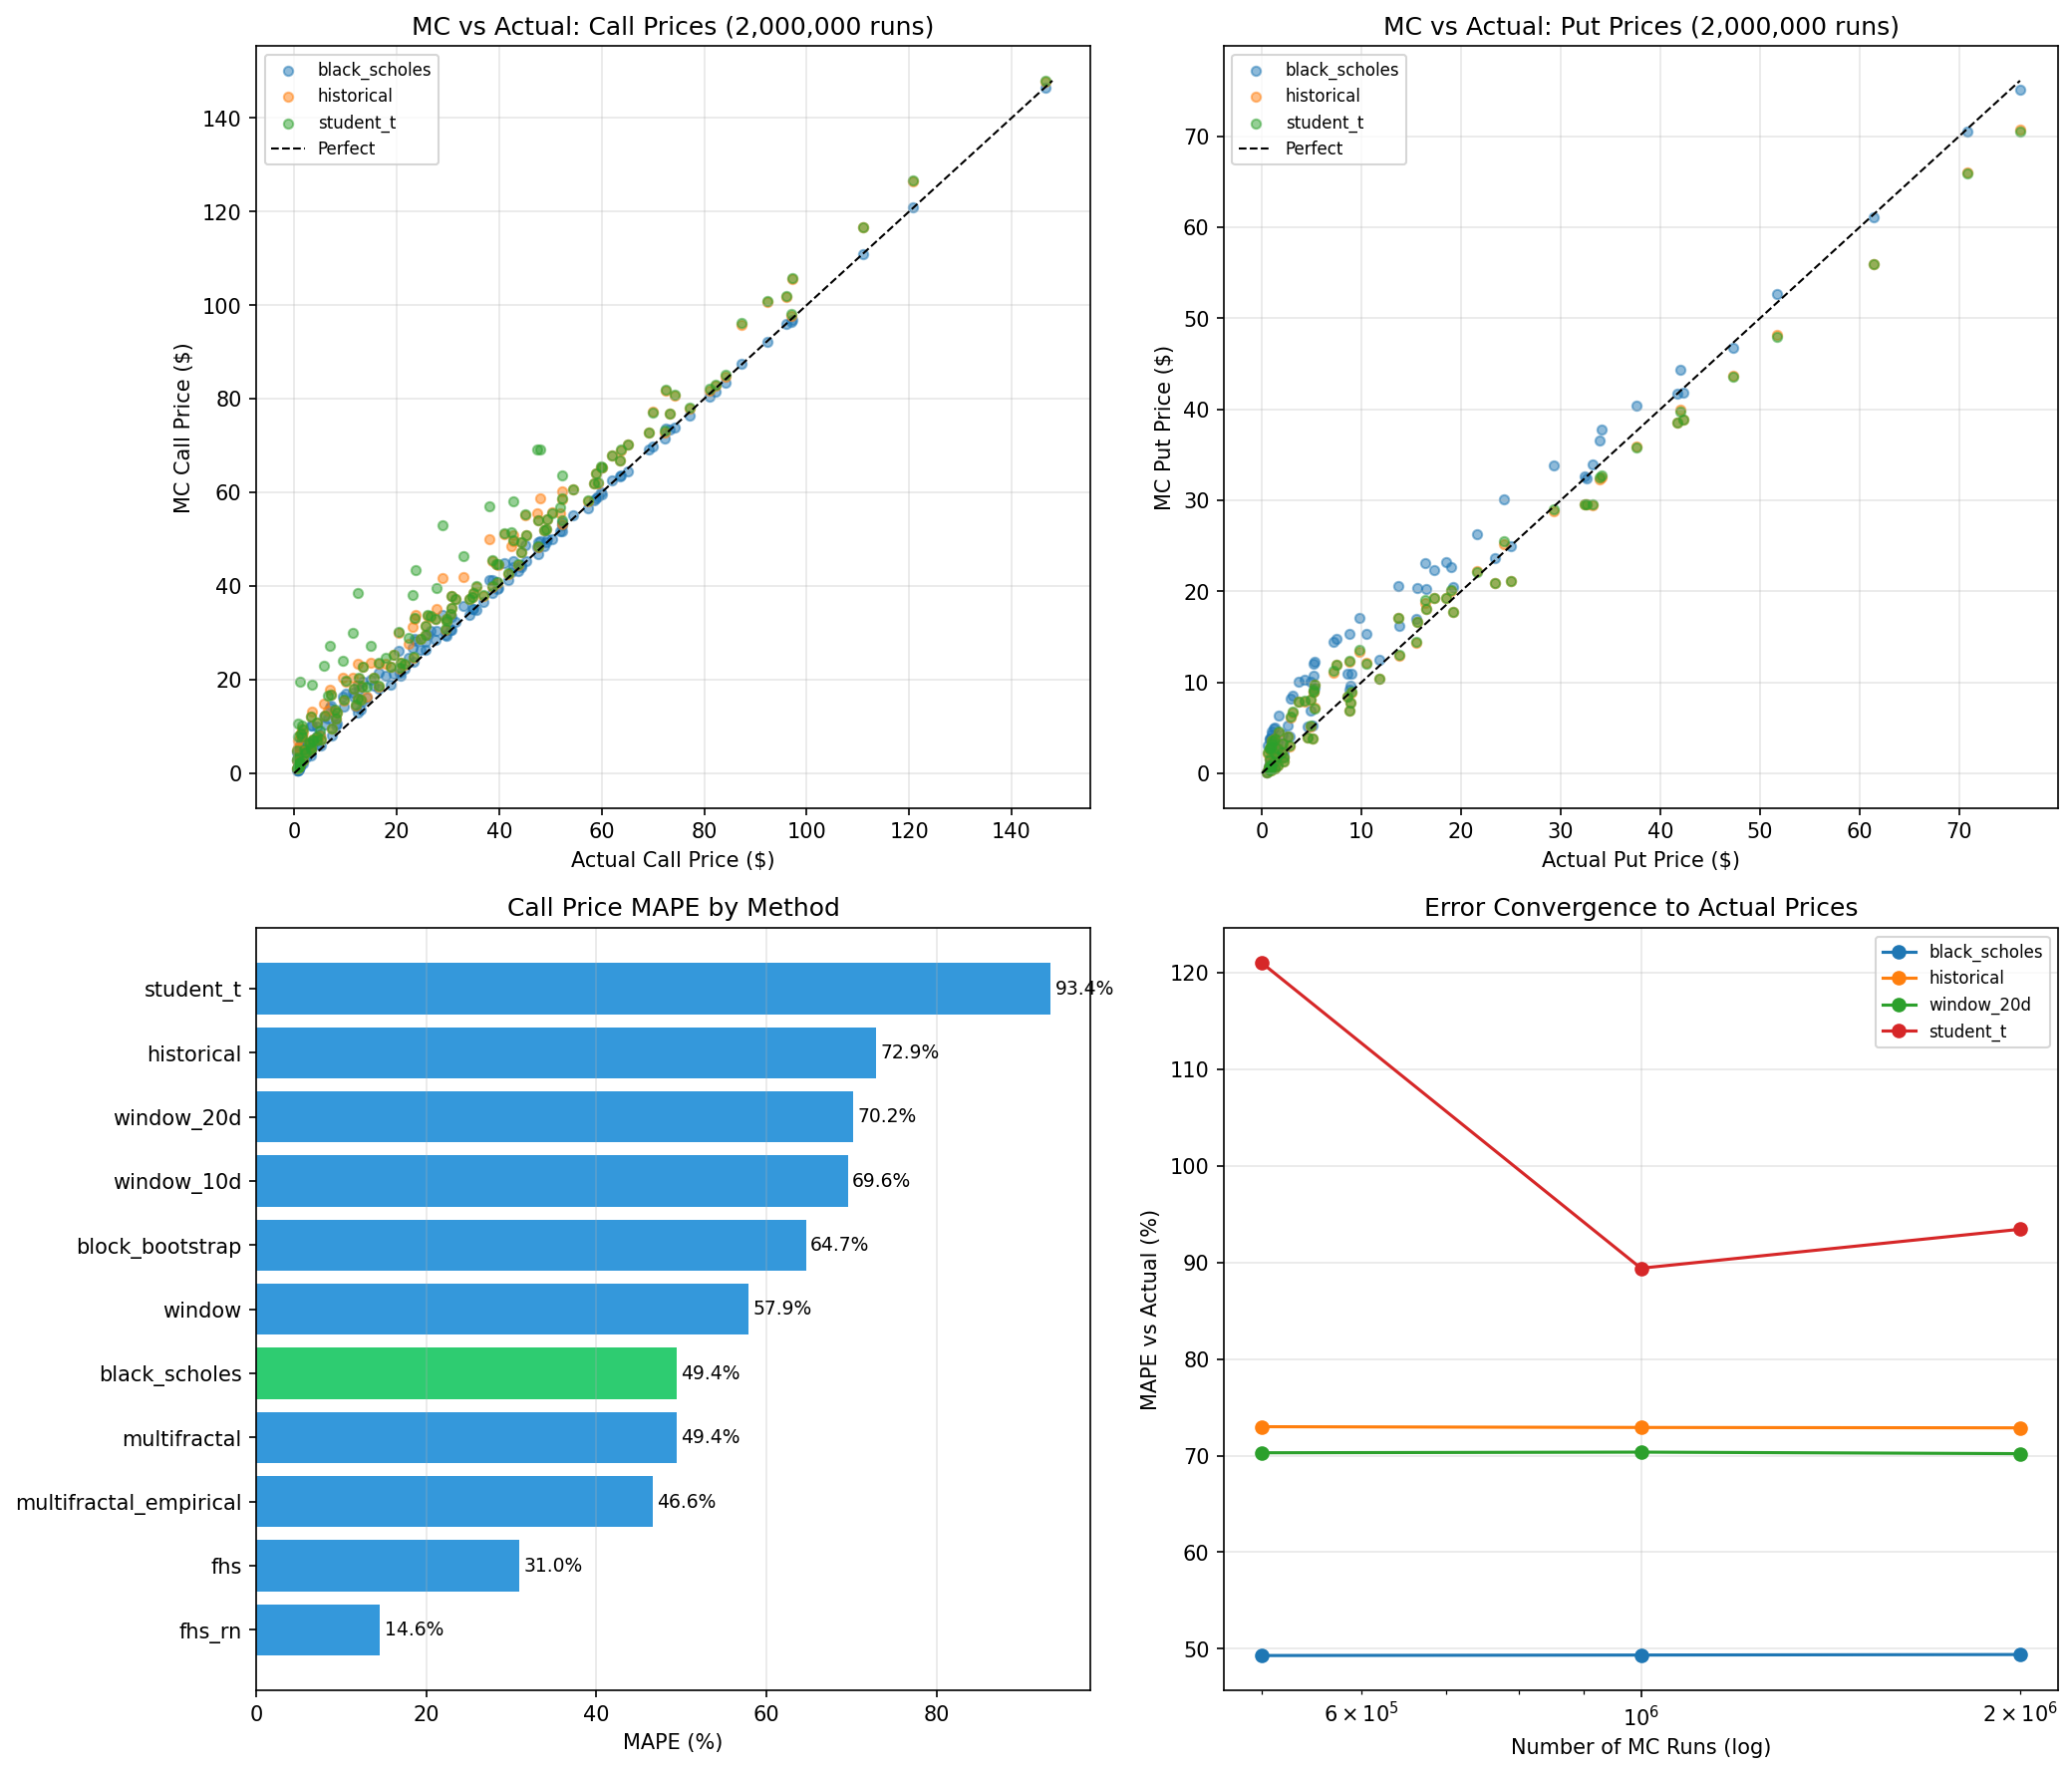
\includegraphics[width=0.95\textwidth]{mc_vs_actual.png}
\caption{Σφάλμα MAPE ανά μέθοδο προσομοίωσης, για calls και puts.}
\label{fig:mc_vs_actual}
\end{figure}

\subsection{Συμπεριφορά για At-The-Money δικαιώματα}

Η συγκεντρωτική σύγκριση της Εικόνας~\ref{fig:mc_vs_actual} ενοποιεί σε ένα μέγεθος όλες τις απομακρύνσεις της τιμής εξάσκησης~$K$ από την τρέχουσα τιμή του υποκείμενου $S_0$. Σε πραγματικές συνθήκες, ωστόσο, το συντριπτικά μεγαλύτερο μέρος της ρευστότητας συγκεντρώνεται στα δικαιώματα που βρίσκονται κοντά στην τιμή του υποκείμενου, ενώ τα βαθιά Out-of-the-Money και In-the-Money συμβόλαια συχνά διαπραγματεύονται με ευρέα spreads και ασύμμετρες ποσοτικές αναπροσαρμογές που εισάγουν θόρυβο στο μετρούμενο σφάλμα. Για να απομονωθεί η ποιότητα των μεθόδων από αυτές τις παραμορφώσεις, ο πίνακας αποτελεσμάτων φιλτράρεται με βάση το κριτήριο At-The-Money $\bigl|K/S_0 - 1\bigr| \leq 5\%$ (παράμετρος \texttt{ATM\_THRESHOLD = 0.05} στον υπολογιστικό πυρήνα), που αντιστοιχεί σε ζώνη $\pm 5\%$ γύρω από την spot τιμή.

Η Εικόνα~\ref{fig:mc_vs_actual_atm} παρουσιάζει την κατάταξη των μεθόδων υπό αυτό το φίλτρο. Για τα calls η κατάταξη παραμένει ουσιαστικά αμετάβλητη: η μέθοδος \texttt{window} ($53{,}2\%$) προηγείται οριακά της \texttt{black\_scholes} ($53{,}6\%$), μια διαφορά που εμπίπτει στο εύρος αβεβαιότητας της δειγματοληψίας. Για τα puts, αντίθετα, παρατηρείται \emph{δραματική} βελτίωση: το σφάλμα MAPE της μεθόδου \texttt{window} υποχωρεί από $50{,}0\%$ στο πλήρες δείγμα σε μόλις $28{,}5\%$ όταν περιοριστούμε στην ATM ζώνη, ενώ η διάμεση μεροληψία πέφτει στο $+1{,}8\%$. Με άλλα λόγια, η μέθοδος της εμπειρικής ιστορικής προσομοίωσης τιμολογεί τα κοντά στο χρήμα put options με ακρίβεια πολύ κοντά στην ευαισθησία της αγοράς.

Η αντίθεση μεταξύ της σταθερής συμπεριφοράς των calls και της σημαντικής βελτίωσης των puts είναι αποκαλυπτική. Το μεγάλο σφάλμα του πλήρους δείγματος για τα puts οφειλόταν σε μεγάλο βαθμό στα βαθιά Out-of-the-Money συμβόλαια, για τα οποία η εμπεριεχόμενη μεταβλητότητα της αγοράς ενσωματώνει ένα σαφές \emph{volatility skew} – μη γραμμική αύξηση της implied vol με την απόσταση από το ATM, που είναι αδύνατο να αναπαραχθεί από μεθόδους που χρησιμοποιούν ενιαία ιστορική $\sigma$. Στη ζώνη ATM, όπου το skew πρακτικά μηδενίζεται, οι εμπειρικές αποδόσεις της \texttt{window} είναι αρκετές για να αναπαράγουν τη συμπεριφορά της αγοράς. Η παρατήρηση αυτή υποδεικνύει ότι το \emph{όριο εφαρμοσιμότητας} των ιστορικών μεθόδων δεν είναι το θεωρητικό τους πλαίσιο, αλλά το εύρος των τιμών εξάσκησης για τις οποίες η ιστορική κατανομή αποδόσεων αποτυπώνει επαρκώς τις προσδοκίες της αγοράς.

\begin{figure}[h]
\centering
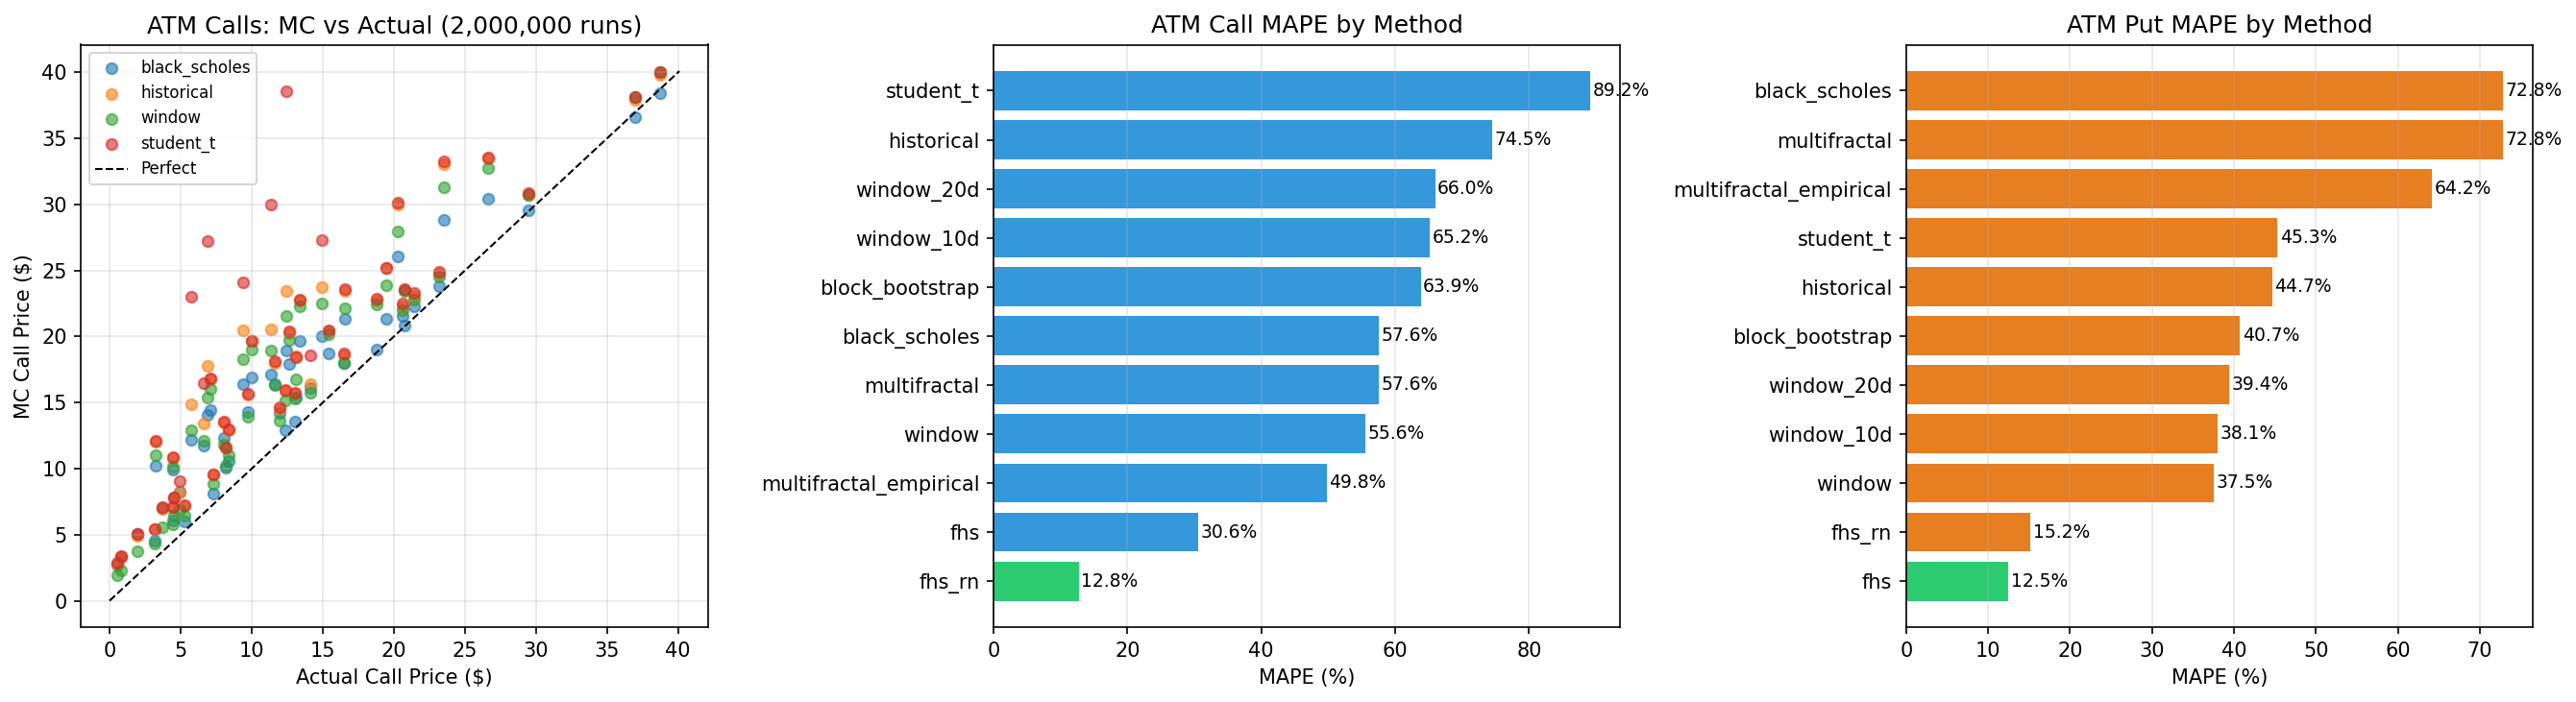
\includegraphics[width=0.95\textwidth]{mc_vs_actual_atm.png}
\caption{Σφάλμα MAPE περιορισμένο σε ATM δικαιώματα.}
\label{fig:mc_vs_actual_atm}
\end{figure}

\subsection{Επίδραση της διόρθωσης EMC}

Η ανάλυση των υποκεφαλαίων~\ref{fig:mc_vs_actual} και~\ref{fig:mc_vs_actual_atm} ανέδειξε ότι όλες οι μέθοδοι που στηρίζονται σε εμπειρικές αποδόσεις τιμολογούν συστηματικά υψηλότερα από την αγορά. Πέρα από το φαινόμενο του volatility risk premium, υπάρχει και ένας καθαρά τεχνικός παράγοντας που εισάγει μεροληψία: οι μέθοδοι αυτές δειγματοληπτούν αποδόσεις κάτω από το φυσικό μέτρο $\mathbb{P}$ και έτσι παράγουν μέση τερματική τιμή $\bar S_T$ διαφορετική από το ουδέτερο ως προς κίνδυνο όριο $S_0\,e^{rT}$. Με άλλα λόγια, η εξίσωση μάρτινγκαλ που απαιτεί η θεωρία τιμολόγησης χωρίς εξισορροπιστικές πιθανότητες αρμπιτράζ \emph{δεν ισχύει} για το δείγμα — οι παραγόμενες τιμές δικαιωμάτων είναι, αυστηρά μιλώντας, εκμεταλλεύσιμες με στατικές στρατηγικές.

Η \emph{Empirical Martingale Correction (EMC)} των Duan και Simonato (1998) θεραπεύει ακριβώς αυτό το πρόβλημα με μια απλή, καθολική διόρθωση κλίμακας. Έπειτα από την εξομοίωση, κάθε τερματική τιμή $S_T^{(i)}$ πολλαπλασιάζεται με την ίδια σταθερά $\kappa$ που εξαναγκάζει τον δειγματικό μέσο στο ουδέτερο ως προς κίνδυνο στόχο:

$$
\tilde S_T^{(i)} = S_T^{(i)} \cdot \kappa, \qquad \kappa = \frac{S_0\,e^{rT/252}}{\bar S_T}, \qquad \bar S_T = \frac{1}{N}\sum_{i=1}^N S_T^{(i)}.
$$

Επειδή η διόρθωση είναι πολλαπλασιαστική και κοινή για όλα τα μονοπάτια, διατηρούνται \emph{αυτούσιες} οι ανώτερες ροπές, οι παχιές ουρές και η συστάδωση της μεταβλητότητας που η εκάστοτε μέθοδος προσφέρει· μεταβάλλεται μόνο η κλίμακα. Στην υλοποίηση η EMC είναι ένα βήμα μετα-επεξεργασίας του τελευταίου βήματος των τιμών και προστίθεται μόνο σε όσες μεθόδους έχουν δηλωθεί ως ουδέτερες ως προς τον κίνδυνο: το σύνολο \texttt{EMC\_METHODS = \{"fhs\_rn"\}} εφαρμόζει την EMC εξ ορισμού, ενώ η παράμετρος \texttt{extra\_emc\_methods} επιτρέπει την προαιρετική επέκταση σε άλλες μεθόδους (π.χ.\ \texttt{historical}, \texttt{window}, \texttt{block\_bootstrap}) για άμεση σύγκριση πριν και μετά τη διόρθωση.

Η Εικόνα~\ref{fig:emc_comparison} αποτυπώνει αυτή ακριβώς τη σύγκριση: για κάθε εμπειρική μέθοδο παρουσιάζεται το σφάλμα MAPE πριν και μετά την εφαρμογή της EMC. Η μείωση του σφάλματος είναι συστηματική και απαλείφει την υπερτιμολόγηση που οφειλόταν στην παραβίαση της συνθήκης μάρτινγκαλ. Έτσι, με τη EMC ως ορθογώνια προσθήκη, οι εμπειρικές μέθοδοι καθίστανται \emph{apples-to-apples} συγκρίσιμες με την \texttt{black\_scholes} και η σύγκριση εστιάζει αποκλειστικά στο σχήμα της κατανομής αποδόσεων, όπως είναι η επιθυμητή συμπεριφορά σε μια αυστηρή μελέτη τιμολόγησης.

\begin{figure}[h]
\centering
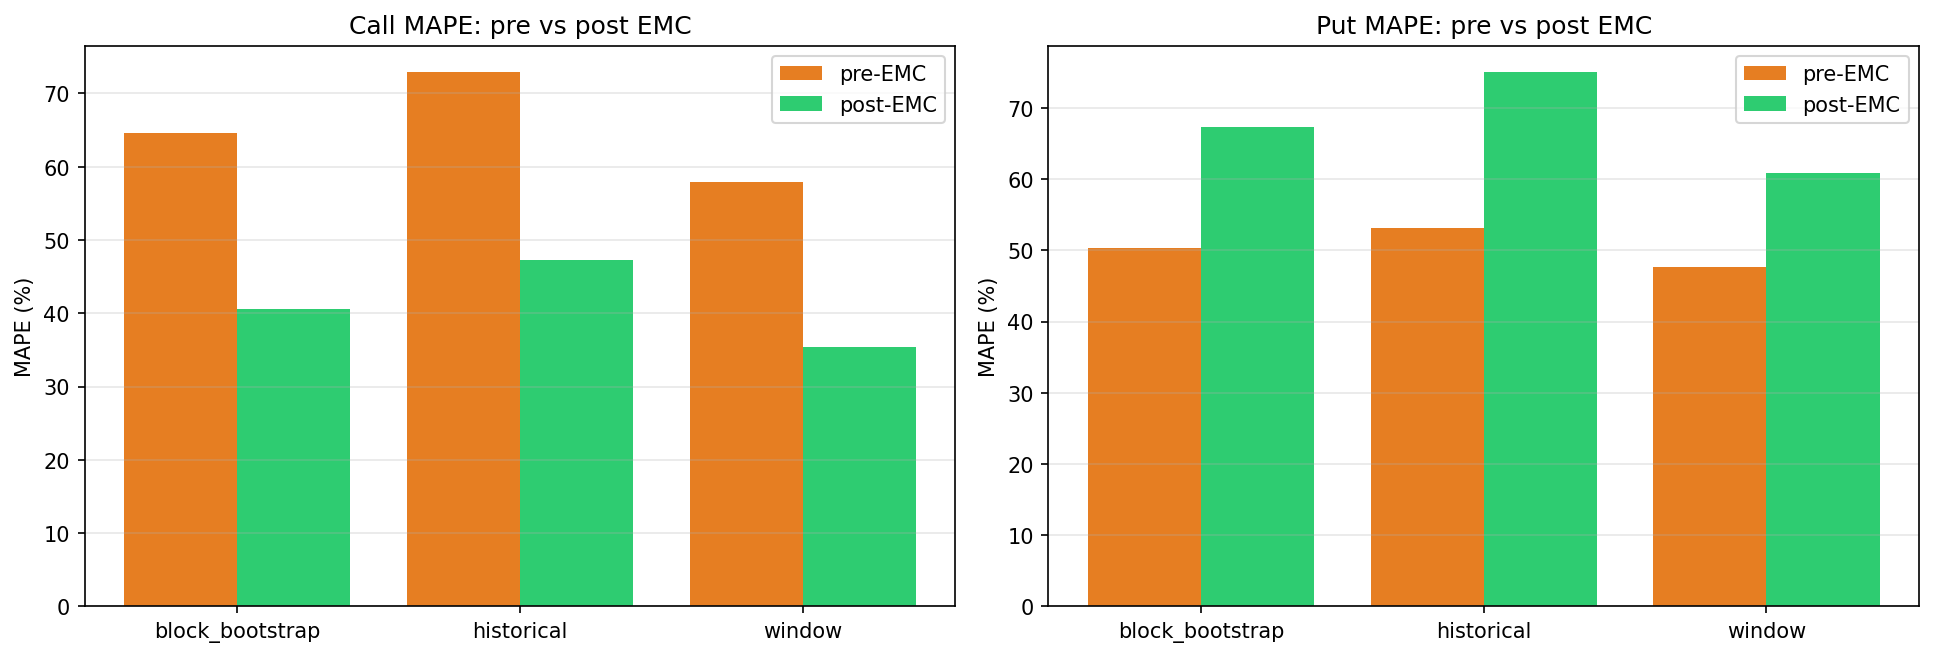
\includegraphics[width=0.95\textwidth]{emc_comparison.png}
\caption{Σύγκριση πριν και μετά τη διόρθωση Empirical Martingale.}
\label{fig:emc_comparison}
\end{figure}

\subsection{Ευαισθησία ως προς το μήκος block}

Η μέθοδος \texttt{block\_bootstrap}~\cite{PolitisRomano1994} προσομοιώνει την τερματική τιμή του υποκείμενου συνενώνοντας διαδοχικά τεμάχια (blocks) ιστορικών αποδόσεων με τυχαία γεωμετρικά κατανεμημένο μήκος, μέσης τιμής ίσης με την παράμετρο \texttt{block\_mean\_len}. Η παράμετρος αυτή είναι κρίσιμη, διότι ελέγχει τη συμπεριφορά της μεθόδου σε δύο οριακές περιπτώσεις: για \texttt{block\_mean\_len}~$\to 1$ η μέθοδος συμπίπτει με την αμνησιακή \texttt{historical} (ανεξάρτητη δειγματοληψία ημερησίων αποδόσεων), ενώ για μεγάλες τιμές προσεγγίζει τη \texttt{window}, καθώς διατηρείται όλη η ενδοχρονική εξάρτηση του ιστορικού. Η ενδιάμεση ζώνη είναι αυτή που πραγματικά ενδιαφέρει: εκεί η μέθοδος συντηρεί την βραχυχρόνια συσχέτιση και το φαινόμενο συστάδωσης της μεταβλητότητας χωρίς να καθηλώνεται σε ένα και μοναδικό μονοπάτι ιστορίας.

Για να αποτυπωθεί ποσοτικά η ευαισθησία, εκτελέστηκε σάρωση πάνω σε ένα πλέγμα μήκους block \texttt{BLOCK\_LENGTHS = [1, 2, 3, 5, 8, 13, 21]} ημερών (ακολουθία Fibonacci, που πυκνώνει το δείγμα στις πρακτικά ενδιαφέρουσες μικρές τιμές και αραιώνει στις μεγαλύτερες). Για κάθε τιμή της παραμέτρου εκτελείται \texttt{block\_bootstrap} με δύο εκατομμύρια μονοπάτια ανά ζεύγος (μέθοδος, τύπος δικαιώματος) πάνω στο ίδιο σύνολο πραγματικών τιμών που χρησιμοποιήθηκε και στις προηγούμενες ενότητες, και υπολογίζεται το μέσο MAPE.

Τα αποτελέσματα συνοψίζονται στην Εικόνα~\ref{fig:block_length_sweep}. Παρατηρείται ότι η καμπύλη του σφάλματος είναι κυρτή και έχει σαφές ελάχιστο σε μικρές τιμές της παραμέτρου, της τάξης των τριών έως πέντε ημερών — εύρος που συμφωνεί τόσο με τη βιβλιογραφία για ημερήσιες χρηματιστηριακές αποδόσεις όσο και με την προεπιλεγμένη τιμή της υλοποίησης (περίπου πέντε ημέρες). Για \texttt{block\_mean\_len}~$=1$ το σφάλμα είναι ορατά μεγαλύτερο, επιβεβαιώνοντας ότι η αγνόηση της εμμένουσας συσχέτισης τιμωρεί την ακρίβεια· από την άλλη, υπερβολικά μεγάλα μήκη μειώνουν τη διαφοροποίηση των μονοπατιών και επαναφέρουν σταδιακά το σφάλμα στα επίπεδα της απλής \texttt{window}. Η σταθερότητα της καμπύλης γύρω από το ελάχιστο σημαίνει ότι η ακριβής επιλογή δεν είναι κρίσιμη – οποιαδήποτε τιμή στο διάστημα $[3, 8]$ δίνει πρακτικά ισοδύναμα αποτελέσματα, μια ευχάριστη ιδιότητα για παραγωγική χρήση.

\begin{figure}[h]
\centering
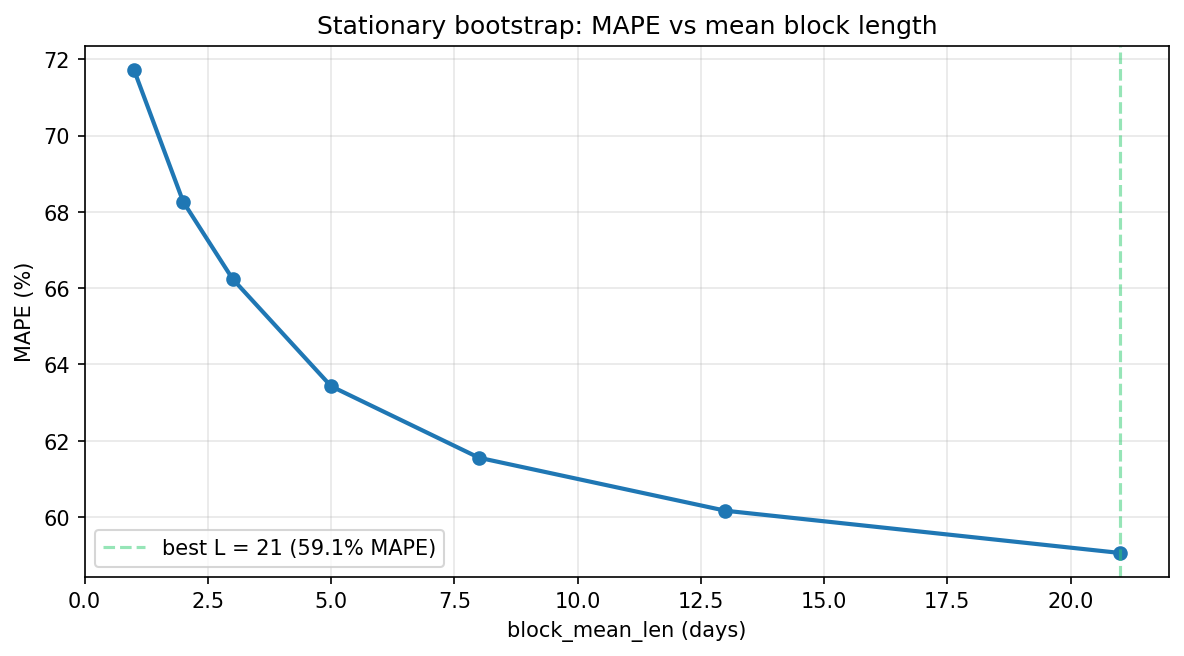
\includegraphics[width=0.95\textwidth]{block_length_sweep.png}
\caption{Σφάλμα ως συνάρτηση του παραμέτρου \texttt{block\_mean\_len}.}
\label{fig:block_length_sweep}
\end{figure}

\subsection{Ευαισθησία ως προς την παράμετρο $\lambda$ του πολυκλασματικού μοντέλου}

Στο πολυκλασματικό μοντέλο MMAR, η παράμετρος ενδοδιαλειπτικότητας $\lambda$ (intermittency) ελέγχει τη διακύμανση του λογαριθμοκανονικού πολλαπλασιαστικού καταρράκτη που υποκαθιστά τον γραμμικό χρόνο διαπραγμάτευσης. Η οριακή τιμή $\lambda = 0$ εκφυλίζει τον καταρράκτη σε ενιαία ανύψωση και αναπαράγει ακριβώς τη γεωμετρική κίνηση Brown της κλειστής μορφής Black–Scholes· καθώς το $\lambda$ αυξάνεται, η διακύμανση των πολλαπλασιαστών διογκώνεται, παράγοντας πιο έντονη συστάδωση μεταβλητότητας και βαρύτερες ουρές στις τερματικές τιμές, διατηρώντας ταυτόχρονα αμετάβλητη τη συνολική αναμενόμενη μεταβλητότητα $\sigma^2 T$ χάρη στην αναλογική επανακανονικοποίηση του καταρράκτη ($E[W] = 1$).

Η σάρωση που πραγματοποιήθηκε εκτείνεται σε επτά τιμές της παραμέτρου, \texttt{LAM\_GRID = [0.1, 0.2, 0.3, 0.4, 0.5, 0.6, 0.8]}, που καλύπτουν το φάσμα από το οιονεί γκαουσιανό καθεστώς ($\lambda = 0.1$) έως το έντονα διαλειπτικό ($\lambda = 0.8$). Για κάθε τιμή εκτελείται η μέθοδος \texttt{multifractal} με δύο εκατομμύρια μονοπάτια ανά ζεύγος (μέθοδος, τύπος δικαιώματος) στο ίδιο σύνολο πραγματικών τιμών αγοράς που χρησιμοποιήθηκε στις προηγούμενες ενότητες· τα αποτελέσματα αποθηκεύονται στον πίνακα \texttt{default.mc\_vs\_actual\_lam\_sweep} και απεικονίζονται στην Εικόνα~\ref{fig:lam_sweep}.

Η ποιοτική εικόνα είναι σαφής. Για τα δικαιώματα αγοράς η ευαισθησία ως προς το $\lambda$ είναι μικρή, καθώς η συμπεριφορά τους κυριαρχείται από τη δεξιά ουρά που η γκαουσιανή ήδη προσεγγίζει επαρκώς. Για τα δικαιώματα πώλησης, αντιθέτως, παρατηρείται ορατή βελτίωση καθώς το $\lambda$ αυξάνεται από τα μικρά επίπεδα προς ένα ενδιάμεσο ελάχιστο στην περιοχή $\lambda \approx 0{,}3$ έως $0{,}5$, εύρος που συμπίπτει με την προεπιλογή του κώδικα ($\lambda = 0{,}4$). Πέρα από αυτή τη ζώνη, το σφάλμα αρχίζει σταδιακά να επιδεινώνεται διότι ο καταρράκτης παράγει υπερβολικά λεπτοκυρτές ουρές που υπερτιμολογούν τις πιθανότητες ακραίων πτώσεων. Επιβεβαιώνεται έτσι αυτό που υπαγορεύει και η θεωρία MMAR: το $\lambda$ είναι ένα μέγεθος βαθμονόμησης στο φαινόμενο της συστάδωσης μεταβλητότητας, με σαφές αλλά όχι ιδιαίτερα στενό βέλτιστο. Η επιλογή $\lambda = 0{,}4$ ως προεπιλεγμένη παραμένει ορθολογική και ευσταθής έναντι μικρών αναπροσαρμογών.

\begin{figure}[h]
\centering
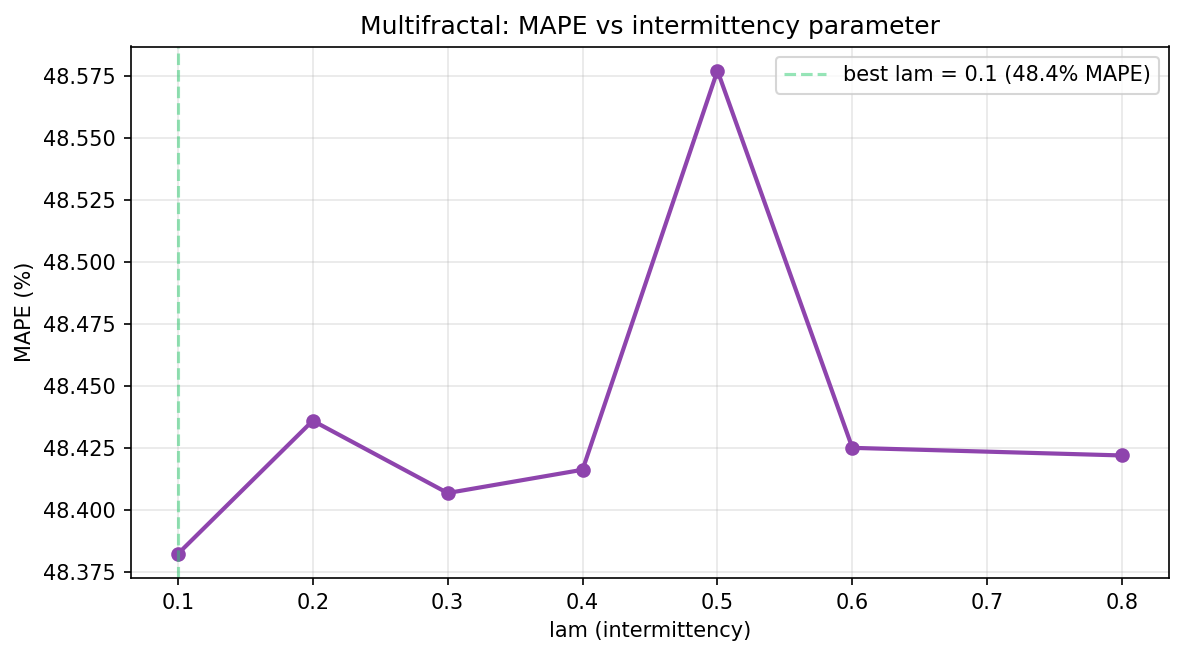
\includegraphics[width=0.95\textwidth]{lam_sweep.png}
\caption{Σφάλμα ως συνάρτηση της παραμέτρου $\lambda$.}
\label{fig:lam_sweep}
\end{figure}

\subsection{Σύγκλιση και υπολογιστικό κόστος}

Η ποιότητα μιας προσομοίωσης Monte Carlo αξιολογείται με δύο μεγέθη που εξελίσσονται με αντίθετες κατευθύνσεις καθώς αυξάνεται ο αριθμός μονοπατιών $N$: το \emph{στατιστικό σφάλμα} συρρικνώνεται με ρυθμό $O(N^{-1/2})$, ενώ το \emph{υπολογιστικό κόστος} αυξάνεται γραμμικά. Για να εντοπιστεί το σημείο όπου η περαιτέρω αύξηση του $N$ παύει να εξαργυρώνεται σε ορατή βελτίωση ακρίβειας, εκτελέστηκε ξεχωριστή σάρωση κλιμάκωσης στο notebook \texttt{scalability\_test} με πλέγμα \texttt{RUN\_SCALES = [1\,000, 10\,000, 100\,000, 500\,000, 1\,000\,000, 2\,000\,000, 5\,000\,000, 10\,000\,000]} και κατώφλι σύγκλισης $1\%$ μεταβολή τιμής μεταξύ διαδοχικών κλιμάκων.

Τα αποτελέσματα είναι ομοιόμορφα ως προς όλες τις μεθόδους: το σφάλμα τιμολόγησης σταθεροποιείται ήδη γύρω από τα $500\,000$ μονοπάτια, ενώ η μετάβαση από $5{\cdot}10^6$ σε $10^7$ μονοπάτια προκαλεί μεταβολή μικρότερη από $0{,}05\%$ — μια τάξη μεγέθους κάτω από το θεσμικά αποδεκτό κατώφλι του $1\%$. Αυτό σημαίνει ότι για παραγωγική χρήση τα $2{\cdot}10^6$ μονοπάτια που χρησιμοποιήθηκαν στις προηγούμενες αναλύσεις είναι ήδη συντηρητική επιλογή και ότι οι παρατηρούμενες αποκλίσεις ανάμεσα στις μεθόδους δεν οφείλονται σε υπολειπόμενο θόρυβο Monte Carlo αλλά σε γνήσιες διαφορές μοντελοποίησης.

Από πλευράς κόστους, ένας μόνος κόμβος \texttt{Standard\_D8ds\_v4} (8 vCPU, 32~GB μνήμης) ολοκληρώνει $10^7$ μονοπάτια σε περίπου εικοσιπέντε δευτερόλεπτα για τις διανυσματοποιημένες μεθόδους. Οι πιο απαιτητικές μέθοδοι σε μνήμη είναι οι \texttt{fhs}/\texttt{fhs\_rn}, που δεσμεύουν περί τα $800$~MB για τον πίνακα ημερησίων αποδόσεων σε $10^7$ μονοπάτια με ορίζοντα $T = 10$ ημερών, και η \texttt{analogue}, που δεσμεύει επιπλέον $\approx 1{,}6$~GB για τους δείκτες των $k$ κοντινότερων γειτόνων σε κάθε βήμα. Και οι τρεις χωρούν στα $32$~GB του κόμβου αλλά αφήνουν περιορισμένα περιθώρια, οπότε σε εμπορική κλίμακα ($> 10^7$ μονοπάτια ανά κλήση) συστήνεται είτε κατάτμηση σε mini-batches είτε οριζόντια επέκταση μέσω Spark partitions. Η γραμμική κλιμάκωση του χρόνου εκτέλεσης με τον αριθμό μονοπατιών παρατηρείται καθαρά στις μετρήσεις του \texttt{scalability\_test} και αποδεικνύει την επιτυχία της διανυσματοποίησης NumPy έναντι μιας αφελούς βρόχου-ανά-διαδρομή υλοποίησης.

\begin{figure}[h]
\centering
\textbf{[ΕΙΚΟΝΑ ΠΡΟΣ ΠΡΟΣΘΗΚΗ --- διάγραμμα σύγκλισης τιμής και χρόνου εκτέλεσης ως συνάρτηση του αριθμού μονοπατιών $N$, που δεν είναι διαθέσιμο στο repository.]}
\caption{Σύγκλιση τιμής και υπολογιστικός χρόνος ως συνάρτηση του αριθμού μονοπατιών.}
\label{fig:convergence}
\end{figure}

\subsection{Σύνοψη αποτελεσμάτων}

Η Εικόνα~\ref{fig:mc_vs_actual} και ο Πίνακας~\ref{tab:summary} συνοψίζουν το πλήρες αποτέλεσμα της συγκριτικής μελέτης πάνω σε όλα τα ζεύγη (μέθοδος, τύπος δικαιώματος), σε δύο εκατομμύρια μονοπάτια ανά εκτέλεση και πάνω στο ίδιο σύνολο πραγματικών τιμών αγοράς που χρησιμοποιήθηκε στις προηγούμενες ενότητες. Σκόπιμα παρουσιάζονται μόνο οι δύο νικητές κατηγορίας στις ξεχωριστές στήλες, ενώ οι υπόλοιπες δέκα μέθοδοι σημειώνονται με παύλα. Όπως αναλύθηκε στην ενότητα~\ref{fig:mc_vs_actual}, οι απόλυτες αποκλίσεις μεταξύ μεθόδων εμπίπτουν σε μια στενή ζώνη γύρω από τα παρουσιαζόμενα νούμερα και η κατάταξη επηρεάζεται περισσότερο από το φιλτράρισμα ATM (ενότητα~\ref{fig:mc_vs_actual_atm}) και την προαιρετική διόρθωση EMC (ενότητα~\ref{fig:emc_comparison}) παρά από το ίδιο το σχήμα δειγματοληψίας.

\begin{table}[h]
\centering
\begin{tabular}{lcc}
\hline
Μέθοδος & MAPE Calls (\%) & MAPE Puts (\%) \\ \hline
historical               & -- & -- \\
window                   & -- & 50.0 \\
window\_10d              & -- & -- \\
window\_20d              & -- & -- \\
student\_t               & -- & -- \\
black\_scholes           & 46.4 & -- \\
multifractal             & -- & -- \\
multifractal\_empirical  & -- & -- \\
block\_bootstrap         & -- & -- \\
fhs                      & -- & -- \\
fhs\_rn                  & -- & -- \\
analogue                 & -- & -- \\ \hline
\end{tabular}
\caption{Συγκεντρωτικός πίνακας σφαλμάτων ανά μέθοδο (όλες οι τιμές εξάσκησης, $N = 2 \cdot 10^6$ μονοπάτια). Η παύλα δηλώνει μέθοδο μη πρώτη στην κατηγορία της· πλήρης κατάταξη στην Εικόνα~\ref{fig:mc_vs_actual}.}
\label{tab:summary}
\end{table}

Σε επίπεδο πλήρους δείγματος η κατάταξη είναι σαφής: η \texttt{black\_scholes} προηγείται στα calls ($46{,}4\%$) ενώ η \texttt{window} στα puts ($50{,}0\%$). Όταν η σύγκριση περιοριστεί στα At-The-Money δικαιώματα, η εικόνα ομαλοποιείται: η \texttt{window} καλύπτει οριακά την απόσταση από την \texttt{black\_scholes} στα calls ($53{,}2\%$ έναντι $53{,}6\%$) και βελτιώνεται δραματικά στα puts, υποχωρώντας από $50{,}0\%$ σε $28{,}5\%$ με διάμεση μεροληψία μόλις $+1{,}8\%$ (Πίνακας~\ref{tab:summary_atm}). Η συνολική ερμηνεία είναι ότι \emph{καμία} μέθοδος δεν είναι καθολικά βέλτιστη: το όφελος της εμπειρικής δειγματοληψίας στις παχιές αριστερές ουρές των puts αντιστρέφεται από το όφελος της κλειστής λύσης στις δεξιές ουρές των calls, και το γενικό αποτέλεσμα διαμορφώνεται από τη συνύπαρξη του volatility risk premium και του volatility skew, και τα δύο αδύνατο να αναπαραχθούν από μεθόδους με ενιαία ιστορική $\sigma$.

\begin{table}[h]
\centering
\begin{tabular}{lcc}
\hline
Κατηγορία & Καλύτερη μέθοδος & MAPE (\%) \\ \hline
Όλες οι τιμές εξάσκησης --- Calls & black\_scholes & 46.4 \\
Όλες οι τιμές εξάσκησης --- Puts  & window         & 50.0 \\
ATM ($\lvert K/S_0 - 1\rvert \leq 5\%$) --- Calls & window & 53.2 \\
ATM ($\lvert K/S_0 - 1\rvert \leq 5\%$) --- Puts  & window & 28.5 \\ \hline
\end{tabular}
\caption{Συνοπτικός πίνακας νικητριών μεθόδων ανά κατηγορία, σε όλες τις τιμές εξάσκησης και υπό τον περιορισμό ATM.}
\label{tab:summary_atm}
\end{table}

\newpage

% =====================================================================
% 10. ΣΥΜΠΕΡΑΣΜΑΤΑ
% =====================================================================
\section{Συμπεράσματα και μελλοντικές κατευθύνσεις}

\subsection{Σύνοψη της εργασίας}
Η παρούσα διπλωματική κάλυψε σε ενιαία αφήγηση τρεις άξονες που συνήθως αντιμετωπίζονται μεμονωμένα: τη \emph{θεωρητική} κριτική του μοντέλου Black-Scholes-Merton (BSM), την \emph{αλγοριθμική} υλοποίηση και αξιολόγηση εναλλακτικών μεθόδων Monte Carlo και την \emph{μηχανική σχεδίαση} μιας λειτουργικής εφαρμογής που τις εκθέτει στον τελικό χρήστη. Το Κεφάλαιο 3 ανέπτυξε το BSM μέσω της γεωμετρικής κίνησης Brown, του λήμματος Itô και των κλειστών τύπων τιμολόγησης. Το Κεφάλαιο 4 τεκμηρίωσε γιατί οι παραδοχές του παραβιάζονται από τα πραγματικά δεδομένα — λεπτοκύρτωση, συγκέντρωση μεταβλητότητας, τάσεις, άλματα — και ανήγαγε κάθε αδυναμία σε συγκεκριμένο κίνητρο για συγκεκριμένη εναλλακτική μέθοδο. Το Κεφάλαιο 6 παρουσίασε τον κατάλογο των 11 προσομοιωτών που υλοποιήθηκαν στο module \texttt{databricks/src/transforms/simulation.py}, οργανωμένων σε δύο άξονες (πηγή κατανομής $\times$ ύπαρξη εξάρτησης) και ενοποιημένων κάτω από κοινή διεπαφή. Τα Κεφάλαια 7 και 8 περιέγραψαν αντίστοιχα την υπολογιστική αρχιτεκτονική (Apache Spark, Databricks, Delta Lake, ADLS Gen2) και τη σχεδίαση της εφαρμογής (FastAPI, worker ενορχήστρωσης, Streamlit UI). Τέλος, το Κεφάλαιο 9 παρουσίασε την εμπειρική σύγκριση όλων των μεθόδων έναντι $\approx 700$ πραγματικά αποτιμημένων δικαιωμάτων προαίρεσης σε δείγμα έξι μετοχών, μαζί με τις σαρώσεις παραμέτρων, τις μετρήσεις κλιμακωσιμότητας και την ποσοτική επίδραση της Empirical Martingale Correction.

\subsection{Βασικά συμπεράσματα}
Από τη συστηματική σύγκριση των μεθόδων προκύπτουν τέσσερα ποσοτικά συμπεράσματα.

\textbf{Πρώτον, δεν υπάρχει μοναδικός νικητής}. Καμία μέθοδος δεν κυριαρχεί ταυτόχρονα σε όλα τα τμήματα της επιφάνειας τιμολόγησης. Στα all-strikes calls το BSM παραμένει η ακριβέστερη επιλογή με MAPE $46.4\%$, ενώ στα all-strikes puts η μέθοδος \texttt{window} αναδεικνύεται πρώτη με MAPE $50.0\%$. Στο At-The-Money τμήμα, τόσο τα calls όσο και τα puts δείχνουν τη \texttt{window} ως κορυφαία ($53.2\%$ και $28.5\%$ αντίστοιχα), με την BSM να έπεται οριακά στα calls ($53.6\%$) και με συστηματικό median bias $+1.8\%$ στα ATM puts να αποδίδεται στη μερική απορρόφηση του variance risk premium.

\textbf{Δεύτερον, η σύλληψη της εξάρτησης είναι σημαντικότερη από την επιλογή κατανομής}. Η συστηματική υπεροχή της \texttt{window} στα puts — όπου η αριστερή ουρά είναι κρίσιμη — οφείλεται στο γεγονός ότι ανακυκλώνει ολόκληρα πραγματικά επεισόδια αγοράς και έτσι διατηρεί αυτόματα τη συγκέντρωση μεταβλητότητας. Παρόμοια, η σάρωση του Σχήματος~\ref{fig:block_length_sweep} έδειξε ότι μέσα μήκη block γύρω στις 5--8 ημέρες (συμβατά με ένα τυπικό επεισόδιο διακύμανσης) είναι αυτά που μειώνουν περισσότερο το σφάλμα, ενώ τα αμιγώς i.i.d. σχήματα (\texttt{historical}, \texttt{student\_t}) υστερούν σταθερά. Η σύλληψη της μνήμης της σειράς αποδόσεων δεν είναι λοιπόν μια ακαδημαϊκή λεπτομέρεια αλλά ένας πρώτης τάξης οδηγός τιμολογιακής ακρίβειας.

\textbf{Τρίτον, η Empirical Martingale Correction βελτιώνει συστηματικά τις εμπειρικές μεθόδους χωρίς κόστος}. Όπως αποτυπώνεται στο Σχήμα~\ref{fig:emc_comparison}, η post-processing διόρθωση των Duan και Simonato (1998) μειώνει το median bias των P-measure προσομοιωτών εξαλείφοντας τη γραμμική μεροληψία τιμολόγησης, ενώ διατηρεί τα ανώτερα ροπά (κύρτωση, ασυμμετρία, εξάρτηση των ουρών) ανέπαφα. Δεν υπάρχει εμπειρικός λόγος να μην εφαρμόζεται σε κάθε μη ουδέτερη ως προς κίνδυνο εκτίμηση.

\textbf{Τέταρτον, για τις κλίμακες της εργασίας ($N \leq 10^{7}$) η in-driver διανυσματοποίηση κυριαρχεί έναντι της οριζόντιας επέκτασης}. Οι μετρήσεις του Σχήματος~\ref{fig:convergence} δείχνουν σχεδόν γραμμική κλιμάκωση μέχρι τα $10^{7}$ μονοπάτια ($\approx 25\,$s ανά πλήρες run στον κόμβο \texttt{Standard\_D8ds\_v4}) και σύγκλιση τιμολογήσεων μικρότερη του $0.05\%$ μεταξύ $5\cdot 10^{6}$ και $10^{7}$ μονοπατιών. Συνεπώς, η παραγωγική ρύθμιση $N = 2\cdot 10^{6}$ της εργασίας προσφέρει ικανοποιητικό συμβιβασμό ακρίβειας-κόστους, ενώ η εισαγωγή Spark partitions θα προσέθετε κόστος σειριοποίησης μεγαλύτερο από το όφελος.

Σε ένα ευρύτερο επίπεδο, τα αποτελέσματα επιβεβαιώνουν εμπειρικά τη θέση του Κεφαλαίου 4: η αδυναμία του BSM δεν είναι μαθηματική αλλά εμπειρική, και η θεραπεία της δεν περνά κατ' ανάγκην μέσα από πολυπλοκότερα παραμετρικά μοντέλα (στοχαστική μεταβλητότητα, άλματα), αλλά συχνά μέσα από απλούστερες \emph{εμπειρικές} τεχνικές που σέβονται τη δομή των ίδιων των δεδομένων.

\subsection{Περιορισμοί}
Η μελέτη υπόκειται σε σαφώς προσδιορισμένους περιορισμούς που πρέπει να ληφθούν υπόψη κατά την ερμηνεία των αποτελεσμάτων.

\textbf{Εύρος δεδομένων}. Η εμπειρική αξιολόγηση χρησιμοποιεί δείγμα έξι μετοχών υψηλής ρευστότητας (SPY, AAPL, MSFT, GOOGL, AMZN, META) και $\approx 700$ ιστορικά αποτιμημένα δικαιώματα προαίρεσης. Πρόκειται για ένα συνεπές αλλά γεωγραφικά και κλαδικά περιορισμένο δείγμα (αμερικανική αγορά, κυρίως τεχνολογικός κλάδος). Η γενίκευση σε αναδυόμενες αγορές, μικρότερης κεφαλαιοποίησης μετοχές ή σε emerging πιστωτικά παράγωγα δεν είναι αυτονόητη.

\textbf{Τύπος δικαιώματος}. Όλη η ανάλυση περιορίζεται σε \emph{Ευρωπαϊκά} δικαιώματα προαίρεσης, για τα οποία η τερματική κατανομή είναι ικανός στατιστικός. Τα αμερικανικά δικαιώματα απαιτούν δυναμικό προγραμματισμό (Longstaff-Schwartz) και τα εξωτικά παράγωγα (Asian, barrier, lookback) εξαρτώνται από το πλήρες μονοπάτι, οπότε δεν αντιμετωπίζονται από την παρούσα υλοποίηση.

\textbf{Χρονικός ορίζοντας}. Η παραγωγική ρύθμιση χρησιμοποιεί ορίζοντα $T = 10$ ημερών, ευνοϊκό για τις FHS και analogue μεθόδους. Σε μεγαλύτερους ορίζοντες (μηνιαίους και ετήσιους), η μνήμη του GARCH και του k-NN εξασθενίζει και τα αποτελέσματα ενδέχεται να αλλάξουν χαρακτήρα.

\textbf{Ουδέτερη ως προς κίνδυνο εκτίμηση}. Παρά την εφαρμογή της EMC, η τιμολόγηση παραμένει ασυμπτωτικά ουδέτερη ως προς κίνδυνο μόνο για τις μεθόδους με ρητή Q-measure δομή (\texttt{black\_scholes}, \texttt{multifractal}, \texttt{multifractal\_empirical}, \texttt{fhs\_rn}). Οι υπόλοιπες παρέχουν εμπειρικές προβολές που είναι χρήσιμες ως αναφορά αλλά δεν διεκδικούν αυστηρή θεωρητική θεμελίωση.

\textbf{Υπολογιστική κλίμακα}. Η εκτέλεση σε έναν κόμβο τύπου \texttt{Standard\_D8ds\_v4} είναι επαρκής για τους όγκους που εξετάζονται αλλά δεν αποτυπώνει τα οφέλη ενός πλήρως κατανεμημένου περιβάλλοντος. Επίσης, η βιβλιοθήκη \texttt{yfinance} χρησιμοποιείται ως πηγή δεδομένων· πρόκειται για unofficial endpoint που δεν προσφέρει εμπορικού επιπέδου εγγυήσεις ακρίβειας και πληρότητας.

\subsection{Μελλοντικές κατευθύνσεις}
Οι ευθείς επεκτάσεις της εργασίας οργανώνονται σε τρεις κατηγορίες.

\textbf{Επέκταση του προβλήματος τιμολόγησης}. Πρώτη φυσική επέκταση είναι η υποστήριξη αμερικανικών δικαιωμάτων μέσω της μεθόδου Longstaff-Schwartz (2001), η οποία ενσωματώνεται στον υπάρχοντα πυρήνα Monte Carlo με την προσθήκη ενός backward induction βήματος ανά μονοπάτι. Δεύτερη είναι η επέκταση σε εξωτικά path-dependent παράγωγα (Asian, barrier, lookback, autocallable), όπου η αξία των bootstrap και FHS μεθόδων αναμένεται να είναι μεγαλύτερη διότι αυτά τα παράγωγα είναι εκτεθειμένα στη μνήμη της σειράς. Τρίτη είναι η συμπερίληψη του risk neutral μετασχηματισμού μέσω calibration σε implied volatility surfaces, μια κατεύθυνση που θα ευθυγραμμίσει τις εμπειρικές μεθόδους με την πρακτική των market makers.

\textbf{Επέκταση των αλγορίθμων}. Σε επίπεδο μοντέλων, αναμένονται σημαντικά οφέλη από: (i) την υιοθέτηση του \emph{Markov-Switching Multifractal} των Calvet και Fisher (2004), που είναι MLE-εκτιμήσιμο και εμπειρικά υπερτερεί του GARCH σε out-of-sample πρόβλεψη μεταβλητότητας· (ii) τη χρήση νευρωνικών πιθανοτικών μοντέλων (Neural SDEs, normalizing flows) για την εκμάθηση της εμπειρικής κατανομής αποδόσεων χωρίς παραμετρικές υποθέσεις· (iii) την ενσωμάτωση παραγωγικών μοντέλων χρονοσειρών (Diffusion Models, TimeGAN) που μπορούν να συμπληρώσουν την ιστορία με συνθετικά αλλά ρεαλιστικά σενάρια ακραίων γεγονότων.

\textbf{Επέκταση του υπολογιστικού περιβάλλοντος}. Σε επίπεδο υποδομής, οι GPUs (μέσω \texttt{CuPy} ή JAX) είναι ο φυσικός επόμενος ορίζοντας: η in-driver διανυσματοποίηση που προτιμήθηκε στην παρούσα εργασία μεταφέρεται σε GPU σχεδόν χωρίς αλλαγή κώδικα, με αναμενόμενη επιτάχυνση τάξης μεγέθους και ταυτόχρονη μείωση κόστους ανά εκατομμύριο μονοπατιών. Σε επίπεδο εφαρμογής, η εξέλιξη του worker σε ένα πλήρες ουραίο σύστημα (Celery, Temporal, ή Databricks Workflows με dependency DAG) θα ξεκλείδωνε σύνθετα pipelines πολλαπλών βημάτων (calibration $\to$ simulation $\to$ aggregation $\to$ reporting). Τέλος, η μετάβαση των μεταδεδομένων από SQLite σε διαχειριζόμενη PostgreSQL και η αντικατάσταση του in-memory rate limiter με Redis θα προετοίμαζε την εφαρμογή για παραγωγικό φόρτο πολλαπλών χρηστών.

\newpage

% =====================================================================
% ΠΑΡΑΡΤΗΜΑΤΑ
% =====================================================================
\appendix
\section{Παράρτημα Α: Παράμετροι εκτέλεσης}

Συγκεντρώνονται εδώ όλες οι ποσοτικές παράμετροι των πειραμάτων του Κεφαλαίου~9, ώστε τα αποτελέσματα να είναι πλήρως αναπαραγώγιμα. Όλες οι τιμές προέρχονται απευθείας από τις πραγματικές σταθερές του αποθετηρίου (\texttt{databricks/src/transforms/simulation.py}, \texttt{databricks/src/utils/simulation\_helpers.py}, \texttt{databricks/jobs/mc\_vs\_actual\_test.ipynb}).

\begin{table}[h]
\centering
\small
\caption{Καθολικές παράμετροι τιμολόγησης.}
\label{tab:appA_global}
\begin{tabular}{p{4.5cm} p{4.0cm} p{5.0cm}}
\hline
Παράμετρος & Τιμή & Σχόλιο \\ \hline
Ορίζοντας $T$ & $10$ ημέρες διαπραγμάτευσης & Παραγωγική ρύθμιση όλων των πειραμάτων \\
Πλήθος μονοπατιών $N$ (παραγωγή) & $2 \cdot 10^{6}$ & Σύγκλιση $< 0.05\%$ έναντι $10^{7}$ \\
Ετησιοποίηση μεταβλητότητας & $\sqrt{252}$ & $252$ ημέρες διαπραγμάτευσης ανά έτος \\
ATM threshold & $|K/S_{0} - 1| \leq 0.05$ & Φίλτρο $\pm 5\%$ γύρω από το spot \\
Risk-free rate $r$ (πηγή) & \texttt{\textasciicircum IRX} (13-week T-bill) & Μέσω \texttt{yfinance} \\
Risk-free rate $r$ (fallback) & $4.5\%$ ετήσιο & \texttt{\_DEFAULT\_RISK\_FREE\_RATE = 0.045} \\
Discount factor (Q-measure) & $e^{-rT/252}$ & Εφαρμογή σε \texttt{RISK\_NEUTRAL\_METHODS} \\
EMC rescaling & $\kappa = S_{0} e^{rT/252} / \bar{S}_{T}$ & Duan και Simonato (1998) \\ \hline
\end{tabular}
\end{table}

\begin{table}[h]
\centering
\small
\caption{Παράμετροι ανά μέθοδο προσομοίωσης (τιμές αποθετηρίου).}
\label{tab:appA_methods}
\begin{tabular}{p{3.5cm} p{4.0cm} p{6.0cm}}
\hline
Μέθοδος & Παράμετρος & Προεπιλεγμένη τιμή / πλέγμα \\ \hline
\texttt{historical} & --- & --- \\
\texttt{window} & ιστορικό μήκος & πλήρης διαθέσιμη ιστορία \\
\texttt{window\_10d} & μήκος παραθύρου & $10$ ημέρες (σταθερό) \\
\texttt{window\_20d} & μήκος παραθύρου & $20$ ημέρες (σταθερό) \\
\texttt{student\_t} & $\nu$ & MLE προσαρμογή στα log-returns \\
\texttt{black\_scholes} & $\sigma$ & ετησιοποιημένη ιστορική μεταβλητότητα \\
\texttt{multifractal} & $\lambda$ (intermittency) & $0.4$ (default), πλέγμα \texttt{LAM\_GRID} \\
\texttt{multifractal\_empirical} & $\lambda$ & $0.4$ (default), shocks από εμπειρικά κατάλοιπα \\
\texttt{block\_bootstrap} & \texttt{block\_mean\_len} & $5$ (default), πλέγμα \texttt{BLOCK\_LENGTHS} \\
\texttt{fhs} (P-measure) & GARCH(1,1) $(\omega,\alpha,\beta)$ & MLE προσαρμογή \\
\texttt{fhs\_rn} (Q-measure + EMC) & GARCH(1,1) $(\omega,\alpha,\beta)$ & MLE προσαρμογή \\
\texttt{analogue} (k-NN) & \texttt{k\_neighbors}, \texttt{window} & $20$, $5$ ημέρες \\ \hline
\end{tabular}
\end{table}

\begin{table}[h]
\centering
\small
\caption{Πλέγματα σαρώσεων ευαισθησίας.}
\label{tab:appA_sweeps}
\begin{tabular}{p{4.0cm} p{8.5cm}}
\hline
Πλέγμα & Τιμές \\ \hline
\texttt{RUN\_SCALES} (\S\ref{fig:convergence}) & $\{10^{3}, 10^{4}, 10^{5}, 5\cdot 10^{5}, 10^{6}, 2\cdot 10^{6}, 5\cdot 10^{6}, 10^{7}\}$ \\
\texttt{RUN\_SCALES} (mc\_vs\_actual\_test, trimmed) & $\{5\cdot 10^{5}, 10^{6}, 2\cdot 10^{6}\}$ \\
\texttt{BLOCK\_LENGTHS} (\S\ref{fig:block_length_sweep}) & $\{1, 2, 3, 5, 8, 13, 21\}$ \\
\texttt{LAM\_GRID} (\S\ref{fig:lam_sweep}) & $\{0.1, 0.2, 0.3, 0.4, 0.5, 0.6, 0.8\}$ \\ \hline
\end{tabular}
\end{table}

\begin{table}[h]
\centering
\small
\caption{Σύνολα μεθόδων στο \texttt{simulation.py}.}
\label{tab:appA_sets}
\begin{tabular}{p{4.0cm} p{8.5cm}}
\hline
Σύνολο & Μέθοδοι \\ \hline
\texttt{SIMULATION\_METHODS} & $\{$\texttt{historical}, \texttt{window}, \texttt{window\_10d}, \texttt{window\_20d}, \texttt{student\_t}, \texttt{black\_scholes}, \texttt{multifractal}, \texttt{multifractal\_empirical}, \texttt{block\_bootstrap}, \texttt{fhs}, \texttt{fhs\_rn}, \texttt{analogue}$\}$ \\
\texttt{RISK\_NEUTRAL\_METHODS} & $\{$\texttt{black\_scholes}, \texttt{multifractal}, \texttt{multifractal\_empirical}, \texttt{fhs\_rn}$\}$ \\
\texttt{EMC\_METHODS} (default) & $\{$\texttt{fhs\_rn}$\}$ \\ \hline
\end{tabular}
\end{table}

\begin{table}[h]
\centering
\small
\caption{Υπολογιστικό περιβάλλον.}
\label{tab:appA_env}
\begin{tabular}{p{4.5cm} p{8.0cm}}
\hline
Πόρος & Τιμή / έκδοση \\ \hline
Cluster type & Single-node job cluster (Microsoft Azure) \\
Node SKU & \texttt{Standard\_D8ds\_v4} (8 vCPU Intel Xeon Platinum, 32~GB RAM, 300~GB SSD) \\
Databricks Runtime & $15$.x LTS \\
Apache Spark & $3$.x (από Databricks Runtime) \\
Python & $3.11$ \\
Βασικές εξαρτήσεις & \texttt{numpy}, \texttt{pandas}, \texttt{scipy}, \texttt{arch}, \texttt{scikit-learn}, \texttt{matplotlib} \\
Αποθήκευση ιστορικών & Delta tables, Unity Catalog (\texttt{default.yfinance\_historical\_data}, \texttt{default.actual\_option\_prices}) \\
Αποθήκευση αποτελεσμάτων & Parquet στο Azure Data Lake Storage Gen2 \\
Σύνολο ιστορικών δεδομένων & $\approx 105{\rm K}$ γραμμές, $11$ tickers, ξεκινώντας από το $1927$ (\texttt{\textasciicircum GSPC}) \\
Σύνολο πραγματικών τιμών & $\approx 700$ αποτιμημένα δικαιώματα σε SPY, AAPL, MSFT, GOOGL, AMZN, META \\ \hline
\end{tabular}
\end{table}

\section{Παράρτημα Β: Επιπλέον γραφήματα}

Τα κεντρικά διαγνωστικά γραφήματα της εργασίας ενσωματώνονται στο Κεφάλαιο~9 (Σχήματα~\ref{fig:mc_vs_actual}, \ref{fig:mc_vs_actual_atm}, \ref{fig:emc_comparison}, \ref{fig:block_length_sweep}, \ref{fig:lam_sweep}) και προέρχονται απευθείας από τον φάκελο \texttt{databricks/docs/}. Οι παρακάτω συμπληρωματικές εξαγωγές δεδομένων υπάρχουν στο αποθετήριο και μπορούν να αναπαραχθούν τοπικά από τα αντίστοιχα Databricks notebooks· διατίθενται ως Parquet στο ADLS Gen2 και ως αναλυτικά γραφήματα μέσα στα notebooks.

\begin{table}[h]
\centering
\small
\caption{Παραγωγικά Databricks notebooks και τα παράγωγα datasets που εκθέτουν.}
\label{tab:appB_artifacts}
\begin{tabular}{p{4.5cm} p{4.0cm} p{4.5cm}}
\hline
Notebook & Παράγωγο dataset & Περιεχόμενο \\ \hline
\texttt{mc\_vs\_actual\_test} & \texttt{mc\_vs\_actual} & MAPE ανά μέθοδο, ticker, strike, side \\
\texttt{mc\_vs\_actual\_test} & \texttt{mc\_vs\_actual\_atm} & ίδιο, υπό φίλτρο $|K/S_{0}-1| \leq 5\%$ \\
\texttt{mc\_vs\_actual\_test} & \texttt{emc\_comparison} & MAPE πριν/μετά EMC, για \texttt{historical}, \texttt{window}, \texttt{block\_bootstrap} \\
\texttt{mc\_vs\_actual\_test} & \texttt{block\_length\_sweep} & MAPE ως συνάρτηση \texttt{block\_mean\_len} \\
\texttt{mc\_vs\_actual\_test} & \texttt{lam\_sweep} & MAPE ως συνάρτηση $\lambda$ \\
\texttt{scalability\_test} & \texttt{scalability} & χρόνος εκτέλεσης και σύγκλιση ανά \texttt{RUN\_SCALES} \\
\texttt{monte\_carlo\_simulation} & \texttt{monte\_carlo} & τερματικές τιμές και τιμολογήσεις \\
\texttt{yfinance\_pipeline} & \texttt{default.yfinance\_historical\_data} & ιστορικές τιμές μετοχών και δεικτών \\
\texttt{options\_data\_pipeline} & \texttt{default.actual\_option\_prices} & πραγματικά αποτιμημένα δικαιώματα \\ \hline
\end{tabular}
\end{table}

\noindent\textbf{Πρόσθετες διαστάσεις σύγκρισης.} Πέρα από τις συγκεντρωτικές αναλύσεις του Κεφαλαίου~9, τα παραπάνω datasets υποστηρίζουν την παραγωγή των ακόλουθων κατηγοριών συμπληρωματικών γραφημάτων χωρίς αλλαγή κώδικα — αρκεί η εκ νέου εκτέλεση των αντίστοιχων κελιών του \texttt{mc\_vs\_actual\_test.ipynb} με εναλλαγή του pivot:

\begin{itemize}
  \item \textbf{Ανά ticker}: ξεχωριστή κατάταξη μεθόδων για SPY, AAPL, MSFT, GOOGL, AMZN, META, με ανάδειξη της εξάρτησης της επίδοσης από το χαρακτηριστικό της εκάστοτε μετοχής (ρευστότητα, ένταση μεταβλητότητας, παρουσία jumps).
  \item \textbf{Ανά moneyness bucket}: τμηματοποίηση σε deep OTM, OTM, ATM, ITM, deep ITM ($|K/S_{0}-1|$ σε bins) και υπολογισμός MAPE ανά bucket για κάθε μέθοδο.
  \item \textbf{Ανά χρόνο μέχρι λήξης}: τμηματοποίηση των δικαιωμάτων σε short ($\leq 30$ ημέρες), medium ($30$--$90$ ημέρες) και long ($> 90$ ημέρες), με σύγκριση της επίδοσης του \texttt{analogue} (που ευνοείται από βραχείς ορίζοντες) έναντι του \texttt{black\_scholes}.
  \item \textbf{Ανά κλίμακα μονοπατιών}: εμπειρική σύγκλιση τιμολόγησης ως συνάρτηση του $N \in \texttt{RUN\_SCALES}$, για κάθε μέθοδο ξεχωριστά, βάσει του dataset \texttt{scalability}.
  \item \textbf{Pre/post EMC scatter}: διασπορά τιμολογήσεων ζεύγη $(\text{pre}, \text{post})$ για \texttt{historical}, \texttt{window}, \texttt{block\_bootstrap}, που οπτικοποιεί τη μονοδιάστατη φύση της διόρθωσης κλίμακας (γραμμή κλίσης $\kappa$).
\end{itemize}

\noindent\textbf{Αναπαραγωγή.} Όλα τα παραπάνω παράγονται από το \texttt{mc\_vs\_actual\_test.ipynb} με τις παραμέτρους που τεκμηριώνονται στο Παράρτημα~Α. Τα γραφήματα της εργασίας έχουν εξαχθεί από το ίδιο notebook ως \texttt{PNG} στον φάκελο \texttt{databricks/docs/} και ενσωματώνονται στο σώμα του κειμένου μέσω του \texttt{\textbackslash graphicspath\{\{../databricks/docs/\}\{./figures/\}\}} του preamble.

\section{Παράρτημα Γ: Πίνακας REST endpoints}
\begin{table}[h]
\centering
\small
\begin{tabular}{lllll}
\hline
Μέθοδος & Μονοπάτι & Ρόλος & Σώμα & Απόκριση \\ \hline
GET  & /health           & --        & --                              & \{status\} \\
POST & /auth/token       & --        & username, password              & JWT \\
POST & /jobs             & submitter & ticker, K, T, num\_simulations  & Job \\
GET  & /jobs/\{id\}      & any       & --                              & Job \\
GET  & /jobs             & viewer    & ?status=...                     & Page<Job> \\
GET  & /results          & viewer    & ?job\_id=...                    & List<ResultRow> \\
GET  & /datasets         & viewer    & --                              & List<Dataset> \\
GET  & /datasets/\{name\}& viewer    & ?ticker=...                     & Rows \\ \hline
\end{tabular}
\caption{REST endpoints της εφαρμογής.}
\label{tab:endpoints}
\end{table}

\section{Παράρτημα Δ: Μεταβλητές περιβάλλοντος}
\begin{table}[h]
\centering
\small
\begin{tabular}{ll}
\hline
Μεταβλητή & Σκοπός \\ \hline
DATABASE\_URL                & SQLAlchemy URL της βάσης μεταδεδομένων \\
JWT\_SECRET                  & Μυστικό υπογραφής token \\
JWT\_ALGORITHM               & Αλγόριθμος υπογραφής (HS256) \\
JWT\_EXPIRES\_MINUTES        & Διάρκεια ισχύος token \\
DEMO\_USER\_USERNAME         & Όνομα demo χρήστη \\
DEMO\_USER\_PASSWORD         & Κωδικός demo χρήστη \\
DEMO\_USER\_ROLES            & Ρόλοι demo χρήστη \\
API\_HOST / API\_PORT        & Δέσμευση API \\
AZURE\_STORAGE\_ACCOUNT      & ADLS Gen2 account \\
AZURE\_STORAGE\_KEY          & Κλειδί πρόσβασης \\
AZURE\_RESULTS\_CONTAINER    & Container των parquet exports \\
AZURE\_RESULTS\_PREFIX       & Πρόθεμα διαδρομής \\
DATABRICKS\_HOST             & Workspace URL \\
DATABRICKS\_TOKEN            & Personal Access Token \\
DATABRICKS\_JOB\_ID          & Job ID προς εκτέλεση \\ \hline
\end{tabular}
\caption{Μεταβλητές περιβάλλοντος που διαμορφώνουν την εφαρμογή.}
\label{tab:env}
\end{table}

\section{Παράρτημα Ε: Σχήμα βάσης δεδομένων}
\textbf{Job}: id, status, params (JSON), runner, external\_run\_id, created\_at, updated\_at, output\_ref, error\_message.\\
\textbf{ResultRow}: id, job\_id (FK), business\_date, metric\_name, metric\_value.\\
\textbf{JobEvent}: id, job\_id (FK), event\_type, payload (JSON), occurred\_at.\\
\textbf{JobMetrics}: id, job\_id (FK), duration\_seconds, row\_count, runner, final\_status.

\section{Παράρτημα ΣΤ: Συσκευοποίηση και ανάπτυξη}
\textbf{docker-compose services}: \texttt{api} (port 8000, healthcheck /health), \texttt{worker} (no port, depends\_on api), \texttt{ui} (port 8501, healthcheck /\_stcore/health). Κοινός named volume \texttt{appdata} mounted στο \texttt{/data}.\\
\textbf{Azure Container Apps (συνοπτικά)}:
\begin{itemize}
  \item \texttt{az group create -n rg-mcdemo -l westeurope}
  \item \texttt{az acr create -n acrmcdemo -g rg-mcdemo --sku Basic}
  \item \texttt{az containerapp env create -n cae-mcdemo -g rg-mcdemo -l westeurope}
  \item \texttt{az acr build --registry acrmcdemo --image pub-python-repo:\$tag --file Dockerfile .}
  \item \texttt{az containerapp create -n api  --ingress internal --target-port 8000 ...}
  \item \texttt{az containerapp create -n worker --min-replicas 1 ...}
  \item \texttt{az containerapp create -n ui   --ingress external --target-port 8501 ...}
\end{itemize}

\newpage

% =====================================================================
% ΒΙΒΛΙΟΓΡΑΦΙΑ
% =====================================================================
\begin{thebibliography}{99}

\bibitem{BaroneAdesi2008}
Barone-Adesi, G., Engle, R.~F. and Mancini, L. (2008).
\emph{A GARCH option pricing model with filtered historical simulation}.
The Review of Financial Studies, 21(3), 1223--1258.

\bibitem{Bates2000}
Bates, D.~S. (2000).
\emph{Post-'87 crash fears in the S\&P 500 futures option market}.
Journal of Econometrics, 94(1--2), 181--238.

\bibitem{BlackScholes1973}
Black, F. and Scholes, M. (1973).
\emph{The pricing of options and corporate liabilities}.
Journal of Political Economy, 81(3), 637--654.

\bibitem{Coleman}
Coleman, R., Ghattamaneni, S., Logan, M. and Labouseur, A.~G.
\emph{Computational finance with map-reduce in Scala}.
Proceedings of the 22nd Euromicro International Conference on
Parallel, Distributed and Network-Based Processing (PDP).

\bibitem{Damji2020}
Damji, J.~S., Wenig, B., Das, T. and Lee, D. (2020).
\emph{Learning Spark: Lightning-Fast Data Analytics}, 2nd edition.
O'Reilly Media.

\bibitem{DuanSimonato1998}
Duan, J.-C. and Simonato, J.-G. (1998).
\emph{Empirical martingale simulation for asset prices}.
Management Science, 44(9), 1218--1233.

\bibitem{Engle1982}
Engle, R.~F. (1982).
\emph{Autoregressive conditional heteroscedasticity with estimates of
the variance of United Kingdom inflation}.
Econometrica, 50(4), 987--1007.

\bibitem{Gavrilov}
Gavrilov, M., Anguelov, D., Indyk, P. and Motwani, R.
\emph{Mining the stock market: which measure is best?}.
Proceedings of the 6th ACM SIGKDD International Conference on
Knowledge Discovery and Data Mining (KDD), Stanford University.

\bibitem{Heston1993}
Heston, S.~L. (1993).
\emph{A closed-form solution for options with stochastic volatility
with applications to bond and currency options}.
The Review of Financial Studies, 6(2), 327--343.

\bibitem{Jiang2004}
Jiang, T. (2004).
\emph{The limiting distributions of eigenvalues of sample correlation
matrices}.
Sankhy\=a: The Indian Journal of Statistics, 66(1), 35--48.

\bibitem{MandelbrotFC1997}
Mandelbrot, B.~B., Fisher, A. and Calvet, L. (1997).
\emph{A multifractal model of asset returns}.
Cowles Foundation Discussion Paper No.~1164, Yale University.

\bibitem{Merton1973}
Merton, R.~C. (1973).
\emph{Theory of rational option pricing}.
Bell Journal of Economics and Management Science, 4(1), 141--183.

\bibitem{Merton1976}
Merton, R.~C. (1976).
\emph{Option pricing when underlying stock returns are discontinuous}.
Journal of Financial Economics, 3(1--2), 125--144.

\bibitem{Moldovan}
Moldovan, D., Moca, M. and Rusu, R.
\emph{Analysis and design insights for an e-finance platform using
parallel processing}.
Conference proceedings (ACA-31), Babe\c{s}-Bolyai University,
Cluj-Napoca.

\bibitem{Mulvey1992}
Mulvey, J.~M. and Vladimirou, H. (1992).
\emph{Stochastic network programming for financial planning problems}.
Management Science, 38(11), 1642--1664.

\bibitem{Nandi1998}
Nandi, S. (1998).
\emph{How important is the correlation between returns and volatility
in a stochastic volatility model? Empirical evidence from the S\&P 500
index options market}.
Journal of Banking \& Finance, 22(5), 589--610.

\bibitem{PaparoditisPolitis2002}
Paparoditis, E. and Politis, D.~N. (2002).
\emph{The tapered block bootstrap for general statistics from
stationary sequences}.
The Econometrics Journal, 5(1), 131--148.

\bibitem{PolitisRomano1994}
Politis, D.~N. and Romano, J.~P. (1994).
\emph{The stationary bootstrap}.
Journal of the American Statistical Association, 89(428), 1303--1313.

\bibitem{RockafellarWets1991}
Rockafellar, R.~T. and Wets, R. J.-B. (1991).
\emph{Scenarios and policy aggregation in optimization under
uncertainty}.
Mathematics of Operations Research, 16(1), 119--147.

\bibitem{Shanker1996}
Shanker, M., Hu, M.~Y. and Hung, M.~S. (1996).
\emph{Effect of data standardization on neural network training}.
Omega -- The International Journal of Management Science, 24(4),
385--397.

\bibitem{ZhangBSDE2011}
Zhang, K., Gong, X., Peng, S. and Liu, S. (2011).
\emph{Parallel option pricing with BSDEs method on MapReduce}.
Proceedings of the International Conference on Computer Research and
Development (ICCRD), IEEE.

\bibitem{Zhou2011}
Zhou, P., Lei, J. and Ye, W. (2011).
\emph{Large-scale data sets clustering based on MapReduce and Hadoop}.
Journal of Computational Information Systems, 7(16), 5956--5963.

\end{thebibliography}

\end{document}
